
\documentclass[11pt]{amsart}
\usepackage[english]{babel}
\usepackage[margin=1.6in]{geometry}
\usepackage{amsmath}
\usepackage{amsfonts}
\usepackage{amssymb}
%\usepackage{showlabels}
\usepackage{amsthm}

\usepackage[english]{babel}
\usepackage{yfonts}
\usepackage[T1]{fontenc}
\usepackage[utf8x]{inputenc}
\usepackage{enumerate}
\usepackage{enumitem}
\usepackage{verbatim}
\usepackage{graphicx}
\usepackage{verbatim}
\usepackage{faktor}
\usepackage{xcolor}
\usepackage{xfrac}
\usepackage{tikz,tikz-cd}
\usepackage[all]{xy}
\usepackage{hyperref}
\usepackage[normalem]{ulem}

\usepackage{calrsfs}
\DeclareMathAlphabet{\pazocal}{OMS}{zplm}{m}{n}

\newcommand{\M}[4]{\overline{\pazocal M}_{#1,#2}(#3,#4)}
\newcommand{\PP}{\mathbb P}
\renewcommand{\k}{\mathbf k}
\newcommand{\m}{\mathfrak m}
\newcommand{\tR}{\widetilde{R}}
\newcommand{\tm}{\widetilde{\mathfrak m}}
\newcommand{\OO}{\mathcal O}
\renewcommand{\to}{\rightarrow}
\newcommand{\pr}{\rm{pr}}
\newcommand{\Aaff}{\mathbb A}
\newcommand{\N}{\mathbb N}
\newcommand{\oM}{\overline{\pazocal M}}
\newcommand{\tM}{\widetilde{\pazocal M}}
\newcommand{\R}{\operatorname{R}}
\newcommand{\Gm}{\mathbb{G}_{\rm{m}}}
\newcommand{\Ga}{\mathbb{G}_{\rm{a}}}
\newcommand{\vir}[1]{[#1]^{\rm{vir}}}
\newcommand{\virloc}[1]{[#1]^{\rm{vir}}_{\rm{loc}}}
\newcommand{\dvr}{\Delta}

\newcommand{\bq}{\begin{equation}}
\newcommand{\eq}{\end{equation}}
\newcommand{\ba}{\begin{aligned}}
\newcommand{\ea}{\end{aligned}}
\newcommand{\be}{\begin{enumerate}}
\newcommand{\ee}{\end{enumerate}}
\newcommand{\bsm}{\left(\begin{smallmatrix}}
\newcommand{\esm}{\end{smallmatrix}\right)}                   
\newcommand{\bpm}{\begin{pmatrix}}
\newcommand{\epm}{\end{pmatrix}}
\newcommand{\barr}{\begin{displaymath}\begin{array}{cccc}}
\newcommand{\earr}{\end{array}\end{displaymath}}
\newcommand{\barrl}{\begin{displaymath}\begin{array}{lcl}}
\newcommand{\earrl}{\end{array}\end{displaymath}}
\newcommand{\barl}{\begin{displaymath}\begin{array}{l}}
\newcommand{\earl}{\end{array}\end{displaymath}}
\newcommand{\bxym}{ \begin{displaymath}\xymatrix }
\newcommand{\exym}{\end{displaymath}}
\newcommand{\bcd}{\begin{center}\begin{tikzcd}}
\newcommand{\ecd}{\end{tikzcd}\end{center}}

\newcommand{\tr}{{\rm tr}}
\newcommand{\Isom}{\text{Isom}}
\newcommand{\Spec}{\underline{\operatorname{Spec}}}
\newcommand{\Proj}{\operatorname{Proj}}
\newcommand{\Pic}{\operatorname{Pic}}
\newcommand{\Hom}{\operatorname{Hom}}
\newcommand{\dist}{\operatorname{dist}}
\newcommand{\hhom}{\mathcal{H}\!om}
\newcommand{\Aut}{\operatorname{Aut}}
\newcommand{\Exc}{\operatorname{Exc}}
\newcommand{\lev}{\operatorname{lev}}
\newcommand{\id}{{\rm id}}

\theoremstyle{plain}
\newtheorem{thm}{Theorem}[section]
\newtheorem{conj}{Conjecture}
\newtheorem{lem}[thm]{Lemma}
\newtheorem{prop}[thm]{Proposition}
\newtheorem{defprop}[thm]{Definition-Proposition}
\newtheorem{cor}[thm]{Corollary}
\newtheorem*{teo*}{Theorem}
\newtheorem*{matteo*}{Main Theorem}
\newtheorem{ipotesi}{ipotesi}
\newtheorem*{nota}{Nota}
\newtheorem{claim}{Claim}
\newtheorem{question}[thm]{Question}
\newtheorem*{fact}{Fact}

\theoremstyle{definition}
\newtheorem{example}[thm]{Example}
\newtheorem{ex}[thm]{Example}
\newtheorem{dfn}[thm]{Definition}
\newtheorem{remark}[thm]{Remark}
\newtheorem{com}[thm]{Comment}
\newtheorem{num}{Number}
\newtheorem*{sketch}{Sketch}
\newtheorem{caveat}{Caveat}
\newtheorem{rem}[thm]{Remark}


\newtheorem{innercustomgeneric}{\customgenericname}
\providecommand{\customgenericname}{}
\newcommand{\newcustomtheorem}[2]{%
  \newenvironment{#1}[1]
  {%
   \renewcommand\customgenericname{#2}%
   \renewcommand\theinnercustomgeneric{##1}%
   \innercustomgeneric
  }
  {\endinnercustomgeneric}
}

\newcustomtheorem{customthm}{Theorem}
\newcustomtheorem{customlemma}{Lemma}
\newcustomtheorem{customrmk}{Remark}

\newcommand{\todo}[1]{\vspace{5mm}\par \noindent
\framebox{\begin{minipage}[c]{0.95 \textwidth} \tt #1\end{minipage}} \vspace{5mm} \par}

\def\ti{-\allowhyphens}
\newcommand{\thismonth}{\ifcase\month % case 0 --- impossible!
  \or January\or February\or March\or April\or May\or June%
  \or July\or August\or September\or October\or November%
  \or December\fi}
\newcommand{\thismonthyear}{{\thismonth} {\number\year}}
\newcommand{\thisdaymonthyear}{{\number\day} {\thismonth} {\number\year}}

\title{Modular compactifications of $\pazocal{M}_{2,n}$ I}
\author{Luca Battistella}
%\date{\today}

\setcounter{tocdepth}{1}
\begin{document}

\begin{abstract}
We study the geometry of Gorenstein curve singularities of genus two, and of their stable limits. There are two families of such singularities, corresponding to either Weierstrass or conjugate points on a semistable tail. For every $1\leq m <n$, a stability condition - using one of the markings as a reference point, and therefore not $\mathfrak S_n$-symmetric - defines proper Deligne-Mumford stacks $\oM_{2,n}^{(m)}$ containing the locus of smooth curves as a dense open.
\end{abstract}

\maketitle
\tableofcontents

\section{Introduction}
\subsection{From the Deligne-Mumford space to the Hassett-Keel program} One of the most fascinating and influential results of modern algebraic geometry is the construction of a modular compactification of the stack of smooth pointed curves $\pazocal M_{g,n}$, due to P. Deligne, D. Mumford, and F. Knudsen, via the introduction of \emph{stable} pointed curves.

\begin{dfn}\cite{DM}
 A connected, reduced, complete curve $C$, with distinct markings $(p_1,\ldots,p_n)$ lying in the smooth locus of $C$, is \emph{stable} if:
 \begin{enumerate}[leftmargin=.7cm]
  \item $C$ admits only nodes (ordinary double points) as singularities;
  \item every rational component of $C$ has at least three special points (markings or nodes), and every elliptic component has at least one.
 \end{enumerate}
\end{dfn}

\begin{thm} \cite{DM,Knudsen}
 Assume $2g-2+n>0$. The moduli stack of stable pointed curves $\oM_{g,n}$ is a smooth and proper connected Deligne-Mumford stack over $\operatorname{Spec}(\mathbb Z)$, with projective coarse moduli space $\overline{\mathbf M}_{g,n}$. The boundary $\oM_{g,n}\setminus\pazocal M_{g,n}$, representing nodal curves, is a normal crossing divisor.
\end{thm}
On one hand, the Deligne-Mumford compactification has nearly every desirable property one could hope for; on the other, it is certainly not the unique modular compactification of $\pazocal M_{g,n}$. Classifying all of them is a challenging task, which has so far found only a partial solution in the beautiful work of D.I. Smyth \cite{SMY-towards}.

Even though the existence of $\overline{\mathbf M}_{g,n}$ can be deduced from nowadays standard general theory of stacks \cite{KM}, this moduli space was first constructed as a quotient, prompting the development of the powerful techniques of Geometric Invariant Theory  \cite{Gieseker,GIT,BalSwi}. The study of alternative compactifications of $\pazocal M_{g,n}$ is motivated as well by an interest in the birational geometry of $\overline{\mathbf M}_{g,n}$, and it is not by chance that the first steps in this direction were moved from a GIT perspective - by changing the invariant theory problem or the stability condition under consideration, and analysing the modular properties of the resulting quotient \cite{Schubert,Hassettg2}. The consequent program that goes under the name of B. Hassett and S. Keel aims to describe all the quotients arising in this way, and to determine whether every step of a minimal model program for $\overline{\mathbf M}_{g,n}$ enjoys a modular interpretation in terms of curves with worse than nodal singularities \cite{CTV1,CTV2}. Since the early stages of this program, it has developed into a fascinating playground for implementing ideas that originated from (v)GIT into a general structure theory of Artin stacks \cite{AlperKresch,AFS1,AFS2,AFS3}. See for instance \cite{Morrison, FS} for more comprehensive and instructive accounts.

Only few steps of the Hassett-Keel program have been carried out in full generality. On the other hand, the program has been completed to a larger extent in low genus: with the introduction of weighted pointed curves \cite{Hassettweighted} in genus zero, and with Smyth's pioneering work in genus one \cite{SMY1,SMY2,SMY3}, extending earlier work of D. Schubert in a direction. The philosophy is that an alternative compactification is defined by allowing a reasonably larger class of curve singularities (\emph{local condition}), while identifying their (semi)stable models, and disallowing them by imposing a stronger stability condition (\emph{global condition}, usually combinatorial); this ensures that the resulting moduli problem be again separated and universally closed, by the valuative criterion.

A useful notion in this respect is that of the \emph{genus} of an isolated curve singularity: let $(C,q)$ be (the germ of) a reduced curve over an algebraically closed field $\k$ at its unique singular point $q$, with normalisation $\nu\colon\widetilde{C}\to C$.
\begin{dfn}\label{def:genus}\cite{SMY1}
If $C$ has $m$ branches at $q$, and $\delta$ is the $\k$-dimension of $\nu_*\OO_{\widetilde C}/\OO_C$, a skyscraper sheaf supported at $q$. The genus of $(C,q)$ is defined as:
\[g=\delta-m+1.\] 
\end{dfn}
It can be thought of as the number of conditions that a function must satisfy in order to descend from the seminormalisation (the initial object in the category of universal homeomorphism $C^\prime\to C$, see \cite[\href{https://stacks.math.columbia.edu/tag/0EUS}{Tag 0EUS}]{stacks-project}, or a curve with the same topological space as $C$ and an ordinary $m$-fold point at $q$) to $C$. The node, for example, has genus zero, since it coincides with its own seminormalisation. It is a notion that behaves well in families, in the sense that a complete, reduced curve $C$ with only one singularity at $q$, of $\delta$-invariant $\delta$, and normalisation a union of $m$ copies of $\PP^1$, can only appear in a family of curves of arithmetic genus $g$.

Smyth found that, for every fixed number of branches $m$, there is a unique germ of Gorenstein singularity of genus one up to isomorphism, namely:
\begin{description}
 \item[$m=1$] the cusp, $V(y^2-x^3)\subseteq\Aaff^2_{x,y}$;
 \item[$m=2$] the tacnode, $V(y^2-yx^2)\subseteq\Aaff^2_{x,y}$;
 \item[$m\geq 3$] the union of $m$ general lines through the origin of $\Aaff^{m-1}$.
\end{description}
Singularities of this kind, with up to $m$ branches, together with nodes, form a deformation-open class of singularities. Furthermore, the elliptic $m$-fold point can be obtained by contracting a smooth elliptic curve with $m$ rational tails in a one-parameter smoothing, and, roughly speaking, all stable models look like this.
\begin{dfn}\cite{SMY1}
 A connected, reduced, complete curve $C$ of arithmetic genus one with smooth distinct markings $(p_1,\ldots,p_n)$ is \emph{$m$-stable}, $1\leq m<n$, if:
 \begin{enumerate}[leftmargin=0.7cm]
  \item it admits only nodes and elliptic $l$-fold points, $l\leq m$, as singularities;
  \item for every connected subcurve $E\subseteq C$ of arithmetic genus one, its \emph{level}:
  
  \noindent$\lvert E\cap\overline{C\setminus E}\rvert+\lvert\{i\colon p_i\in E\}\rvert$ is strictly larger than $m$;
  \item $H^0(C,\Omega_C^\vee(-\sum_i p_i))=0$.
 \end{enumerate}
\end{dfn}
The latter can be taken for a decency condition on the moduli stack. The second one, instead, is essential in guaranteeing the uniqueness of $m$-stable limits, as per the discussion above. Smyth's main result is the following.
\begin{thm}\cite{SMY1,SMY2}
 The moduli stack of $m$-stable curves $\oM_{1,n}(m)$ is a proper irreducible Deligne-Mumford stack over $\operatorname{Spec}\mathbb Z[1/6]$. It is \emph{not} smooth for $m\geq 6$. The coarse moduli spaces $\overline{\mathbf{M}}_{1,n}(m)$ arise as birational models of $\overline{\mathbf{M}}_{1,n}$ for the big line bundles $D(s)=s\lambda+\psi-\Delta$, where $\psi$ is the sum of the $\psi$-classes, $\Delta$ is a boundary class, and there is an explicit relation between $s$ and $m$.
\end{thm}

\subsection{Experimenting on a genus two tale}  Here is a classical
\begin{fact}
 There are two unibranch singularities of genus two, namely the \emph{ramphoid cusp} or \emph{$A_4$-singularity} $V(y^2-x^5)\subseteq \Aaff^2_{x,y}$, and the singularity $\operatorname{Spec}(\k[t^3,t^4,t^5])$ in $3$-space. The former is Gorenstein, and its stable model is a Weierstrass tail (a genus two curve attached to a rational one at a Weierstrass point), while the latter is not Gorenstein, and its stable model is a non-Weierstrass genus two tail.
\end{fact}
See Lemma \ref{lem:unibranch} and Proposition \ref{prop:tailI} below. Recall that every smooth curve of genus two is hyperelliptic, i.e. it can be realised as a $2:1$ cover of $\PP^1$, 
\begin{comment}ramified in six points\end{comment}
in a unique way up to projectivities. 
\begin{comment}; indeed, the unique $\mathfrak g^1_2$ is the complete canonical series\end{comment}
The deck transformation is called the hyperelliptic involution $\sigma$; ramification points (fixed points of $\sigma$) are called Weierstrass, while in general $\{p,\sigma(p)\}$ are called conjugate points. See Remark \ref{rmk:Wandconj} below.

Let us try out Smyth's approach on genus two curves, starting from $\oM_{2,2}^{(1)}$. If we are going to require the level of a genus two subcurve to be at least $2$, it seems we need to include non-Gorenstein singularities in order to keep our moduli space proper. This might lead us into trouble; for example, the (log) dualising line bundle is classically used to construct canonical polarisations on stable curves, which in turn are essential in the proof that $\oM_{g,n}$ is an algebraic stack (or in the construction of $\overline{\mathbf M}_{g,n}$). Yet, there is a way around the awful singularity $\k[t^3,t^4,t^5]$.
\begin{fact}
 The $A_5$-singularity $V(y^2-yx^3)\subseteq\Aaff^2_{x,y}$ is a Gorenstein singularity of genus two with two branches. Its stable model is a genus two bridge, with the two nodes being conjugate points. A marked union of two copies of $\PP^1$ along an $A_5$-singularity has no non-trivial automorphisms as soon as one of the two branches contains at least two markings.
\end{fact}
See Proposition \ref{prop:classification} and Corollary \ref{cor:explicitnoaut} below. Let us go back to $\oM_{2,2}$. Suppose $C$ is the nodal union of a genus two curve $Z$ with a rational tail $R$ supporting the two markings, so that $\lev(Z)=1$. If $R$ is attached to a Weierstrass point of $Z$, we may simply contract the latter (in a $1$-parameter smoothing), thus producing an irreducible ramphoid cusp with two markings. If instead $R$ is attached to a non-Weierstrass point $q_1$ of $Z$, we may blow up the one-parameter family at the conjugate point $\sigma(q_1)$ in the central fiber, and then contract $Z$ to get a \emph{dangling} $A_5$-singularity (meaning that one of the branches is unmarked), which nonetheless has trivial automorphism group. We pursue this strategy, which makes our compactifications not semistable (see \cite[Definition 1.2]{SMY-towards} for the terminology). The necessity to include such curves was prefigured in \cite{AFSGm}.

To complete the picture, note that, in order to fix a deformation-open class of singularities, we need to allow cusps and tacnodes as well.
\begin{fact}
 The singularities appearing in the miniversal family of an $A_m$-singularity are all and only the $A_l$-singularities with $l\leq m$.
\end{fact}
See Theorem \ref{thm:ADE} below for a more general statement - valid for all ADE singularities - due to A. Grothendieck. For the sake of separatedness, we should at the same time require that the level of a genus one subcurve be at least $3$. Note that hybrid situations may emerge: e.g. an elliptic curve with a cusp, or an irreducible tacnode; it is worth pointing out that, as we need to allow a tacnode and a cusp sharing a branch, we should impose the level condition on genus one subcurves only when they are \emph{nodally attached} - in this case, any nodally attached subcurve of genus one will violate $1$-stability. Besides, in the last example we need to break the $\mathfrak S_2$-symmetry (relabelling the markings) in order to have a unique limit: we do so by declaring that $p_1$ lie on the cuspidal branch. See Figure \ref{fig:one_tail_example}.

\begin{figure}
 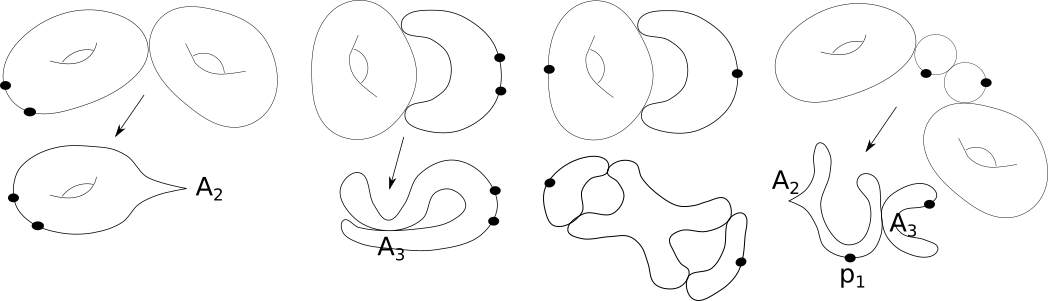
\includegraphics[width=\textwidth]{one_tail_example}
  \caption{Examples of $2$-pointed stable curves and their $1$-stable limits.}\label{fig:one_tail_example}
\end{figure}

We now have a plausible definition of $\oM_{2,2}^{(1)}$.
\begin{dfn}
 A connected, reduced, complete curve of arithmetic genus two $C$ over $\k=\bar\k$, with smooth and disjoint markings $p_1,p_2$, is \emph{$1$-stable} if:
 \begin{enumerate}[leftmargin=0.7cm]
  \item $C$ has only $A_1-,\ldots,A_4-$ and dangling $A_5-$ singularities.
  %\item Every subcurve of genus two has level $2$.
  \item There is no proper subcurve of arithmetic genus two.
  \item A subcurve of arithmetic genus one is either nodally attached and of level $3$, or it is not nodally attached and it contains $p_1$.
  %\item There is no nodally attached subcurve of genus zero.
 \end{enumerate}
\end{dfn}

The main result of the paper is that $\oM_{2,2}^{(1)}$ is a proper Deligne-Mumford stack, and the generalisation of this statement to an arbitrary number of markings and a range of stability conditions that we are going to discuss in the next subsection.

Let us note in passing that the birational map $\oM_{2,2}\dashrightarrow\oM_{2,2}^{(1)}$ is not defined everywhere. The reason boils down to the following
\begin{fact}
 There is only one isomorphism class of $2$-pointed curves whose normalisation is $(\PP^1,q_1)\sqcup(\PP^1,q_2,p_1,p_2)$ and having an $A_5$-singularity at $q_1=q_2$. On the other hand, the moduli space of $2$-pointed irreducible curves of geometric genus zero and having an $A_4$-singularity is isomorphic to $\Aaff^1$.
\end{fact}
The second statement can be motivated as follows: the pointed normalisation of such a curve is $(\PP^1,q,p_1,p_2)$, which has neither automorphisms, nor deformations. To produce an $A_4$-singularity at $q$ we may first collapse a non-zero tangent vector at $q$ (all the choices are equivalent), producing a cusp, and then collapse a line in the tangent space to the cusp, avoiding the tangent cone $\ell$ of the cusp (the moduli space is therefore $\PP^1\setminus\{\ell\}=\Aaff^1$). See Lemma \ref{lem:crimping} and the discussion thereafter.

Let $\Delta=\Delta_{1,\emptyset|0,\{1,2\}}\subseteq\oM_{2,2}$ be the divisor of rational tails, and $\mathcal W\subseteq\oM_{2,2}$ the codimension $2$ locus of Weierstrass tails. The $1$-stable limit of any point in $\Delta\setminus\mathcal W$ is the dangling $A_5$-singularity, while the $1$-stable limit of a Weierstrass tail is ill-defined (it depends on the choice of a $1$-parameter smoothing); we conjecture that the rational map (identity on the locus of smooth curves) admits a factorisation:
\bcd
& \operatorname{Bl}_{\mathcal W}(\oM_{2,2})\ar[dl]\ar[dr] & \\
\oM_{2,2}\ar[rr,dashed] & & \oM_{2,2}^{(1)}
\ecd
We plan to address this point in forthcoming work.

\subsection{Outline of results and plan of the paper} In Section \ref{sec:sing} we classify all the Gorenstein curve singularities of genus two. They come in two families: the first ($I$) one includes the ramphoid cusp, the $D_5$-singularity, and for $m\geq 3$ the union of \emph{a singular branch} (a cusp) and $m-1$ lines living in $\Aaff^m$. The second ($I\!I$) one includes the $A_5$- nd $D_6$-singularities, and for $m\geq 4$ the union of \emph{two tangent branches} (forming a tacnode) with $m-2$ lines in $\Aaff^{m-1}$. See Proposition \ref{prop:classification}.

In Section \ref{sec:crimp} we translate the condition that a complete pointed curve of genus two have no infinitesimal automorphisms into a \emph{mostly} combinatorial criterion. For every fixed number of branches $m$ and genus two singularity type $\in\{I,I\!I\}$, there are two isomorphism classes of pointed curves whose normalisation is $\bigsqcup_{i=1}^m(\PP^1,q_i,p_i)$ and having a singularity of the prescribed type at $q$; one of them has $\Aut(C,p)=\Gm$, while the other one has trivial automorphism group. This phenomenon has not emerged in lower genus. We take a detour into moduli spaces of singularities to justify the claim, and explain how to interpret the \emph{crimping spaces} geometrically in terms of the information we need to construct a genus two singularity from a (non-Gorenstein) singularity of lower genus. This is not strictly necessary in what follows, since the singularity with one-pointed branches does not satisfy the level condition we demand from our curves, yet this description is expected to be useful in analysing the indeterminacy of $\oM_{2,n}^{(m_1)}\dashrightarrow\oM_{2,n}^{(m_2)}$.

In Section \ref{sec:sstails} we study the (semi)stable limits; starting from a $1$-parameter family of semistable curves with smooth generic fiber and regular total space, we show that the shape of a subcurve of the central fiber that can be contracted into a Gorenstein singularity is strongly constrained. Singularities of type $I$ arise when the special branch (corresponding to the cusp in the contraction) is attached to a \emph{Weierstrass point} of the minimal subcurve of genus two (the \emph{core}), while singularities of type $I\!I$ occur when the special branches (corresponding to the tacnode in the contraction) are attached to \emph{conjugate points}. Furthermore, the size of the curve to be contracted only depends on one number - roughly speaking, the distance of the special branches from the core. The first statement is a consequence of the following simple observation: if $\phi\colon\widetilde{\mathcal C}\to\mathcal C$ is a contraction to a family of Gorenstein curves, $\phi^*\omega_{\mathcal C}$ is trivial on a neighbourhood of the exceptional locus of $\phi$, and it coincides with $\omega_{\widetilde{\mathcal C}}$ outside it. Now, whereas the dualising line bundle of a Gorenstein curve of genus one with no separating nodes is trivial (see \cite[Lemma 3.3]{SMY1}) and all smooth points look the same (i.e. they are not special), the simplest instance of Brill-Noether theory manifests itself in genus two, with the distinction between Weierstrass and non-Weierstrass points, and the expression $\omega_Z=\OO_Z(q+\sigma(q))$. The correct extension of these concepts to nodal curves was formulated in the '80s within the theory of admissible covers and limit linear series, and we spend some time to discuss the relevant combinatorics.

In Section \ref{sec:stability} we define the notion of \emph{$m$-stable} $n$-pointed curve of genus two, for every $1\leq m<n$. The basic idea is to trade worse singularities - of both genus one and two, bounded by $m$ in the sense of the embedding dimension - with more constraints on the combinatorics of the dual graph - the \emph{level} condition, which bounds below in terms of $m$ the number of special points (nodes and markings) that any subcurve of genus one or two has to contain. On the other hand, it is already clear from the discussion above that we need to break the $\mathfrak S_n$-symmetry, in order to write the dualising line bundle of the minimal subcurve of genus two as $\OO_Z(q_1+\sigma(q_1))$, in other words to choose which branches of a semistable model are to be dubbed special. We do so by using the first marking as a reference point, so that $q_1$ comes to denote the point of $Z$ closest to $p_1$. This shapes our algorithm to construct the $m$-stable limit of a given $1$-parameter smoothing. Unavoidably, the formulation of the stability condition is slightly involved, including a description of the interplay between $p_1$ and the singularity. Our main result is:
\begin{teo*}
 $\oM^{(m)}_{2,n}$ is a proper irreducible Deligne-Mumfod stack over $\operatorname{Spec}(\mathbb Z[\frac{1}{30}])$.
\end{teo*}


\subsection{Future directions of work} Besides regarding this as a case-study of the birational geometry of moduli spaces, we are looking forwards to applications in enumerative geometry. We set up some questions we would like to come back to.
\begin{enumerate}[leftmargin=.7cm]
 \item Resolve the indeterminacy of the rational map $\oM_{2,n}^{(m_1)}\dashrightarrow\oM_{2,n}^{(m_2)}$, and study the intersection theory of these spaces; we expect the construction to rely on a semistable compactification of the crimping spaces of the genus two singularities, as in \cite[\S 1.10]{vdW} and \cite{SMY3}. It would be interesting to put this work in the context of the Hassett-Keel program, as in \cite{SMY2}.
 
 More generally, a question outstanding to our knowledge is whether the whole program fits in the theoretical framework developed in \cite{DHLinstability}.
 
 \item We expect this work to find applications in Gromov-Witten theory. In genus one, the link between reduced Gromov-Witten invariants (see for example \cite{VZ,Zingerred,LZ}) and maps from singular curves (see \cite{VISC}) was partially uncovered in \cite{BCM}, and brought in plain view by \cite{RSPW1,RSPW2}. With F. Carocci we are investigating whether similar techniques may serve to desingularise the main component of the space of genus two maps to projective space. We expect there will be a(n iso)morphism to the modular blow-up constructed in \cite{HLN}. Maps from singular curves would provide a conceptual definition of reduced invariants for projective complete intersections and beyond, and hopefully make comparison results (standard vs. reduced) accessible. It would be interesting to relate them to Gopakumar-Vafa formulae \cite{Pandha}.
\end{enumerate}

\subsection{Acknowledgements} This project arose from discussions with Francesca Carocci, whom we thank for her availability and support. We would also like to thank Daniele Agostini, Fabio Bernasconi, Maria Beatrice Pozzetti, and Luca Tasin for helpful conversations. We thank the Max Planck Institute for Mathematics for providing financial support and a stimulating research environment.


\section{Gorenstein curve singularities of genus two}\label{sec:sing}
In this and the next sections we work over an algebraically closed field $\k$ of characteristic different from $2,3,5$. We produce an algebraic classification of the (complete) local rings of Gorenstein curve singularities of genus two.

Let $(C,q)$ be the germ of a reduced curve singularity, and let $(R,\m)$ denote $(\hat\OO_{C,q},\m_q)$, with normalisation $(\tR,\tm)\simeq\left(\k[\![t_1]\!]\oplus\ldots\oplus\k[\![t_m]\!],\langle t_1,\ldots,t_m\rangle\right)$.
Here $m$ is the number of branches of $C$ at $q$. Recall the Definition \ref{def:genus} of the genus:
\[g=\delta-m+1;\]
so, for genus two, $\delta=m+1$. Following \cite[Appendix A]{SMY1}, we consider $\tR/R$ as a $\mathbb Z$-graded module with:
\[ (\tR/R)_i:=\tm^i/(\tm^i\cap R)+\tm^{i+1};\]
furthermore, adapting Smyth's remarks in \emph{loc. cit.} to our situation:
\begin{enumerate}
\item $m+1=\delta(p)=\sum_{i\geq 0}\dim_\k(\tR/R)_i;$
\item $2=g=\sum_{i\geq 1}\dim_\k(\tR/R)_i;$
\item\label{obs:add} if $(\tR/R)_i=(\tR/R)_j=0$ then $(\tR/R)_{i+j}=0$.
\end{enumerate}
We will also make use of the following observations:
\begin{enumerate}[resume]
 \item\label{obs:igrad} $\sum_{i\geq k}(\tR/R)_i$ is a grading of $\tm^k/(\tm^k\cap R)$;
 \item\label{obs:ses} there is an exact sequence of $R/\m=\k$-modules:
 \[ 0\to A_i:=\frac{\tm^i\cap R}{\tm^{i+1}\cap R}\to \frac{\tm^i}{\tm^{i+1}}\to \left(\tR/R\right)_i\to 0\]
\end{enumerate}
\begin{lem}\label{lem:unibranch}
 There are two unibranch curve singularities of genus two; only one of them is Gorenstein, the $A_4$-singularity or \emph{ramphoid cusp}: $V(y^2-x^5)\subseteq\Aaff^2_{x,y}$.
\end{lem}
\begin{proof}
 In the unibranch case $\dim_\k(\tR/R)_1\leq 1$, hence equality holds (by observation \eqref{obs:add} above). We are left with two cases:
 \begin{itemize}[leftmargin=15pt]
  \item Either $\dim_\k(\tR/R)_2=1$ and $\dim_\k(\tR/R)_i=0$ for all $i\geq 3$: in this case $\tm^3\subseteq\m$ by observation \eqref{obs:igrad}. From \eqref{obs:ses} we see that $\tm^3=\m$, hence $R\simeq\k[\![t^3,t^4,t^5]\!],$ a spatial non-Gorenstein singularity.
  
  \item Or $\dim_\k(\tR/R)_3=1$ and $\dim_\k(\tR/R)_i=0$ for $i=2$ and for all $i\geq 4$: in this case $\tm^4\subseteq\m$ by observation \eqref{obs:igrad}. On the other hand from $\dim_\k(\tm^2\cap R/\tm^3\cap R)=1$ we deduce that there is a generator of degree $2$, and from $\dim_\k(\tm^3\cap R/\tm^4\cap R)=0$ there is none of degree $3$. We may write the generator as $x=t^2+ct^3$, and $\m=\langle x\rangle+\tm^4$. Up to a coordinate change (i.e. automorphism of $\k[\![t]\!]$), we may take $x=t^2$, and \[\m/\m^2=\langle t^2,t^5\rangle,\] so $R\simeq\k[\![x,y]\!]/(x^5-y^2)$, as anticipated.
 \end{itemize}
\end{proof}

From now on, we only look for Gorenstein singularities. With notation as above, let $I=(R:\tilde R)=\operatorname{Ann}_R(\tilde R/R)$ be the \emph{conductor ideal} of the singularity. Recall e.g. \cite[Proposition VIII.1.16]{AK}: $(C,q)$ is Gorenstein if and only if
\[\dim_\k(R/I)=\dim_\k(\tR/R)(=\delta).\]

Recall from \cite[Definition 2-1]{Stev} that a curve singularity $(C,q)$ is \emph{decomposable} if $C$ is the union of two curves $C_1$ and $C_2$ that lie in distinct smooth spaces intersecting each other transversely in $q$. Given a parametrisation $x_i=x_i(t_1,\ldots,t_m),\ i=1,\ldots,l$, this means that there is a partition $S\sqcup S^\prime=\{1,\ldots,m\}$ such that $x_i$ only depends on $t_s,s\in S$, or $s\in S^\prime$, for all $i$. Aside from the node, Gorenstein singularities are never decomposable \cite[Proposition 2.1]{AFSGm}.

\begin{prop}\label{prop:classification}
 For every fixed integer $m\geq 2$, there are exactly two Gorenstein curve singularities of genus two with $m$ branches.
\end{prop}
\begin{proof}
 We only need to find a basis for $\m/\m^2$, because a map of complete local rings that is surjective on cotangent spaces is surjective. From observation \eqref{obs:add} again, we find three possibilities for the vector $(d_1,d_2,d_3)$, $d_k=\dim_{\k}(\tR/R)_k$.
 
 \smallskip
 
 \textbf{Case} $(2,0,0)$. We see that $\tm^2\subseteq I$, so by the Gorenstein assumption we have: \[m+1=\delta=\dim_\k(R/I)\leq \dim_\k(R/\tm^2)=\dim_\k A_0+\dim_\k A_1=m-1,\] a contradiction. Note: the singularity turns out to be decomposable in this case.
 
 \smallskip
 
 \textbf{Case} $(1,1,0)$. We have $\tm^3\subseteq I$. We are going to write down the $m-1$ generators of $A_1 \pmod {\tm^3}$\footnote{To put them into the simplest possible form, we allow ourselves to perform elementary operations from linear algebra at first, while keeping ourselves from changing coordinates until the end - the benefit of this two-step process will become apparent in the next section.}. The first generator, call it $x_1$, has a non-trivial linear term in at least one of the variables, say $t_1$. By scaling $x_1$ and possibly adding a multiple of $x_1^2$, we can make it into the form:
 $x_1=t_1\oplus p_{1,2}(t_2)\oplus\ldots\oplus p_{1,m}(t_m) \pmod{\tm^3}.$ Now we can use $x_1$ and $x_1^2$ to make sure the second generator does not involve $t_1$ at all. It will still have a linear term independent of $t_1$, say non-trivial in $t_2$. By scaling and adding a multiple of $x_2^2$, we can write $x_2=0\oplus t_2\oplus\ldots\oplus p_{2,m}(t_m) \pmod{\tm^3}.$ By taking a linear combination of $x_1$ with $x_2$ and $x_2^2$, we may now reduce $x_1$ to the form $t_1\oplus0\oplus p_{1,3}(t_3)\oplus\ldots\oplus p_{1,m}(t_m)\pmod{\tm^3}$. Therefore, by Gaussian elimination with the generators and their squares, we may assume that
 \begin{align*}
  x_1= & t_1\oplus0\oplus\ldots\oplus\alpha_{1,m}t_m+\beta_{1,m}t_m^2\\
  x_2= & 0\oplus t_2\oplus\ldots\oplus\alpha_{2,m}t_m+\beta_{2,m}t_m^2\\
  &\ldots\\
  x_{m-1}= & 0\oplus\ldots\oplus t_{m-1}\oplus\alpha_{m-1,m}t_m+\beta_{m-1,m}t_m^2 \pmod{\tm^3}.
 \end{align*}
 We must have $R/I=\langle 1,x_1,\ldots,x_{m-1},y\rangle$ by the Gorenstein condition (if $x_i\in I$ for some $i$, then $t_i\in R$, and the singularity would be decomposable). Hence $x_i^2\in I$ for all but at most one $i$, say $i=1$. Then $t_i^2\in R$ for $i=2,\ldots,m-1$. If $\alpha_{i,m}\neq 0$ for some $i$ in this range, then $t_m^2\in R$ as well, so $t_1^2=x_1^2-O(t_m^2)\in R$, contradicting $\dim_\k(\tR/R)_2=1$. Therefore $\alpha_{i,m}=0$ for $i\in\{2,\ldots,m-1\}$. If $\alpha_{1,m}=0$, then we need a further generator of $\m/\m^2$, namely $z=0\oplus\ldots\oplus t_m^3$. In this case, though, both $x_1^2$ and $z$ belong to $I$, so $\dim_k(R/I)=m$, and the singularity cannot be Gorenstein. We are reduced to the following expression:
 \begin{align}\label{coordII-cs}
 \begin{split}
  x_1= & t_1\oplus0\oplus\ldots\oplus\alpha_{1,m}t_m+\beta_{1,m}t_m^2\\
  x_2= & 0\oplus t_2\oplus\ldots\oplus\beta_{2,m}t_m^2\\
  &\ldots\\
  x_{m-1}= & 0\oplus\ldots\oplus t_{m-1}\oplus \beta_{m-1,m}t_m^2 \pmod{\tm^3},
 \end{split}
 \end{align}
 with $\beta_{1,m}\in\k$ and $\alpha_{1,m},\beta_{i,m}\in\k^\times,\ i=2,\ldots,m-1$ (by indecomposability). Finally, we may change coordinates in $t_m$ and scale the other $t_i$ to obtain:
 \begin{align}\label{coordII}
 \begin{split}
  x_1= & t_1\oplus0\oplus\ldots\oplus t_m\\
  x_2= & 0\oplus t_2\oplus\ldots\oplus t_m^2\\
  &\ldots\\
  x_{m-1}= & 0\oplus\ldots\oplus t_{m-1}\oplus t_m^2\pmod{\tm^3}.
 \end{split}
 \end{align}
 We check that $R/I=\langle 1,x_1,\ldots,x_{m-1},x_1^2\rangle$ and $\tR/R$ is of type $(1,1,0)$. In case $m=2$, we need an extra generator $y=t_2^3$. Equations are given by:
 \begin{itemize}
  \item $y(y-x_1^3)$ if $m=2$ ($A_5$-singularity);
  \item $x_1x_2(x_2-x_1^2)$ if $m=3$ ($D_6$-singularity);
  \item $\langle x_3(x_1^2-x_2),x_i(x_j-x_k)\rangle_{1\leq i<j<k\leq m-1 \text{ or }1<j<k<i\leq m-1}$ if $m\geq 4$.
 \end{itemize}

 \smallskip
 
 \textbf{Case} $(1,0,1)$. We have $\tm^4\subseteq I$. By an argument similar to the above one, we write generators for $A_1$ as $x_i=\ldots\oplus t_i\oplus\ldots \oplus\alpha_{i,m}t_m+\beta_{i,m}t_m^2+\gamma_{i,m}t_m^3$, for $i=1,\ldots,m-1$.
 Then $R/I=\langle 1,x_1,\ldots,x_{m-1},y\rangle$. For all but at most one $i$, $x_i^2\in I$, but definitely $x_i^3\in I$ for all $i$. On the other hand $t_m^3\notin R$, because otherwise $t_i^3=x_i^3-\alpha_{i,m}^3t_m^3+O(t_m^4)$ would belong to $R$ as well, contradicting $\dim_\k(\tR/R)_3=1$. From this we deduce that $\alpha_{i,m}=0$ for all $i=1,\ldots,m-1$. Since $\dim_\k(\tR/R)_2=0$, there has to be another generator of $\m/\m^2$ of degree two in $t_m$, which we may write as $x_m=t_m^2+\gamma_{m,m}t_m^3$. We can use $x_m$ to remove all the $t_m^2$ pieces from $x_1,\ldots,x_{m-1}$, so we are reduced to
  \begin{align}\label{coordIII-cs}
 \begin{split}
  x_1= & t_1\oplus0\oplus\ldots\oplus \gamma_{1,m}t_m^3\\
  x_2= & 0\oplus t_2\oplus\ldots\oplus \gamma_{2,m}t_m^3\\
  &\ldots\\
  x_{m-1}= & 0\oplus\ldots\oplus t_{m-1}\oplus \gamma_{m-1,m}t_m^3\\
  x_m= & 0\oplus\ldots\oplus t_m^2+\gamma_{m,m}t_m^3 \pmod{\tm^4},
  \end{split}
 \end{align}
 with $\gamma_{m,m}\in\k$ and $\gamma_{i,m}\in\k^\times,\ i=1,\ldots,m-1$ (by indecomposability). Finally, we may change coordinates in $t_m$ and scale the other $t_i$ to obtain:
 \begin{align}\label{coordIII}
 \begin{split}
  x_1= & t_1\oplus0\oplus\ldots\oplus t_m^3\\
  x_2= & 0\oplus t_2\oplus\ldots\oplus t_m^3\\
  &\ldots\\
  x_{m-1}= & 0\oplus\ldots\oplus t_{m-1}\oplus t_m^3\\
  x_m= & 0\oplus\ldots\oplus t_m^2 \pmod{\tm^4}.
  \end{split}
 \end{align}
 We check that $R/I=\langle 1,x_1,\ldots,x_{m-1},x_m\rangle$ and $\tR/R$ is of type $(1,0,1)$. It recovers the unique Gorenstein singularity of Lemma \ref{lem:unibranch} when $m=1$. Equations are:
 \begin{itemize}
  \item $x^5-y^2$ if $m=1$ ($A_4$-singularity or \emph{ramphoid cusp}, with $x=t^2,y=t^5$);
  \item $y(y^3-x^2)$ if $m=2$ ($D_5$-singularity, with $x=x_1,y=x_2$);
  \item $\langle x_3(x_1-x_2),x_3^3-x_1x_2\rangle$ if $m=3$;
  \item $\langle x_i(x_j-x_k), x_m(x_i-x_j),x_m^3-x_1x_2\rangle_{i,j,k\in\{1,\ldots,m-1\}\text{ all different}}$ if $m\geq 4$.
 \end{itemize}
\end{proof}

%\begin{rem}
 %Not-necessarily Gorenstein singularities can be obtained by gluing various Gorenstein singularities of genus $\leq 2$ along subschemes of length $\leq 3$. Classifying all of them would not necessarily be easy.
%\end{rem}

\begin{dfn}\label{def:special_branches}
 In case $(1,0,1)$, we say the singularity is \emph{of type I}, and the branch parametrised by $t_m$ is called \emph{singular}; in case $(1,1,0)$, we say the singularity is \emph{of type II}, and the branches parametrised by $t_1$ and $t_m$ are called \emph{twin}. We shall refer to the singular or twin branches as \emph{special} or \emph{distinguished}; all other branches are \emph{axes}. \emph{Branch} remains a generic name, indicating any of the previous ones.
\end{dfn}

\begin{rem}
 Singularities of type I do appear in the miniversal family of singularities of type II, and viceversa. For low values of $m$ - which serves as the playground for our speculations -, this follows from a neat result of Grothendieck that we have learnt from \cite{C-ML} (see also \cite{Arnold,Demazure}):
 \begin{thm}\label{thm:ADE}
  Let $(C,q)$ be a curve singularity of ADE type. Singularities that appear in the miniversal deformation of $(C,q)$ are all and only those ADE, whose Dynkin diagram can be obtained as a full subgraph of the diagram of $(C,q)$.
 \end{thm}
\end{rem}


\section{Tangent sheaf, crimping space, and automorphisms}\label{sec:crimp}
In this section we analyse the tangent sheaf of a genus two singularity. For a complete Gorenstein curve of genus two with markings, we translate the absence of infinitesimal automorphisms into a (mostly) combinatorial condition. The crimping space naturally makes its appearance in the process.


\begin{lem}\label{lem:aut}
Let $(C,p)$ be a Gorenstein curve singularity of genus two, with pointed normalisation $\nu\colon(\tilde C,\{p_i\}_{i=1,\ldots,m})\to (C,p)$, and assume $\operatorname{char}(\k)\neq 2,3,5$. There is a diagram of exact sequences of sheaves
\bcd
0\ar[r]  & \nu_*\Omega_{\tilde C}^\vee(-\sum_i 3p_i)\ar[r]  &\nu_*\Omega_{\tilde C}^\vee(-\sum_i p_i)\ar[r]\ar[dr,phantom,"\Box"]  &\nu_*\bigoplus_i\Omega_{\tilde C}^\vee(-p_i)_{|2p_i}\ar[r]  & 0 \\
0\ar[r]  &\nu_*\Omega_{\tilde C}^\vee(-\sum_i 3p_i)\ar[r]\ar[u,equal]  & \Omega_C^\vee\ar[r]\ar[u] & \k^{\oplus m}\ar[r]\ar[u,hook,"\phi"] & 0
\ecd
 The right-most vertical map admits an explicit description in local coordinates.
\end{lem}
\begin{proof}
 Let $K(\tilde C)$ denote the constant sheaf of rational functions on $\tilde C$. A section of $\Omega_{\tilde C}^\vee\otimes K(\tilde C)$ is contained in $\Omega_C^\vee$ iff its image under the push-forward map
 \[\nu_*\colon\nu_*\hhom(\Omega_{\tilde C},K(\tilde C))\to \hhom(\Omega_C,K(\tilde C)) \]
 lies in the subspace $\hhom(\Omega_C,\OO_C)$. We may work locally around the singular point in the coordinates studied in the previous section.
\begin{description}
 \item[$A_4$] In the coordinates $x=t^2+ct^3,y=t^4,z=t^5$ (they are redundant, but it will not matter in what follows), the section $f(t)\frac{d}{dt}\in\nu_*\Omega_{\tilde C}^\vee\otimes K(\tilde C)$ pushes forward to
 \[\nu_*\left(f(t)\frac{d}{dt}\right)=(2t+3ct^2)f(t)\frac{d}{dx}+4t^3f(t)\frac{d}{dy}+5t^4f(t)\frac{d}{dz},\]
 from which, writing $f(t)=f_0+f_1t+f_2t^2+O(t^3)$, we see that
 \[(2t+3ct^2)f(t),4t^3f(t),5t^4f(t)\in\hat\OO_{C,p}\Leftrightarrow f_0=0,cf_1+2f_2=0.\]
 \item[$A_5$] In the coordinates $x=t_1\oplus at_2+bt_2^2,y=t_1^3$, the section $f_1(t_1)\frac{d}{dt_1}\oplus f_2(t_2)\frac{d}{dt_2}$ pushes forward to
 \[\nu_*\left(f_1(t_1)\frac{d}{dt_1}\oplus f_2(t_2)\frac{d}{dt_2}\right)=\left(f_1(t_1)\oplus (a+2bt_2) f_2(t_2)\right)\frac{d}{dx}+3t_1^2f_1(t_1)\frac{d}{dy},\]
 from which, writing $f_i(t_i)=f_{i0}+f_{i1}t_i+f_{i2}t_i^2+O(t_i^3),i=1,2$, we see that
 \[f_1(t_1)\oplus (a+2bt_2)f_2(t_2),3t_1^2f_1(t_1)\in\hat\OO_{C,p} \Leftrightarrow \begin{cases} f_{10}=f_{20}=0,\\ f_{11}=f_{21},\\ 2bf_{21}+af_{22}=a^2f_{12}.\end{cases}\]
 \item[$I\!I_{m\geq 3}$] In the coordinates of \eqref{coordII-cs},
 \begin{multline*}\nu_*\left(\sum_{i=1}^m f_i(t_i)\frac{d}{dt_i}\right)=\left(f_1(t_1)\oplus(\alpha_{1,m}+2\beta_{1,m}t_m) f_m(t_m)\right)\frac{d}{dx_1}+\\
 \sum_{i=2}^m\left(f_i(t_i)\oplus2\beta_{i,m}t_mf_m(t_m)\right)\frac{d}{dx_i},\end{multline*}
 hence we deduce that
 \[\nu_*\left(\sum_{i=1}^m f_i(t_i)\frac{d}{dt_i}\right)\in\Omega_C^\vee\otimes\hat\OO_{C,p}\Leftrightarrow \begin{cases} f_{i0}=0 & \text{for } i=1,\ldots,m,\\ 2f_{11}=f_{i1}=2f_{m1}, & \text{for } i=2,\ldots,m-1,\\ \beta_{1,m}f_{m1}+\alpha_{1,m}f_{m2}=\alpha_{1,m}^2f_{12}.\end{cases}\]
  \item[$I\!I\!I_{m\geq 2}$] In the coordinates of \eqref{coordIII-cs},
 \begin{multline*}\nu_*\left(\sum_{i=1}^m f_i(t_i)\frac{d}{dt_i}\right)=\sum_{i=1}^{m-1}\left(f_i(t_i)\oplus3\gamma_{i,m}t_m^2f_m(t_m)\right)\frac{d}{dx_i}+\\(2t_m+3\gamma_{m,m}t_m^2)f_m(t_m)\frac{d}{dx_m},\end{multline*}
 hence we deduce that
 \[\nu_*\left(\sum_{i=1}^m f_i(t_i)\frac{d}{dt_i}\right)\in\Omega_C^\vee\otimes\hat\OO_{C,p}\Leftrightarrow \begin{cases} f_{i0}=0 & \text{for } i=1,\ldots,m,\\ f_{i1}=3f_{m1}, & \text{for } i=1,\ldots,m-1,\\ 3\gamma_{m,m}f_{m1}+2f_{m2}=0.\end{cases}\]
\end{description}
\end{proof}

From this description we see that the letters $\alpha,\beta$ and $\gamma$ will play a role in determining the automorphism group of a complete curve with markings. We recall some key concepts from F. van der Wyck's thesis.

We work over $\k$. We can consider the stack $\mathcal S$ of reduced one-dimensional $\k$-algebras $R$, and the stack $\mathcal T$ of reduced 1d algebras with resolution $(R\hookrightarrow (S,J))$, where $S$ is a smooth one-dimensional $\k$-algebra, and $J$ is the radical of the conductor of $R\subseteq S$. Basically, $R$ is the (local) ring of a reduced curve with one singular point, $S$ is its normalisation, and $J$ is the ideal of the reduced fiber over the singular point of $\operatorname{Spec}(R)$. $\mathcal S$ and $\mathcal T$ are limit-preserving stacks over $\operatorname{Spec}(\k)$ \cite[Proposition 1.21]{vdW}. Furthermore, we may fix a reduced 1d algebra with resolution $\tau_0:(R_0\hookrightarrow(S_0,J_0))$, and consider the substack $\mathcal T(\tau_0)$ of reduced 1d algebras with singularity type $\tau_0$ (i.e. isomorphic to $\tau_0$ locally on both the base and the curve, see \cite[Definition 1.64]{vdW}; that various notions of ``locally'' coincide is proved in \cite[Proposition 1.50]{vdW}). There is a forgetful morphism $\mathcal T\to\mathcal S$, and the \emph{crimping space} of $\tau_0$ is defined to be the fiber over $R_0$ of the restriction of such morphism to $\mathcal T(\tau_0)$. The crimping space is a smooth $\k$-scheme \cite[Theorems 1.70 and 1.73]{vdW}; indeed, it is isomorphic to the quotient of $\Aut_{(S_0,J_0)/\k}$ by $\Aut_{(S_0,J_0)/R_0}$, the latter being the subgroup of automorphisms of the normalisation preserving the subalgebra of the singularity; moreover, the quotient can be computed after modding out the lowest power of $J$ that is contained in $R$ \cite[Theorem 1.53]{vdW}. Crimping spaces should be thought of as moduli for the normalisation map. %We shall compute the crimping space of the genus two singularities.

\begin{lem}\label{lem:crimping}
 The crimping space of a genus two singularity with $m$ branches is (a number - depending on the type - of copies of) $\Aaff^1\times(\Aaff^1\setminus\{0\})^{m-1}$.
\end{lem}
\begin{proof}
We resume notation from the previous section. We are going to fix the subalgebra $\tau_0$ given in coordinates by \eqref{coordII} and \eqref{coordIII} above respectively.

\textbf{Type II}: recall that in this case $\tm^3\subseteq R$. For a $\k$-algebra $A$, let
\[G_i(A)=\{t_i\mapsto g_{i1}t_i+g_{i2}t_i^2,t_j\mapsto t_j\ |\ g_{i1}\in A^\times,g_{i2}\in A\},\]
and notice that
\[\Aut_{(\tR,\tm)}^{\mod\tm^3}(A)=(G_1\times\ldots\times G_m)\rtimes \mathfrak{S}_m(A).\]

Consider now the action of a group element of the form $(g_1,\ldots,g_m;\id_{\mathfrak{S}_m})$ on the given generators of $R$:
\begin{align*}
 x_1\mapsto& g_{11}t_1+g_{12}t_1^2\oplus\ldots\oplus g_{m1}t_m+g_{m2}t_m^2;\\
 x_i\mapsto& \ldots\oplus g_{i1}t_i+g_{i2}t_i^2\oplus\ldots\oplus g_{m1}^2t_m^2,\quad\text{for } i=2,\ldots,m-1.
\end{align*}
The former belongs to $R$ iff $g_{11}=g_{m1}$ and $g_{12}=g_{m2}$; the latter does iff $g_{i1}=g_{m1}^2$. Thus, such elements span a subgroup isomorphic to $\Gm\times\Ga^{m-1}(A)$. On the other hand, all branches are isomorphic to one another, but there is a pair of distinguished ones (parametrised by $t_1$ and $t_m$ respectively). We conclude that
\[\Aut_{\tau_0}^{\mod\tm^3}(A)=(\Gm\times\Ga^{m-1})\rtimes(\mathfrak{S}_2\times\mathfrak{S}_{m-2})(A).\]
The quotient is then isomorphic to $\binom{m}{2}$ copies of $\Aaff^1\times(\Aaff^1\setminus\{0\})^{m-1}$.

\textbf{Type III}: in this case $\tm^4\subseteq R$. For a $\k$-algebra $A$, let
\[G_i(A)=\{t_i\mapsto g_{i1}t_i+g_{i2}t_i^2+g_{i3}t_i^3,t_j\mapsto t_j\ |\ g_{i1}\in A^*,g_{i2},g_{i3}\in A\},\]
and notice that
\[\Aut_{(\tR,\tm)}^{\mod\tm^4}(A)=(G_1\times\ldots\times G_m)\rtimes \mathfrak{S}_m(A).\]

Consider now the action of a group element of the form $(g_1,\ldots,g_m;\id_{\mathfrak{S}_m})$ on the given generators of $R$:
\begin{align*}
 x_i\mapsto& \ldots\oplus g_{i1}t_i+g_{i2}t_i^2+g_{i3}t_i^3\oplus\ldots\oplus g_{m1}^3t_m^3,\quad\text{for } i=1,\ldots,m-1;\\
 x_m\mapsto& \ldots\oplus g_{m1}^2t_m^2+2g_{m1}g_{m2}t_m^3.
\end{align*}
The former belongs to $R$ iff $g_{i1}=g_{m1}^3$; the latter does iff $g_{m2}=0$. Thus such elements span a subgroup isomorphic to $\Gm\times\Ga^{m-1}\times\Ga^m(A)$. On the other hand, there is a special (singular) branch, parametrised by $t_m$. We conclude that
\[\Aut_{\tau_0}^{\mod\tm^3}(A)=(\Gm\times\Ga^{m-1}\times\Ga^m)\rtimes(\mathfrak{S}_{m-1})(A).\]
The quotient is therefore isomorphic to $m$ copies of $\Aaff^1\times(\Aaff^1\setminus\{0\})^{m-1}$. 
\end{proof}
It is now clear that the benefit of a two-step classification where at first we do not allow ourselves to change coordinates (i.e. act by automorphisms of the normalisation) is that it makes the crimping space apparent already from the expressions \eqref{coordII-cs} and \eqref{coordIII-cs} for the generators of the singularity subalgebra.

\smallskip

There is a more geometric way to see the crimping spaces. It is well-known that a cusp can be obtained by collapsing (\emph{push-out}) a generic (i.e. non-zero) tangent vector at $p\in\PP^1$. More generally, a Gorenstein singularity of genus one and $m$ branches can be obtained by collapsing a generic (not contained in any coordinate linear subspace) tangent line at an ordinary (i.e. rational) $m$-fold point \cite[Lemma 2.2]{SMY1}. Hence, we recover the crimping space of the elliptic $m$-fold point, which is isomorphic to $(\Aaff^1\setminus\{0\})^{m-1}$, as the maximal torus inside $\PP(T_pR_m)\simeq\PP^{m-1}$, where $(R_m,p)$ is the rational $m$-fold point. Besides, this gives a natural compactification of the crimping space supporting a universal family of curves - in fact, two: either we collapse non-generic tangent vectors, obtaining non-Gorenstein singularities along the boundary (this family $\mathcal C$ has a common normalisation, that is the trivial family $\widetilde{\mathcal C}=R_m\times \PP(T_pR_m)$); or we blow-up $\widetilde{\mathcal C}$ along the boundary (\emph{sprouting}), and we replace the non-Gorenstein singularities by more elliptic $m$-fold points, this time with strictly semistable branches \cite[\S 2.2-3]{SMY2}.

Similarly, a Gorenstein singularity of genus two can be obtained by collapsing a generic tangent line to a genus one non-Gorenstein singularity. Indeed, type $\tau_0^{II}$ admits a partial normalisation by $\sigma_0^{II}$, which is the decomposable union of a tacnode in the $(t_1,t_m)$-plane together with $m-2$ axes, by adjoining the generator $t_m^2$; while type $\tau_0^{III}$ by $\sigma_0^{III}$, which is the decomposable union of a cusp (parametrised by $t_m$) together with $m-1$ axes, by adjoining $t_m^3$. These fit together nicely in the following picture: if we restrict $\mathcal C$ from the previous paragraph to the union of the coordinate lines in $\PP(T_pR_m)$, we obtain $m$ copies of $\sigma_0^{III}$ over the points, together with $\binom{m}{2}$ copies of the universal curve of type $\sigma_0^{II}$ over its crimping space - which is isomorphic to $\Aaff^1\setminus\{0\}$ -, identified with the open lines. Let $P=\PP(T_p\mathcal C_{|\cup\text{lines}})$ be the projectivised tangent space at the singular point in the fiber of this family of genus one singularities. For each of the $\binom{m}{2}$ coordinate lines, $P$ has one component $P^{II}_i$ that is a $\PP^{m-1}$-bundle over such line; besides, $P$ has $m$ components $P^{III}_j$ isomorphic to $\PP^m$ and supported over the points. The crimping space of the genus two singularities (of type II and III together) with $m$ branches can be seen to be an open subscheme of $P$: it is obtained by removing from the $\PP^{m-1}$-fibers of $P^{II}$ the $m-1$ hyperplanes generated by (a) the tangent line to the tacnode and the $m-2$ axes, and (b) the plane containing the tacnode and all but one of the $m-2$ axes; and from each component of $P^{III}$ the $m$ planes generated by (a) the tangent cone of the cusp and the $m-1$ axes, and (b) the plane containing the cusp and all but one of the $m-1$ axes.


\begin{rem}
 The crimping space is related to the moduli of arrows $\phi$ as in the diagram of Lemma \ref{lem:aut}, satisfying a number of requirements.
 
 We note that $H^0(\Omega_{\PP^1}^\vee(-p)_{|2p})$ is the tangent space to the subgroup of automorphisms of $\PP^1$ fixing one point $p$, so it is isomorphic as a Lie algebra to the only non-abelian Lie algebra of dimension two $V$. It has a basis $e_1=\begin{pmatrix} 1 & 0 \\ 0 & -1\end{pmatrix}$, $e_2=\begin{pmatrix} 0 & 0 \\ 1 & 0\end{pmatrix}$ with $[e_1,e_2]=-2e_2$. The vector $(\varphi,\psi)$ therefore corresponds to the infinitesimal automorphism: \[t\mapsto\frac{1+\epsilon\varphi t}{1-\epsilon(\varphi t+\psi)}=t+\epsilon(2\varphi t-\psi t^2).\]
 We require $\phi$ to be the embedding (i.e. a point of $\operatorname{Gr}(m,V^{\oplus m})$) of a Lie subalgebra, such that the corresponding group of infinitesimal automorphisms fixes uniquely the subalgebra of a singularity of genus two in $\k[\![t_1]\!]\oplus\ldots\oplus\k[\![t_m]\!]$.
 
 We start with some heuristics. The unibranch case goes as follows: the subalgebra of $\k[\![t]\!]$ generated by $x=t^2+ct^3$ is preserved by $(\varphi,\psi)$ iff
 \[(1+2\varphi)^2t^2-2\psi(1+2\varphi)t^3+c(1+2\varphi)^3t^3\text{ is a multiple of } t^2+ct^3,\]
 which reduces to $\varphi(1+2\varphi)c=\psi$. This furthermore determines $c$ iff $\varphi\neq 0$. Note that in this case (dimension one) the Lie subalgebra condition is automatically satisfied. We have found $(\varphi,\psi)\in\k^\times\times\k$.
 
 The case of type $I\!I_2$-algebras is more interesting. Let $x=(t_1,\alpha t_2+\beta t_2^2)$ be the generator of such an algebra. The image of $x$ under $(\varphi_1,\psi_1,\varphi_2,\psi_2)$ is:
 \[\left((1+2\varphi_1)t_1-\psi_1t_1^2,\alpha(1+2\varphi_2)t_2+(\beta(1+4\varphi_2)-\alpha\psi_2)t_2^2\right),\]
 from which we deduce:
 \begin{equation}\label{eqn:conditions}
 \varphi_1=\varphi_2\quad\text{and}\quad 2\beta\varphi_2-\alpha\psi_2=-\alpha^2\psi_1.
 \end{equation}
 Now let $\phi\colon\k^2\to V^{\oplus 2}$ be given by $\begin{pmatrix} \varphi_{11} & \psi_{11} & \varphi_{12} & \psi_{12} \\ \varphi_{21} & \psi_{21} & \varphi_{22} & \psi_{22}\end{pmatrix}$, with Pl\"ucker coordinates $w_{ij}$ for the minor of the $i$-th and $j$-th columns. The first condition in \eqref{eqn:conditions} immediately implies 
 \begin{equation}\label{eqn:vanishing_of_minors}
  w_{13}=0\quad\text{and}\quad w_{12}=-w_{23},w_{14}=w_{34}.
 \end{equation}
 The second condition in \eqref{eqn:conditions} implies
 \begin{equation}\label{eqn:nonvan_of_minors}
  \alpha w_{12}=w_{14}\quad\text{and}\quad 2\beta w_{12}=\alpha w_{24}
  \end{equation}
 so that $(\alpha,\beta)\in\k^\times\times\k$ is determined as soon as $w_{12},w_{14}\neq 0$. Notice that \eqref{eqn:vanishing_of_minors} implies in particular the Pl\"ucker equation \[w_{12}w_{34}-w_{13}w_{24}+w_{14}w_{23}.\]
 It is easy to see that the condition for $\phi$ to be a sub-Lie algebra is
 \[\operatorname{rk}\begin{pmatrix} \varphi_{11} & \psi_{11} & \varphi_{12} & \psi_{12} \\ \varphi_{21} & \psi_{21} & \varphi_{22} & \psi_{22} \\ 0 & w_{12} & 0 & w_{34} \end{pmatrix}=2,\]
 translating into 
 \begin{align*}
  w_{12}w_{13}=0 & \quad & w_{12}(w_{34}-w_{14})=0 \\ w_{13}w_{34}=0 & \quad & (w_{12}+w_{23})w_{34}=0
 \end{align*}
 which also are automatically satisfied after \eqref{eqn:vanishing_of_minors}. We see the various equations above cut inside $\PP^5_{[w_{ij}]}$ the locus \[(\Aaff^1_{{w_{14}}/{w_{12}}}\setminus\{0\})\times\Aaff^1_{{w_{24}}/{w_{12}}}.\]
 More generally, given a subalgebra $R_{\alpha,\beta}$ of $W=\bigoplus_{i=1}^m\k[\![t_i]\!]/(t_i^2)$, with generators of the form described in \eqref{coordII-cs}, the subalgebra of $V^{\oplus m}_{(\varphi_i,\psi_i)_{i=1,\ldots,m}}$ preserving $R_{\alpha,\beta}$ is isomorphic to $\k^{\oplus m}$ with equations (see Lemma \ref{lem:aut}):
 \[\begin{cases} 2\varphi_1=\varphi_i=2\varphi_m, & \text{for } i=2,\ldots,m-1,\\ 2\beta_{1,m}\varphi_m-\alpha_{1,m}\psi_m=-\alpha_{1,m}^2\psi_1;\end{cases}\]
 it is easily seen that such a subalgebra of $V^{\oplus m}$ does not determine $R_{\alpha,\beta}$, but it does determine $(\alpha_{1,m},\beta_{1,m})$. The situation of type III is analogous.
\end{rem}

We are going to use the preceding discussion in order to study the automorphism group of complete marked curves with a genus two singularity. The only case that actually requires such a discussion is when every component of the normalisation is rational and contains one extra marking, besides the preimage of the singularity: in this case it does make a difference what point of the crimping space we are looking at. The concept has been formalised again in van der Wyck's thesis, see \cite[Proposition 1.102, Theorem 1.105 and Corollary 1.106]{vdW}, where he introduces the concept of reduced pointed curve with resolution of type $T$ (encoding the amount and type of the singular points, the distribution of genus and markings among the components of the normalisation, and the adjacency data between components and singular points), and the algebraic stack $\mathcal N_T$ of such objects. In the case at hand, such stack is isomorphic to $[\Aaff^1/\Gm]$ (see also \cite[Examples 1.111-112]{vdW}), and it therefore has two points: one with $\Gm$, and the other with trivial stabiliser.

\begin{dfn}
 The \emph{atom} of type $I\!I_m$ is obtained by gluing the subalgebra of $\k[t_1]\oplus\ldots\oplus\k[t_m]$ generated by $x_1,\ldots,x_{m-1}$ (and $y$) as in \eqref{coordII} (and following lines) with $m$ copies of $(\k[s],(s))$ under the identification $s_i=t_i^{-1}$. There is a $\Gm$-action on the type II atom by $\lambda.t_i=\lambda t_i$ for $i=1,m$ and $\lambda.t_i=\lambda^2 t_i$ for $i=2,\ldots,m-1$.
 
 Similarly, the atom of type $I\!I\!I_m$ is obtained by gluing the subalgebra of $\k[t_1]\oplus\ldots\oplus\k[t_m]$ generated by $x_1,\ldots,x_m$ as in \eqref{coordIII} with $m$ copies of $(\k[s],(s))$ under the identification $s_i=t_i^{-1}$. There is a $\Gm$-action on the type III atom by $\lambda.t_i=\lambda t_i$ for $i=m$ and $\lambda.t_i=\lambda^3 t_i$ for $i=1,\ldots,m-1$.
 
 The curve with a genus two singularity and one marked point for every branch that has trivial automorphism group will be called the \emph{non-atom}.
\end{dfn}

Following the previous discussion, there is a more geometric way to realise the dicotomy between the atom and the non-atom. The non-Gorenstein genus one singularity of type $\sigma_0^{II}$ (resp. $\sigma_0^{III}$), with every branch rational and one-marked, has automorphism group $\Gm^{m-1}$ (resp. $\Gm^m$); the latter group therefore acts on the tangent space at the singular point, and it can be checked that of the lines fixed by this action only one sits inside the open subset corresponding to the crimping space, while all other lines in the open are identified under the group action - by collapsing them, they give rise to the atom and non-atom respectively.

As a third viewpoint, automorphisms can be studied by twisting the exact sequences of Lemma \ref{lem:aut} by the ideal of the markings and then taking global sections. It appears that the dicotomy arises from the map $\phi$: if the last condition imposed on infinitesimal automorphisms interweaves first and second order non-trivially (i.e. when $\beta_{1,m}$, resp. $\gamma_{m,m}$, are non-zero) then it is enough that automorphisms be trivial to second order on all branches for them to be trivial tout-court.

\smallskip

Finally, we shall turn the condition that the automorphism group be finite into a combinatorial one. For this, recall Smyth's description of Gorenstein curves of genus one with no automorphisms \cite[Proposition 2.3, Corollary 2.4]{SMY1}.

\begin{dfn}
 Let $(C,p_1,\ldots,p_n)$ be a pointed reduced curve. A connected subcurve $D\subseteq C$ is said to be \emph{nodally attached} if $D\cap\overline{C\setminus D}$ consists of nodes only.
 %Let us call a point \emph{special} if it is either a marking or a node. For a nodal and nodally attached subcurve $D$ with normalisation $\nu\colon \tilde D\to D$, pointed by $\nu^{-1}\left((\{p_1,\ldots,p_n\}\cap D)\cup (D\cap\overline{C\setminus D})\cup\{q\in D|q\text{ node of } D\}\right)$, we shall say that \emph{DM stability holds} if every rational component has at least three special points, and every elliptic component has at least one.
 We say that $C$ is \emph{residually DM} (rDM) if every nodal and nodally attached subcurve $D$ of $C$, marked by $\{p_i\in D\}\cup D\cap\overline{C\setminus D}$, is Deligne-Mumford stable.
\end{dfn}
Special points are either nodes or markings.
\begin{cor}\label{cor:explicitnoaut}
 Let $(C,p_1\ldots,p_n)$ be a pointed Gorenstein curve of arithmetic genus two. $H^0(C,\Omega_C^\vee(-\sum_{i=1}^n p_i))=0$ is equivalent to either of the following:
 \begin{enumerate}[leftmargin=.6cm]
  \item $C$ has a singularity of type $I\!I_{m\geq 2}$: either all branches contain exactly one special point and $C$ is not atomic; or at least one of its twin branches contains a special point, each of its axes contains at least one special point, and at least one branch has at least two. Furthermore $C$ is rDM.
  \item $C$ has a singularity of type $I\!I\!I_{m\geq 1}$: either all branches contain exactly one special point and $C$ is not atomic; or each of its axes contains at least one special point, and at least one branch has at least two. Furthermore $C$ is rDM.
  \item $C$ has two elliptic $m$-fold points: each of their branches contains at least one special point, and either they share a branch, or at least one branch of each singular point contains at least two special points. Furthermore $C$ is rDM.
  \item $C$ has one elliptic $m$-fold point: one of its branches is a genus one curve, or two of its branches coincide, and each of the other ones contains at least one special point; otherwise, all branches contain at least one special point, and at least one branch has at least two. Furthermore $C$ is rDM.
  \item $C$ contains only nodes and is Deligne-Mumford stable.
 \end{enumerate}
\end{cor}

\section{Dualising line bundle and semistable tails}\label{sec:sstails}

Given a family of prestable (pointed) curves of genus two over the spectrum of a discrete valuation ring $\mathcal C\to\dvr$, with smooth generic fiber $\mathcal C_{\eta}$ and regular total space, we classify the subcurves of the central fiber $\mathcal C_{0}$ that can be contracted to yield a Gorenstein singularity of genus two. In the genus one case, Smyth answered the analogous question by identifying the class of \emph{balanced} subcurves: subcurves of arithmetic genus one, such that, when breaking them into a \emph{core} (minimal subcurve of genus one, i.e. not containing any separating node) and a number of rational trees (with root corresponding to the component adjacent to the core, and leaves corresponding to the components adjacent to the portion of $\mathcal C_0$ that is not contracted), the distance between any leaf and the root for any such tree is constant. In the case at hand, the answer turns out to be slightly more complicated: first, the special branch(es) of a type I (resp. II) singularity correspond through a rational chain to a Weierstrass (resp. two conjugate) point(s) of the core, and the special branches are always the closest to the core. Second, if the core is reducible, the lengths of the rational trees may vary according to where their attaching points lie on the core, but they are determined by the length of the special chains and the configuration of the attaching points on the core.

\begin{rem}\label{rmk:Wandconj}
 While there are no special points on a smooth curve of genus zero or one, the simplest instance of Brill-Noether theory involves smooth curves of genus two. Every such $C$ is \emph{hyperelliptic}: it admits a unique (up to reparametrisation) $2:1$ cover $\phi\colon C\to\PP^1$, induced by the complete canonical linear system, i.e. $\lvert K_C\rvert$ is the unique $\mathfrak g^1_2$ on $C$; said otherwise, there is a unique element $\sigma\in\Aut(C)$, called the \emph{hyperelliptic involution}, such that $C/\langle\sigma\rangle\simeq\PP^1$. A point $x\in C$ is called \emph{Weierstrass} if it is a ramification point for $\phi$ (or, equivalently, a fixed point for $\sigma$); from the Riemann-Hurwitz formula it follows that there are six Weierstrass points on every smooth curve of genus two. Two points $x_1,x_2$ are said to be conjugate (write $x_2=\overline{x_1}$) if there exists a point $z\in\PP^1$ such that $\phi^{-1}(z)=\{x_1,x_2\}$ (or, equivalently, $\sigma(x_1)=x_2$). These notions may be extended to nodal curves by declaring $(C,x)$ to be Weierstrass if its stabilisation lies in the closure of
 \[\mathcal W=\{(C,x)|\ C\text{ smooth and } x \text{ Weierstrass}\}\subseteq\oM_{2,1},\]
 and similarly for conjugate points. We then need to study the limiting behaviour of Weierstrass points when a smooth curve degenerates to a nodal one. This is a difficult problem when it comes to higher genus curves; it has received considerable attention since the '70s, in work of Arbarello, Eisenbud-Harris, and many others. In our case it boils down to understanding admissible covers \cite{HarrisMumford} of degree two with a branch locus of degree six; said otherwise, up to the involution action, the Weierstrass locus is isomorphic to $\oM_{0,6}/\mathfrak S_5$, and the conjugate locus is isomorphic to  $\oM_{0,7}/\mathfrak S_6$. We remark that $(C,x)$ being Weierstrass is an intrinsic notion if $C$ is of compact type (or, more generally, tree-like), but it may depend on the smoothing otherwise (i.e. the fiber of $\overline{\mathcal W}\to\oM_2$ may have positive dimension); we have benefited from the exposition in \cite[Appendix 2]{Diaz}, \cite[Proposition (3.0.6)]{Cukierman}, and \cite[Theorem 5.45]{HM}.
 \begin{itemize}[leftmargin=.5cm]
  \item If $x$ belongs to a component of genus one $E$, which is attached to another component of genus one at a node $y$, then $x$ is Weierstrass iff $2x\sim 2y\in\Pic(E)$; if instead $E$ has a self-node that glues $y_1$ with $y_2$, then $x$ is Weierstrass iff $2x\sim y_1+y_2\in\Pic(E)$.
  
  If $x$ is on a rational component $R$, $x$ is Weierstrass if either $R$  is attached to a genus one curve at two distinct points, or $R$ has a self-node gluing $y_1$ and $y_2$ and is attached to a genus one tail at $y_3$, in which case we require $\phi(y_1)=\phi(y_2)$ for a double cover $\phi\colon R\to\PP^1$ ramified at $x$ and $y_3$, or $R$ has two self-nodes gluing $y_1$ with $y_2$, and $y_3$ with $y_4$, in which case we require $x$ to be a ramification point for a double cover $\phi\colon R\to\PP^1$ such that $\phi(y_1)=\phi(y_2)$ and $\phi(y_3)=\phi(y_4)$. See Figure \ref{fig:adm_W}.
  
  \begin{figure}
  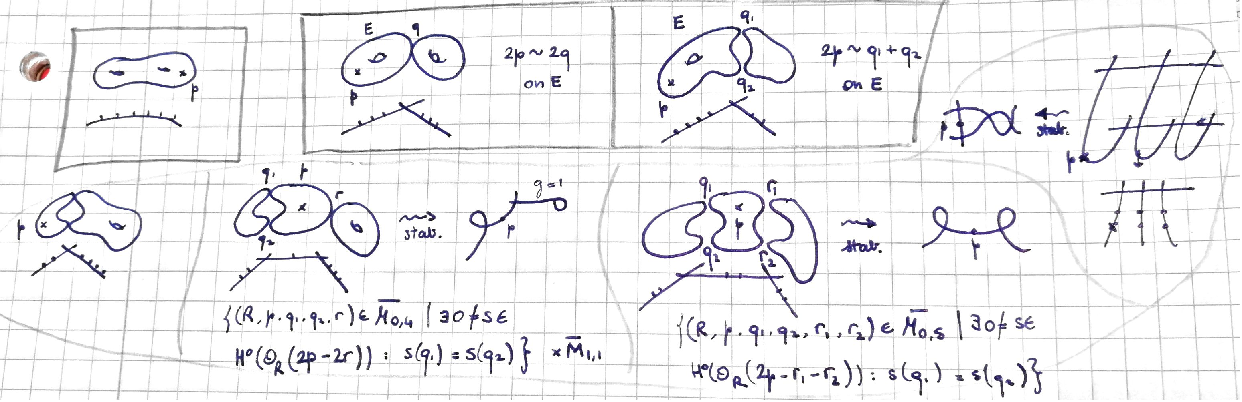
\includegraphics[width=.9\textwidth]{admissible_Weierstrass}
  \caption{Admissible covers and Weierstrass points.}\label{fig:adm_W}
  \end{figure}
 
 \item If $x_1$ and $x_2$ are conjugate, they have to map to the same component of the target of the admissible cover. The description of the previous point works by replacing every condition on $2x$ by its analogue for $x_1+x_2$.  There are a few more situations to take into account: $x_1$ and $x_2$ could belong to a rational component $R$ bubbling off from a Weierstrass point of a genus two curve; or bridging between two distinct curves of genus one; or $x_1$ and $x_2$ could lie on two distinct rational components $R_1$ and $R_2$ intersecting at one node and meeting a curve of genus one in two distinct points (\dag); or $R_1$ and $R_2$ intersecting each other in three points. See Figure \ref{fig:adm_conj}.
  \begin{figure}
 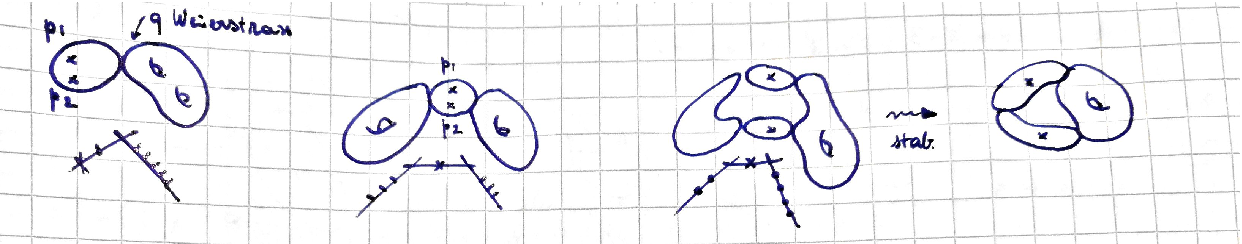
\includegraphics[width=.8\textwidth]{admissible_conjugate}  
 \caption{Admissible covers and conjugate points.}\label{fig:adm_conj}
  \end{figure}
 \end{itemize}
 We observe here that in case (\dag), the singularity of the total space of a smoothing $\mathcal C\to\dvr$ at the two distinguished nodes (separating the elliptic component from the rational chain) are both $A_k$ for the same $k$, because they map to the same node of the target in the admissible cover picture. This fact is stable under base change, and it determines a symmetry of the rational chain in the model with regular total space.
\end{rem}


\begin{prop}\label{prop:tailI}
 Let $\phi\colon\mathcal C\to\overline{\mathcal C}$ be a contraction over the spectrum of a discrete valuation ring $\dvr$, where: $\mathcal C\to \dvr$ is a family of prestable (reduced, nodal) curves of arithmetic genus two, with regular total space and smooth generic fiber $\mathcal C_{\eta}$; and $\overline{\mathcal C}\to\dvr$ is a family of Gorenstein curves of arithmetic genus two, with $\overline{\mathcal C}_{\eta}$ smooth, and $\overline{\mathcal C}_0$ containing a genus two singularity of type $I_m$ at $q$. Denote by $(Z;q_1,\ldots,q_m)$ the exceptional locus $\Exc(\phi)=\phi^{-1}(q)$, marked with $Z\cap\overline{\mathcal C_0\setminus Z}$, where $q_m$ corresponds to the special branch of $\overline{\mathcal C}_0$. Then:
 \begin{enumerate}[leftmargin=.6cm]
  \item The stabilisation of $(Z,q_m)$ is Weierstrass.
  \item Let $x_m$ be the point of the core of $Z$ closest to $q_m$, and let $k$ be the length of $R_m$, the rational chain separating $q_m$ from $x_m$. With similar notation, for every $i=1,\ldots,m-1$, $R_i$ has length 
  \begin{equation*}
  \begin{cases}
   3k+1+\dist(x_m,x_i) & \text{if } x_i\neq x_m,\\
   k+2\dist(q_m,r_i)  & \text{if } x_i=x_m,
  \end{cases} 
  \end{equation*}
 where $r_i$ is the point of $R_m$ closest to $q_i$, and $\dist(a,b)$ is the number of irreducible components between the points $a$ and $b$ (so for example it is $1$ if $a$ and $b$ lie on the same irreducible component but $a\neq b$).
 \end{enumerate}
\end{prop}

\begin{prop}\label{prop:tailII}
 Same as above with $\overline{\mathcal C}_0$ containing a genus two singularity of type $I\!I_m$, and $q_1,q_m$ corresponding to the special branches. Then:
 \begin{enumerate}[leftmargin=.6cm]
  \item The stabilisation of $(Z,q_1,q_m)$ is conjugate.
  \item $R_1$ and $R_m$ have the same length $k$, and, for $i=2,\ldots,m-1$, $R_i$ has length 
  \begin{equation*}
  \begin{cases}
   2k+\min_{\epsilon\in\{1,m\}}\dist^*(x_\epsilon,x_i) & \text{if } x_1\neq x_m, \text{ and } x_i\notin\{x_1,x_m\},\\
   k+\dist(q_1, r_i)  & \text{if } x_1\neq x_m, \text{ and } x_i=x_1 (\text{+symm. } 1\leftrightarrow m), \\
   2k+\dist(x_1,r_m)+\dist(x_1,x_i) & \text{if } x_1= x_m, \text{ and } x_i\neq x_1, \\
   k+\dist(q_1, r_i)+\delta(\dist(r_m,r_i)-1)& \text{if } x_1= x_m= x_i, \text{ and } \delta=\begin{cases} 1 & r_m\in[q_1,r_i] \\ 0 & \text{otherwise} \end{cases}
  \end{cases} 
  \end{equation*}
 where we set $\dist^*(x_\epsilon,x_i)=1$ if the core consists of a genus one curve with a rational bridge, and $x_i$ lies between $x_1$ and $x_m$ on this rational bridge, and $\dist^*(x_\epsilon,x_i)=\dist(x_\epsilon,x_i)$ otherwise.
 \end{enumerate}
\end{prop}

\begin{prop}\label{prop:contractionI}
 Let $(\mathcal C,\Sigma_1,\ldots,\Sigma_n)\to\dvr$ be a family of pointed semistable curves of arithmetic genus two such that $\mathcal C$ has regular total space and smooth generic fiber, and $(\mathcal C,\Sigma_1)\to \Delta$ is Weierstrass. Let $(Z,q_1,\ldots,q_m)$ be a genus two subcurve of $\mathcal C_0$ containing none of the $\Sigma_i(0)$, marked by $Z\cap \overline{\mathcal C_0\setminus Z}$ so that the tail containing $\Sigma_1$ is attached to $Z$ at $q_1$, and satisfying all the shape prescriptions of Proposition \ref{prop:tailI}(2). There exists a contraction $\phi\colon\mathcal C\to\overline{\mathcal C}$ over $\dvr$, with exceptional locus $Z$, such that $\overline{\mathcal C}\to\dvr$ is a family of Gorenstein curves containing a type $I_m$ singularity in the central fiber.
\end{prop}

\begin{prop}\label{prop:contractionII}
 Same as above with $(\mathcal C,\Sigma_1,\Sigma_2)\to \Delta$ conjugate, $(Z,q_1,\ldots,q_m)$ shaped as prescribed by Proposition \ref{prop:tailII}(2), and the resulting $\overline{\mathcal C}\to\dvr$ containing a type $I\!I_m$ singularity in the central fiber.
\end{prop}

\begin{proof}(of Proposition \ref{prop:tailI}) By blowing down all the rational trees on $\overline{\mathcal C}_0$, we can assume that the latter does not contain any separating node. Consider then the hyperelliptic cover $\tau\colon\overline{\mathcal C}\to\PP(\bar\pi_*\omega_{\overline{\mathcal C}/\dvr})$; restricting to the central fiber, $\tau$ contracts all axes, and gives a $2:1$ covering of $\PP^1$ by the special branch, ramified at the singularity and at another point; in fact, we can extend the image of this point to a section of $\PP(\bar\pi_*\omega_{\overline{\mathcal C}/\dvr})$ lying inside the branch locus of $\tau$. By pulling this back to $\mathcal C$ via $\tau\circ\phi$ we get a horizontal divisor $\Delta^\prime$; clearly, the stable model of $(\mathcal C,\Delta^\prime)$ is Weierstrass, and its central fiber coincides with the stabilisation of $(Z,q_1)$. This proves the first claim. (The proof of Proposition \ref{prop:tailII}(1) is entirely analogous, by noticing that the preimage of a generic hyperplane section of $\PP(\bar\pi_*\omega_{\overline{\mathcal C}/\dvr})$ will mark the two special branches of $\overline{\mathcal C}_0$.)

We now come to a proof of the more combinatorial claim (2) of the Proposition. Since $\overline{\mathcal C}\to \Delta$ is Gorenstein, and $\phi$ is assumed to be an isomorphism outside $Z$, because the dualising sheaf behaves well under restriction to open subschemes, we have an equality of line bundles:
\[ \phi^*\omega_{\overline{\mathcal C}/\dvr}=\omega_{\mathcal C/\dvr}(D),\]
for some effective (Cartier) divisor $D$ on $\mathcal C$ supported on $Z$. The next lemma will help us determine the coefficients of $D$ along the components of $Z$ containing $q_i$.

\begin{lem}\label{lem:dualising_lb}
 Let $\nu\colon C\to \bar C$ be the normalisation of a Gorenstein singularity of genus two, with $\nu^{-1}(q)=\{q_1,\ldots,q_m\}$. Then  $\nu^*\omega_{\bar C}=\omega_C(2q_1+\ldots+2q_{m-1}+4q_m)$ (type I) or $\nu^*\omega_{\bar C}=\omega_C(3q_1+2q_2+\ldots+2q_{m-1}+3q_m)$ (type II).
\end{lem}
\begin{proof}
 The dualising sheaf of a reduced curve admits an explicit description (due to Rosenlicht, see e.g. \cite[Proposition VIII.1.16]{AK}) in terms of residues:
 \[\omega_{\bar C}(U)=\{\eta\in \Omega_{C}\otimes K(\nu^{-1}(U)) | \sum_{p_i\in\nu^{-1}(p),p\in U}\operatorname{Res}_{p_i}((\nu^*f)\eta)=0,\ \forall f\in\OO_{\bar C}(U)\}.\]
 We are going to use the explicit coordinates in \eqref{coordII-cs} and \eqref{coordIII-cs}.
 In case I, we know that $\tm^4\subseteq R$, therefore we have poles of fourth order at most. It is enough to study the possible polar tails. On the other hand, $t_i^2\in R$ for all $i$ implies the part of order three is trivial. So let \[\eta=c_1\frac{\operatorname{d}t_1}{t_1^4}+b_1\frac{\operatorname{d}t_1}{t_1^2}+a_1\frac{\operatorname{d}t_1}{t_1}\oplus\ldots\oplus c_m\frac{\operatorname{d}t_m}{t_m^4}+b_m\frac{\operatorname{d}t_m}{t_m^2}+a_m\frac{\operatorname{d}t_m}{t_m}.\]
 From looking at $1\cdot\eta$ we deduce $\sum_{i=1}^m a_i=0$; from $x_i\cdot\eta$ we see $b_i+c_m=0$ for all $i$, and from $x_i^3\cdot\eta$ we have $c_i=0$ for all $i$. (The statement about third order poles can be evinced from $x_i^2\cdot\eta$ or from $z\cdot\eta$ indifferently.) Therefore $\omega_C/\nu_*\omega_{\tilde C}$ is spanned by
 \begin{align*}
  \frac{\operatorname{d}t_1}{t_1}-\frac{\operatorname{d}t_m}{t_m},\ldots,\frac{\operatorname{d}t_{m-1}}{t_{m-1}}-\frac{\operatorname{d}t_m}{t_m},\frac{\operatorname{d}t_m}{t_m^2}\\
  \bar{\eta}=\frac{\operatorname{d}t_1}{t_1^2}+\ldots+\frac{\operatorname{d}t_{m-1}}{t_{m-1}^2}-\frac{\operatorname{d}t_m}{t_m^4}.
 \end{align*}
In particular $\omega_C$ is generated by $\bar{\eta}$ as an $\OO_C$-module. 

In case II, we know that $\tm^3\subseteq R$, so we have poles of third order at most. Let \[\eta=c_1\frac{\operatorname{d}t_1}{t_1^3}+b_1\frac{\operatorname{d}t_1}{t_1^2}+a_1\frac{\operatorname{d}t_1}{t_1}\oplus\ldots\oplus c_m\frac{\operatorname{d}t_m}{t_m^3}+b_m\frac{\operatorname{d}t_m}{t_m^2}+a_m\frac{\operatorname{d}t_m}{t_m}.\]
 From looking at $1\cdot\eta$ we deduce $\sum_{i=1}^m a_i=0$; from $x_i\cdot\eta$ we see $b_1+b_m=0$ (if $i=1$), and $b_i+c_m=0$ (if $i=2,\ldots,m-1$); finally from $x_i^2\cdot\eta$ we have $c_1+c_m=0$ (if $i=1$), and $c_i=0$ (if $i=2,\ldots,m-1$). Therefore $\omega_C/\nu_*\omega_{\tilde C}$ is spanned by
 \begin{align*}
  \frac{\operatorname{d}t_1}{t_1}-\frac{\operatorname{d}t_m}{t_m},\ldots,\frac{\operatorname{d}t_{m-1}}{t_{m-1}}-\frac{\operatorname{d}t_m}{t_m},\frac{\operatorname{d}t_1}{t_1^2}-\frac{\operatorname{d}t_m}{t_m^2},\\
  \bar{\eta}=\frac{\operatorname{d}t_1}{t_1^3}+\frac{\operatorname{d}t_2}{t_2^2}+\ldots+\frac{\operatorname{d}t_{m-1}}{t_{m-1}^2}-\frac{\operatorname{d}t_m}{t_m^3}.
 \end{align*}
In particular $\omega_C$ is generated by $\bar{\eta}$ as an $\OO_C$-module.

\end{proof}

\begin{cor}\label{cor:deg_dualising}
 The dualising sheaf has multi-degree $(0,\ldots,0,2)$ (case I) and $(1,0,\ldots,0,1)$ (case II) respectively.
\end{cor}

\begin{rem}
 It follows from this computation and Corollary \ref{cor:explicitnoaut} that the finiteness condition on automorphism groups, $H^0(\bar C,\Omega_{\bar C}^\vee(-\sum_{i=1}^np_i))=0$, implies ampleness of $\omega_{\bar C}(\sum_{i=1}^np_i)$.
\end{rem}
Let us now go back to the proof of Proposition \ref{prop:tailI}. Because $\phi_{|\mathcal C_0\setminus Z}$ is the normalisation of $\overline{\mathcal C}_0$ at $q$, and, letting $T_i$ be the tail of $\mathcal C_0\setminus Z$ attached to $Z$ at $q_i$, we know that $\omega_{\mathcal C/\dvr|T_i}=\omega_{T_i}(q_i)$ by adjunction, it follows from Lemma \ref{lem:dualising_lb} that $D$ has multiplicity $3$ at the component of $Z$ containing $q_m$ in case I (resp. $2$ at the components containing $q_1$ and $q_m$ in case II), and $1$ at all other components containing a $q_i$. Set $\mathcal L=\omega_{\mathcal C/\dvr}(D)=\phi^*\omega_{\overline{\mathcal C}/\dvr}$; we shall analyse the consequences of $\mathcal L_{|Z}=\OO_Z$. We think of $Z$ as being the union of a core $K$ and a number ($\leq m$ by semistability) of rational trees.

Let $d_A$ denote the multiplicity of the divisor $D$ along the component $A$ of $Z$. First, we claim that no component can appear with $d_A=0$. Assume that this occurred along one of the rational trees. Call $S$ ($S\simeq\PP^1$) a component furthest from the core such that $d_S=0$; $R$ the one that precedes it, and $T_1,\ldots, T_h$ the ones that follow it (when sweeping the tree from the core) - so that $h\geq1$ by the previous paragraph, and $d_{T_i}\geq 1$ by inductive assumption. Then, by adjunction,
 \[\deg(\mathcal L_{|S})= -2+(h+1)+d_R+\sum d_{T_i}=0,\]
 which necessarily implies $h=1$, and $d_R=d_{T_i}=0$, contradicting the assumption. The case that $S$ belongs to the core is similar ($\omega_S$ might only be more positive).
 
Let us now consider $d_S=1$. We stick to the notation above; furthermore, there may be a number $k$ of $q_i$, $i\in\{(1,)2,\ldots,m-1\}$ in case II (resp. I), lying on $S$. Then, again by adjunction,
 \[\deg(\mathcal L_{|S})= -2+d_R+\sum d_{T_i}=0.\]
 so either $d_R=2$, $h=0$ and $k\geq 1$ arbitrary, i.e. $S$ is adjacent to $\overline{C\setminus Z}$; or $d_R=1$, $h=1$, and $d_{T_1}=1$ (with $k$ arbitrary). In the latter case, though, by repeating the same argument on $T_1$ etc., we would find an infinite chain in $Z$. 
 \begin{rem}\label{rmk:ignoring_1-trees}
  More generally, an analogous computation shows that, when balancing a component $A$ of multiplicity $d_A$, all neighbouring components of multiplicity $d_A-1$ can be safely ignored (at the same time, the number of such components is bounded only by $m$, due to the semistability of $Z$).%\footnote{define the trend along a rational chain and show it is unaltered by $\alpha-(\alpha-1)$-interactions}
 \end{rem}

 We now prove that $d_R>d_S$ holds in general for $S$ on a rational tree. The preceding paragraphs deal with the cases $d_S=0,1$; we may therefore assume $d_S>1$ (which in particular implies $0\leq k\leq 2$). We have
 \[\deg(\mathcal L_{|S})= -2+d_R-(d_S-1)(h+k+1)+\sum d_{T_i}=0.\]
 By proceeding inductively from leaves to root, we can assume that $d_S>d_{T_i},\ i=1,\ldots,h$. We may therefore rewrite the previous equality as
 \[d_R=(d_S-1)(h+k+1)-\sum d_{T_i}+2\geq(d_S-1)(k+1)+2=d_S+1+k(d_S-1)>d_S.\]
 
In fact, we can prove as on \cite[p.893]{SMY1} that $d_R=d_S+1$, unless $d_S=3$ and $q_m\in S$ (type I), or $d_S=2$ and either $q_1$ or $q_m$ (or both) are on $S$ (type II). We introduce some terminology to describe the weighted dual graph of $D$.

\begin{dfn}
 A $g$-chain is a weighted graph that is a chain and such that the weight of two adjacent vertices differ by $g$. We call $g$ the growth rate; the vertex with highest (resp. lowest) weight is called the root (resp. leaf) of the chain. An $(a,g)$-chain is a $g$-chain with leaf weight $a$. The chain $C_1$ can be attached to the chain $C_0$ by identifying the root of $C_1$ with a vertex of $C_0$ having the same weight. A $1$-tree is obtained by attaching a number of $(1,1)$-chains among themselves.
\end{dfn}

Let us now look at a component $S$ with $d_S=2$ and at least one of $q_1$ and $q_m$ attached to it. The balancing equation is
\[\deg(\mathcal L_{|S})= -2-(h+k+1)+d_R+\sum d_{T_i}=0,\]
with $k\in\{1,2\}$. The preceding discussion implies that $d_{T_i}=1$ for all $i=1,\ldots,h$, so $d_R=3+k$. If $k=2$, i.e. both $q_1$ and $q_m$ are on $S$ - in which case they are indeed equidistant from the core -, then $d_R=5$, and it can be shown inductively that the multiplicity of $D$ increases by $3$ for every step we make from $S$ towards the core. The same holds in case I, with $q_m$ attached to $S$ and $d_S=3$.

Finally, say $d_S=2$ and only $q_1\in S$. Then $d_R=4$, and the growth rate along the chain that connects $S$ to the core is $2$, unless there is a component $S^\prime$ at which two $2$-chains meet.

\begin{dfn}
 A $2$-tree is obtained by attaching a number of $(1,1)$-chains to a $(2,2)$-chain. A $3$-tree is obtained by attaching a number of $(1,1)$-chains either to a $(3,3)$-chain, or to a weighted graph itself obtained by attaching two $(2,2)$-chains to the leaf of a $3$-chain.
\end{dfn}

From the preceding discussion it is clear that the weighted dual graph of $D$ is obtained by attaching a number of $1$-trees, and either (a) one $3$-tree or (b) two $2$-trees to the dual graph of the core $K$, weighted in an appropriate fashion.

Finally, let us look at the core $K$. Consider it as a one-pointed (case (a)), resp. two-pointed (case (b)) curve of genus two, by ignoring all the attachment points of the $1$-trees (which works by Remark \ref{rmk:ignoring_1-trees}), and let $\bar K\in\oM_{2,1}$ (resp. $\oM_{2,2}$) be its stable model. The following can happen:

\begin{enumerate}[leftmargin=.6cm]

 \item $K$ is a smooth curve of genus two. In case (a), let $R$ be the component adjacent to the core along the $3$-tree, and let $x=R\cap K$; then $d_K=d_R+3$ by balancing $R$. Now balancing $K$ gives \[\omega_{\mathcal C/\dvr}(d_RR+d_KK)_{|K}=\omega_K(d_Rx-(d_R+2)x)\simeq\OO_K,\]
 which admits a solution if and only if $K$ is Weierstrass. Similarly case (b) can be balanced if and only if $K$ is conjugate.
 
 \item $K$ contains two distinct subcurves of genus one $E_1$ and $E_2$. We start by solving the balancing equation on one of them, say $E=E_1$.
 If all but one of the neighbouring components have multiplicity $d_E-1$, then the last one is forced to have multiplicity $d_E-1$ as well (by degree reasons). The case that all but two neighbouring components have multiplicity $d_E-1$ occurs when either one $2$-tree or one $3$-tree (and exactly one) is attached to $E$ at $x$; let $F$ be the other component with undetermined multiplicity, which lies between $E_1$ and $E_2$ (possibly $F=E_2$), and let $E\cap F=\{y\}$. The case of a $2$-tree forces $d_F=d_E$ by degree reason, but then we are left to solve $x\sim y$ in $\Pic(E)$, which is impossible; on the other hand, the case of a $3$-tree imposes $d_F=d_E+1$ and $2x\sim 2y$ in $\Pic(E)$, i.e. $K$ is Weierstrass. By the same token, the two $2$-trees have two hit the same genus one curve, say $E_1$, in nodes $x_1,x_2$ such that $x_1+x_2\sim 2y$ and $d_F=d_E+1$.
 
 Assume now that there is a chain of rational curves $S_i$ lying between $E_1$ and $E_2$ in $K$, and one of the special trees connects to one of the $S_i$; in case (b), then, both $2$-trees must connect to (possibly different) $S_i$, by the previous paragraph. Furthermore, the growth rate along the rational chains at $E_1$ and $E_2$ has to be $1$. This in turn implies that, in case (b), the growth rate along the chain separating the two $2$-trees is $0$. In particular, the two $2$-trees are attached to components with the same multiplicity for $D$, so $q_1$ and $q_m$ are equidistant from the core. See Figure \ref{fig:E1E2} for some examples.
 
 \begin{figure}
 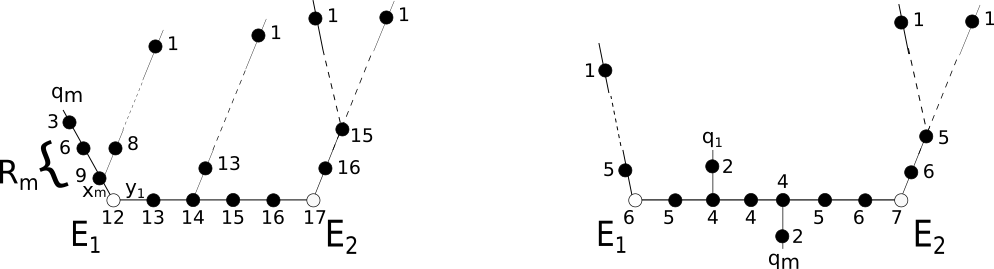
\includegraphics[width=.8\textwidth]{E1E2example} 
 \caption{Examples of $Z$ with two genus one components (the white dots). The numbers indicate the multiplicity of $D$. On the left, one $3$-tree attached to $E_1$; on the right, two $2$-trees attached to the same bead of the rational chain separating $E_1$ from $E_2$.}\label{fig:E1E2}
  \end{figure}
  
 \item $\bar K\in\Delta_{irr}$, i.e. $K$ contains an irreducible subcurve of arithmetic genus one $E$, with two points $y_1$ and $y_2$ on $E$ that are joined in $K$ by a (possibly empty) rational chain. We see as above that either a $3$-tree is attached to a point $x\in E$ satisfying $2x\sim y_1+y_2$ in $\Pic(E)$, or two $2$-trees are attached to $x_1,x_2\in E$ satisfying $x_1+x_2\sim y_1+y_2$ in $\Pic(E)$, or the rational chain is not empty and all the distinguished trees are attached to it. In this case, solve the balancing equation on $E$: let $d=d_E$, $d_1$ and $d_2$ be the multiplicities of the rational components attached to $y_1$ and $y_2$ respectively; then either $d_1=d_2=d-1$, or $d_1=d-1+k$, $d_2=d-1-k$ and $r_1-r_2$ is $k$-torsion in $\Pic(E)$. But, by chasing the balancing equation along the rational necklace, we find that, if $k\geq 1$, then the growth rate increases when passing through a distinguished bead, so that ultimately $d-1-k=d_2>d_1d-1+k$, which is absurd. So the only possibility is to have a rational chain symmetric with respect to the distinguished beads, namely: in case (a) the two pieces of the rational chain standing between the special bead and $E$ have the same length, and in case (b) the distance shortest path between a special bead and $E$ is the same for the two special beads. See Figure \ref{fig:ER}.
 
  \begin{figure}
 \includegraphics[width=.8\textwidth]{ERexample}
 \caption{$K$ is a genus one curve $E$ with a rational bridge $R$. Left column, one $3$-tree; right, two $2$-trees. Above: the special trees cleave to $E$; below: they cleave to $R$ - note that $R$ is necessarily symmetric in this case.}\label{fig:ER}
  \end{figure}
 
 \item Finally, we consider the case that $K$ has geometric genus $0$. It is easy to see that, if a special tree cleaves to a stable component, the only chance that the balancing condition may be satisfied is that there are two $2$-trees and they cleave to different stable components; the semistable chains have arbitrary length and $D$ has the same multiplicity along every component of the core; see the upper left corner of Figure \ref{fig:Krat}. There remain three possibilities for the dual graph, according to how the distinguished components (denoted by $R$) and the other stable components (denoted by $A$ and $B$) distribute themselves.
  \begin{figure}
 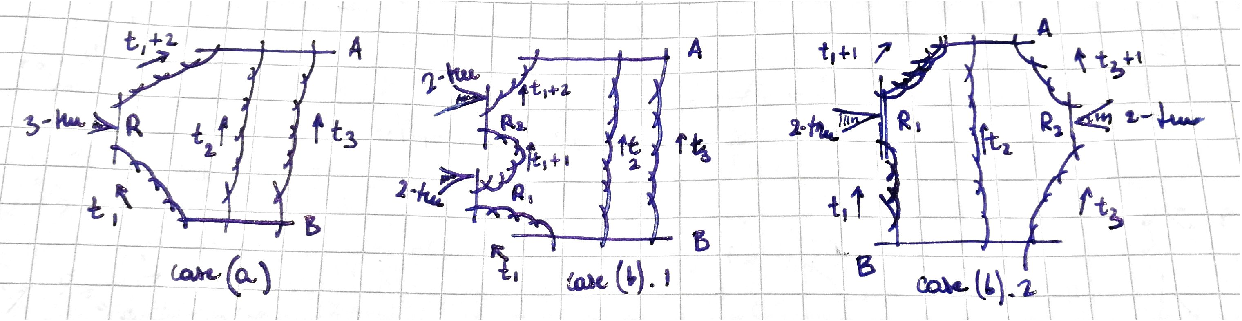
\includegraphics[width=.8\textwidth]{rational_pretzel} 
 \caption{When $K$ consists of rational curves.}\label{fig:Krat}
  \end{figure}
 Denoting by $t$ the growth rate along various rational chains, we find that in case (a) and (b).1 balancing along $A$ or $B$ is equivalent to $\sum_it_i=1$. Assume $t_1\geq0$; then $d_A>d_B$, therefore $t_2,t_3>0$, which contradicts $\sum_it_i=1$. Similarly, if $t_1\leq -2$, then $d_A<d_B$, therefore $t_2,t_3<0$, which makes $\sum_it_i=1$ again impossible. We find only one solution with $t_1=-1$ and $t_2=t_3=0$ - notice that it is a degeneration of the case considered in the previous point.
 On the other hand, in case (b).2, we find $\sum_it_i=1$ when balancing $B$, and $\sum_it_i=-1$ when balancing $A$, which is a contradiction.
\end{enumerate}
This concludes the proof of Propositions \ref{prop:tailI}(2) and \ref{prop:tailII}(2).
\end{proof}
\begin{rem}\label{rmk:extra_conjugate}
There is a stable $2$-pointed curve that arises as a solution of the balancing equation, yet is not conjugate, namely:
  \begin{center}
 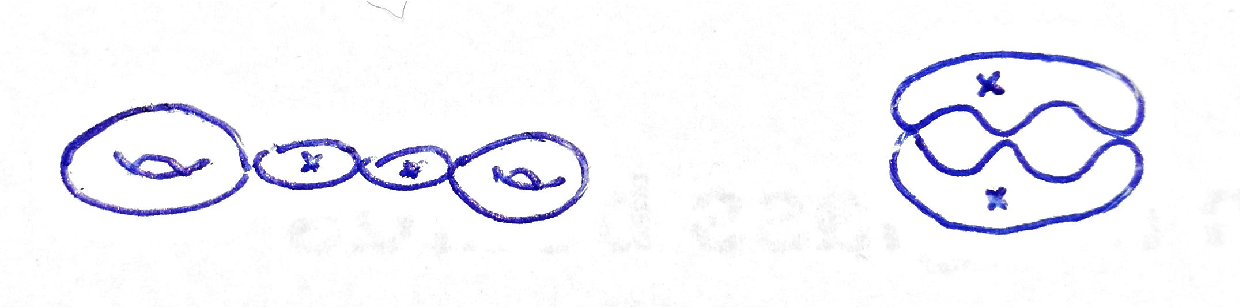
\includegraphics[width=.6\textwidth]{extra_conjugate}  
  \end{center}
In this case, the line bundle $\omega_{\mathcal C/\dvr}(D)$ trivial along $Z$ might not be semiample.
\end{rem}


\begin{proof}(of Proposition \ref{prop:contractionI})
 By blowing down some rational tails outside $Z$, we can assume that $\mathcal C_0\setminus Z=\sqcup_{i=1}^m T_i$ with each $T_i\simeq\PP^1$. The image of $\Sigma_i(0)$ and $\Sigma_j(0)$ may now coincide for $i\neq j$. The total space of the curve can still be assumed to be smooth. By abuse of notation, we denote the resulting family of pointed curves by $(\mathcal C,\Sigma_1,\ldots,\Sigma_n)$. By assumption on the shape of $Z$, we can find an effective Cartier $D$ supported on $Z$ such that $\mathcal L=\omega_{\mathcal C/\dvr}(D+\Sigma)$ be trivial on $Z$ and relatively ample elsewhere (both on $T_i$ and on the generic fiber). Consider a second line bundle $\mathcal L^\prime=\OO(2\Sigma_1+\Sigma)$. Since we assumed $\Sigma_1$ to be Weierstrass, $\mathcal L_\eta\simeq\mathcal L^\prime_\eta$. On the other hand it is easy to see that the multi-degrees of $\mathcal L_0$ and $\mathcal L^\prime_0$ coincide; it follows from the separatedness of $\Pic^0_{\mathcal C/\dvr}\to\dvr$ (see \cite[p. 136]{Deligne} or \cite[\S 9.4]{BLR}) that $\mathcal L$ and $\mathcal L^\prime$ are isomorphic line bundles, so that in particular $\mathcal L$ is trivial on a neighbourhood of $Z$. Observe now that 
 \[R^1\pi_*\mathcal L(-D)= R^1\pi_*\omega_{\mathcal C/\dvr}(\Sigma)=0\]
 by semistability, hence $\pi_*\mathcal L\twoheadrightarrow \pi_*(\mathcal L_{|D})=\pi_*\OO_D$ which contains the constants, showing that $\mathcal L$ is semiample along $Z$ (that it is along the $T_i$ is easier). We therefore have a contraction
 \[\mathcal C\xrightarrow{\phi}\overline{\mathcal C}=\underline{\operatorname{Proj}}_\dvr\left(\bigoplus_{n\geq 0}\pi_*\mathcal L^{\otimes n}\right)\to\dvr\]
 associated to $\mathcal L$. The proof that $\overline{\mathcal C}\to \dvr$ is a flat family of Gorenstein curves goes along the lines of \cite[Lemma 2.13]{SMY1} or \cite[Proposition 3.7.3.1]{RSPW1}. It is the clear from the classification that it contains a type $I_m$-singularity in the central fiber. The proof of Proposition \ref{prop:contractionII} is entirely analogous.
\end{proof}


\begin{caveat}
 It seems not to be true in general that, if we have a family of semistable curves $\pi\colon\mathcal C\to\dvr$ over a discrete valuation ring, and a line bundle $\mathcal L$ on $\mathcal C$ that is trivial on a higher genus subcurve $Z$ of $\mathcal C_0$, and $\pi$-ample elsewhere, then $\mathcal L$ is $\pi$-semiample, i.e. relatively generated by global sections. It will rather depend on the family, and, in particular, the assumption that the total space of $\mathcal C$ is regular along $Z$ seems to be essential. This seems not to be an issue in positive characteristic, thanks to a result of S. Keel \cite{Keel-bpf}, so assume $\operatorname{char}(\k)=0$; we give a counterexample using the theory of limit linear series: we produce a linear series that can be smoothed while having basepoints along a Weierstrass tail.\footnote{It has been pointed out to us by F. Carocci that a similar but easier computation can be carried out for a genus one tail as well. This shows that the regularity assumption of \cite[Lemma 2.13]{SMY1} is necessary.} For any such smoothing, the corresponding line bundle $\mathcal L$ is not globally generated along $Z$ - though we do not know how the powers of $\mathcal L$ behave.
 
 Let $X_0$ be the nodal curve obtained by attaching $R\simeq\PP^1$ to a Weierstrass point $q$ of a smooth genus two curve $Z$. Choose $d\gg 0$ ($d\geq5$ is enough), and let us study the moduli space of complete linear systems of degree $d$ on (smoothings of) $X_0$; with $r=d-2$, the Brill-Noether number is $\rho=2$ (the dimension of the Jacobian). On the other hand, assume that the $R$-aspect of the lls has $\mathcal L_{Y|Z}\simeq\OO_Z$; then the $Z$-aspect has $\mathcal L_{Z|Z}\simeq\OO_Z(dq)$, whose vanishing sequence is $\alpha_Z(q)=\{0,1,\ldots,d-4,d-2,d\}$, from which we deduce for the complementary aspect $\alpha_R(q)\geq\{0,2,4,5,\ldots,d\}$. We want to show that all such aspects are smoothable, by appealing to the Regeneration Theorem \cite[Theorem 5.41]{HM}. Notice that in the case at hand we have a choice of a two-dimensional subspace of $\langle 1,t,t^2,t^3\rangle_\k\subseteq H^0(\PP^1,\OO_{\PP^1}(d))$ meeting the subspace $\langle t^2,t^3\rangle_\k$ non-trivially, i.e. the locus in $\operatorname{Gr}(1,\PP^3)$ of lines meeting a fixed line $\ell$, which is a Schubert cycle of dimension $3$. We therefore need to put $X_0$ in a family over a base $B$ of dimension $1$ at least.  We shall do so by considering the family $X$ obtained by attaching $R$ to a moving point of $Z$, so that $X_0$ is the fiber of $X$ over $q\in Z$.
 
 Let us start by examining the other possibilities for $\mathcal G^{d-2}_d(X_0)$: the $R$-aspect can in fact restrict to any line bundle of degree $0$ on $Z$, which we are going to write as $\OO_Z(p_1+p_2-2q)$ for two moving points $p_1,p_2$ on $Z$ (think of them as coordinates on $\Pic(Z)$). Then $\mathcal L_Z=\OO_Z((d-2)q+p_1+p_2)$.
 
 \hspace{-.7cm} \begin{tabular}{lc|c|c|cr}
  $\subseteq\Pic(Z)$ & dim & $\alpha_{Z;d-3,d-2}$ & $\alpha_{R;0,1}$ & $\subseteq \PP H^0(R,\OO_R(d))$ & dim \\ \hline
  $p_1+p_2\sim 2q$ & $0$ & $\{d-2,d\}$ & $\geq\{0,2\}$ & $\{\ell^\prime\in\operatorname{Gr}(1,\PP^3)|\ell^\prime\cap\ell\neq\empty
  \}$ & $3$\\
  $2q\nsim p_1+p_2\geq q$ & $1$ & $\{d-3,d-1\}$ & $\geq\{1,3\}$ & $\PP^1$ & $1$\\
  $p_1+p_2\ngeq q$ & $2$ & $\{d-3,d-2\}$ & $\{2,3\}$ & pt & $0$\\
 \end{tabular}

 If we now let $q$ vary in $B\simeq Z$, we may generically assume that it is not Weierstrass. We then find the following:
 
 \hspace{-.7cm} \begin{tabular}{lc|c|c|cr}
  $\subseteq\Pic(X)$ & dim & $\alpha_{Z;d-3,d-2}$ & $\alpha_{R;0,1}$ & $\subseteq\PP H^0(R,\OO_R(d))$ & dim \\ \hline
  $p_1+p_2\sim \omega_Z$ & $0+1$ & $\{d-2,d-1\}$ & $\geq\{1,2\}$ & $(\PP^{2})^*$ & $2$\\
  $p_1+p_2\sim 2q$ & $0+1$ & $\{d-3,d\}$ & $\geq\{0,3\}$ & $\PP^2$ & $2$\\
  $\omega_Z,2q\nsim p_1+p_2\geq q$ & $1+1$ & $\{d-3,d-1\}$ & $\geq\{1,3\}$ & $\PP^1$ & $1$\\
  $p_1+p_2\ngeq q$ & $2+1$ & $\{d-3,d-2\}$ & $\{2,3\}$ & pt & $0$\\
 \end{tabular}
 
 We conclude that $\mathcal G^{d-2}_d(X/B)$ has pure dimension $3$, and we may therefore apply the Regeneration Theorem to deduce that all lls with $\mathcal L_{R|Z}\simeq\OO_Z$ - in particular those with base-locus $Z$ - are smoothable.
\end{caveat}

\begin{comment}
section{Dualising line bundle and semistable tails - old}
This is the most technical and combinatorially delicate section of the paper. We classify the nodal subcurves that can be contracted in a one-parameter smoothing in order to obtain a Gorenstein singularity of genus two. The upshot is that the distinguished (i.e. twin or singular) branches are attached to special (i.e. conjugate or Weierstrass) points of the core (minimal subcurve of genus two). That said, the shape of the contracted curve depends on one parameter only, namely the distance of the distinguished branch(es) from the core - parallel to Smyth's \emph{balanced} condition \cite[Definition 2.11]{SMY1} in genus one, and its generalisation by the strict interior of a circle around the circuit in \cite{RSPW1}. This is going to play a key role in the proof that our moduli spaces are proper.

\begin{lem}\label{lem:contraction}
 Let $\pi\colon\mathcal C\to\dvr$ be a family of nodal curves over a DVR, and let $\mathcal L$ be a line bundle on $\mathcal C$ that is trivial \emph{on a neighbourhood} of a connected subcurve $Z$ of genus two in the central fiber $C=\mathcal C_0$, and $\pi$-ample everywhere else. Assume that $\mathcal C$ is regular along $Z$. Then $\mathcal L$ is $\pi$-semiample. Setting \[\phi\colon\mathcal C\to \mathcal C^\prime=\Proj_\dvr\left(\bigoplus_{n\geq0}\pi_*\mathcal L^{\otimes n}\right),\] $\mathcal C^\prime$ is a flat family of reduced curves, and $C^\prime$ has a genus two singularity at $q=\phi(Z)$ with $m=\lvert Z\cap\overline{C\setminus Z}\rvert$ branches, whose normalisation is $\phi_{\lvert\overline{C\setminus Z}}$. Moreover, $q$ is a Gorenstein singularity if and only if $\mathcal L$ can be written in the form $\omega_{\mathcal C/\dvr}(D+\Sigma)$, where $D$ is supported on $Z$ and $\Sigma$ is supported away from $Z$.
\end{lem}
\begin{proof}
 This is a straightforward extension of Smyth's contraction lemma \cite[Lemma 2.13]{SMY1}. Up to substituting $\mathcal L$ by a sufficiently high power of itself, we claim that there exists a divisor $D^\prime$ on $\mathcal C$, supported on $Z$, such that $R^1\pi_*\mathcal L(-D^\prime)=0$. Indeed, if $\lev(Z)=\lvert Z\cap\overline{C\setminus Z}\rvert\geq 3$, it is enough to take $D^\prime=Z$, by cohomology and base-change, and Serre duality. On the other hand, if $Z$ is either a conjugate bridge or a Weierstrass tail (we leave the discussion of the other possible situations, since they will not occur in what follows), we have to go through a case-by-case analysis:
 \begin{itemize}[leftmargin=.3cm]
  \item if $Z$ is irreducible, it is enough to take $D^\prime=3Z$ (in fact, $2Z$ when $Z$ is a bridge);
  \item if $Z=E_1\sqcup_q E_2$ is the union of two curves of genus one, attached to the rest of $C$ along $E_1$, then $D^\prime=2E_1+3E_2$ suffices;
  \item if $Z=E\sqcup_{\{q_1,q_2\}} R$ is the union of a genus one curve with a rational bridge, attached to the rest of $C$ along $E$, take $D^\prime=2E+3R$; while take $D^\prime=3E+2R$ if the same $Z$ is attached to the rest of $C$ along $R$;
  \item if $Z$ is formed of three rational components such that $R_1\cap R_2$ is two nodes, $R_1\cap R_0$ and $R_2\cap R_0$ are each one node, and the rest of $C$ is attached to $Z$ along $R_0$, then it is enough to choose $D^\prime=3R_0+4R_1+4R_2$.
 \end{itemize}
 Similar solutions can be found if $Z$ contains rational trees, or if a rational curve is replaced by a chain in the above. The vanishing of $R^1\pi_*\mathcal L(-D^\prime)$ implies that $\pi_*\mathcal L$ surjects onto $\pi_*\mathcal L_{|D^\prime}=\pi_*\OO_{D^\prime}$, by the assumption that $\mathcal L$ is trivial on a neighbourhood of $Z$. On the other hand, $Z=(D^\prime)_{\mathrm{red}}$ implies that $H^0(D^\prime,\OO_{D^\prime})\twoheadrightarrow H^0(Z,\OO_Z)=\k$, hence $\mathcal L$ is globally generated along $Z$. The remaining assertions have been proved by Smyth (\emph{loc. cit.}; see also \cite[Proposition 3.7.3.1]{RSPW1}). 
\end{proof}

\begin{rem}
 The assumption that the total space of $\mathcal C$ is regular along $Z$ seems to be necessary for $\mathcal L$ to be generated by global sections along $Z$. Assume $\operatorname{char}(\k)=0$\footnote{This is in fact not an issue in positive characteristic, thanks to a result of S. Keel \cite{Keel-bpf}.}; using the theory of limit linear series, we show that for certain line bundles $\mathcal L$ - trivial on $Z$ and ample elsewhere - on certain one-parameter smoothings of a genus two tail $Z$, the associated complete linear system has base-points along $Z$. We do not know how the powers of $\mathcal L$ behave, though.
 
 Let $X_0$ be the nodal curve obtained by attaching $R\simeq\PP^1$ to a Weierstrass point $q$ of a smooth genus two curve $Z$. Choose $d\gg 0$ ($d\geq5$ is enough), and let us study the moduli space of complete linear systems of degree $d$ on (smoothings of) $X_0$; with $r=d-2$, the Brill-Noether number is $\rho=2$ (the dimension of the Jacobian). On the other hand, assume that the $R$-aspect of the lls has $\mathcal L_{Y|Z}\simeq\OO_Z$; then the $Z$-aspect has $\mathcal L_{Z|Z}\simeq\OO_Z(dq)$, whose vanishing sequence is $\alpha_Z(q)=\{0,1,\ldots,d-4,d-2,d\}$, from which we deduce for the complementary aspect $\alpha_R(q)\geq\{0,2,4,5,\ldots,d\}$. We want to show that all such aspects are smoothable, by appealing to the Regeneration Theorem \cite[Theorem 5.41]{HM}. Notice that in the case at hand we have a choice of a two-dimensional subspace of $\langle 1,t,t^2,t^3\rangle_\k\subseteq H^0(\PP^1,\OO_{\PP^1}(d))$ meeting the subspace $\langle t^2,t^3\rangle_\k$ non-trivially, i.e. the locus in $\operatorname{Gr}(1,\PP^3)$ of lines meeting a fixed line $\ell$, which is a Schubert cycle of dimension $3$. We therefore need to put $X_0$ in a family over a base $B$ of dimension $1$ at least.  We shall do so by considering the family $X$ obtained by attaching $R$ to a moving point of $Z$, so that $X_0$ is the fiber of $X$ over $q\in Z$.
 
 Let us start by examining the other possibilities for $\mathcal G^{d-2}_d(X_0)$: the $R$-aspect can in fact restrict to any line bundle of degree $0$ on $Z$, which we are going to write as $\OO_Z(p_1+p_2-2q)$ for two moving points $p_1,p_2$ on $Z$ (think of them as coordinates on $\Pic(Z)$). Then $\mathcal L_Z=\OO_Z((d-2)q+p_1+p_2)$.
 
 \hspace{-.7cm} \begin{tabular}{lc|c|c|cr}
  $\subseteq\Pic(Z)$ & dim & $\alpha_{Z;d-3,d-2}$ & $\alpha_{R;0,1}$ & $\subseteq \PP H^0(R,\OO_R(d))$ & dim \\ \hline
  $p_1+p_2\sim 2q$ & $0$ & $\{d-2,d\}$ & $\geq\{0,2\}$ & $\{\ell^\prime\in\operatorname{Gr}(1,\PP^3)|\ell^\prime\cap\ell\neq\empty
  \}$ & $3$\\
  $2q\nsim p_1+p_2\geq q$ & $1$ & $\{d-3,d-1\}$ & $\geq\{1,3\}$ & $\PP^1$ & $1$\\
  $p_1+p_2\ngeq q$ & $2$ & $\{d-3,d-2\}$ & $\{2,3\}$ & pt & $0$\\
 \end{tabular}

 If we now let $q$ vary in $B\simeq Z$, we may generically assume that it is not Weierstrass. We then find the following:
 
 \hspace{-.7cm} \begin{tabular}{lc|c|c|cr}
  $\subseteq\Pic(X)$ & dim & $\alpha_{Z;d-3,d-2}$ & $\alpha_{R;0,1}$ & $\subseteq\PP H^0(R,\OO_R(d))$ & dim \\ \hline
  $p_1+p_2\sim \omega_Z$ & $0+1$ & $\{d-2,d-1\}$ & $\geq\{1,2\}$ & $(\PP^{2})^*$ & $2$\\
  $p_1+p_2\sim 2q$ & $0+1$ & $\{d-3,d\}$ & $\geq\{0,3\}$ & $\PP^2$ & $2$\\
  $\omega_Z,2q\nsim p_1+p_2\geq q$ & $1+1$ & $\{d-3,d-1\}$ & $\geq\{1,3\}$ & $\PP^1$ & $1$\\
  $p_1+p_2\ngeq q$ & $2+1$ & $\{d-3,d-2\}$ & $\{2,3\}$ & pt & $0$\\
 \end{tabular}
 
 We conclude that $\mathcal G^{d-2}_d(X/B)$ has pure dimension $3$, and we may therefore apply the Regeneration Theorem to deduce that all lls with $\mathcal L_{R|Z}\simeq\OO_Z$ - in particular those with base-locus $Z$ - are smoothable.\footnote{It has been pointed out to us by F. Carocci that a similar but easier computation can be carried out for a genus one tail as well.}
\end{rem}

The following lemma is useful in determining the multiplicity of $D$ (as in Lemma \ref{lem:contraction}) along components of $Z$ adjacent to $\overline{C\setminus Z}$.

\begin{comment}
\begin{rem}\label{rmk:contraction}
 We are going to produce line bundles on smoothings of nodal curves that are trivial on a genus two subcurve $Z$ of the central fiber, and have positive degree on all other components of the fibers; so they are suitable to produce a contraction of $Z$, as soon as they are globally generated over the base. We postpone the discussion of this issue until when we have described such line bundles explicitly. For now we content ourselves to observe that a na\"ive extension of Smyth's contraction lemma \cite[Lemma 2.13]{SMY1} does not seem to hold.
\end{rem}

\begin{lem}\label{lem:general_contraction}
 Let $\pi\colon\mathcal C\to\dvr$ be a family of nodal curves over a DVR, and let $\mathcal L$ be a line bundle on $\mathcal C$ that is trivial on a connected subcurve $Z$ of genus two in $C=\mathcal C_0$, and $\pi$-ample otherwise. Assume that $\mathcal C$ is regular along $Z$ and that \[\lev(Z)=\lvert Z\cap\overline{C\setminus Z}\rvert\geq 3.\] Then $\mathcal L$ is $\pi$-semiample. Setting $\phi\colon\mathcal C\to \mathcal C^\prime=\Proj_\dvr\left(\bigoplus_{n\geq0}\pi_*\mathcal L^{\otimes n}\right)$, $\mathcal C^\prime$ is a flat family of reduced curves, and $C^\prime$ has a genus two singularity at $q=\phi(Z)$ with $m=\lvert Z\cap\overline{C\setminus Z}\rvert$ branches, whose normalisation is $\phi_{\lvert\overline{C\setminus Z}}$.
\end{lem}
\begin{proof}
 Smyth's proof (\emph{loc.cit.}) works unchanged. We review it quickly. Up to replacing $\mathcal L$ with a sufficiently high power of itself, $R^1\pi_*\mathcal L(-Z)=0$, so $\pi_*\mathcal L$ surjects onto $\pi_*\OO_Z$, thus having a section not vanishing along $Z$. The vanishing of $R^1\pi_*\mathcal L(-Z)$ follows from cohomology and base-change, since the restriction of $\mathcal L(-Z)$ to $Z$ has degree equal to $\lev(Z)\geq 3$ by assumption, so $h^1=0$.
\end{proof}

\begin{lem}\label{lem:Gorenstein_contraction}
 Let $\phi\colon\mathcal C\to \mathcal C^\prime$ be a $\dvr$-contraction induced by a line bundle $\mathcal L$ on $\mathcal C$, as above. Then $\mathcal C^\prime$ is a family of Gorenstein curves if and only if $\mathcal L$ can be written in the form $\mathcal L=\omega_{\mathcal C/\dvr}(D+\Sigma)$ for some effective divisors $D$ supported on $\Exc(\phi)$, and $\Sigma$ supported away from $\Exc(\phi)$.
\end{lem}
\begin{proof}
 $\omega_{\mathcal C^\prime/\dvr}$ and $\OO_{\mathcal C^\prime}(1)(-\phi(\Sigma))$ are $S_2$-sheaves isomorphic outside a codimension two locus, therefore they coincide and the former is a line bundle. See the proof of \cite[Lemma 2.13]{SMY1} and \cite[Proposition 3.7.3.1]{RSPW1}.
 %Follows from some place in Koll\'ar-Mori.
\end{proof}

\begin{customrmk}{4.1(continued)}
 %This is a follow-up to Remark \ref{rmk:contraction}.
 Assume $\operatorname{char}(\k)=0$\footnote{This is in fact not an issue in positive characteristic, thanks to a result of S. Keel \cite{Keel-bpf}.}; using the theory of limit linear series, we show that for certain line bundles $\mathcal L$ - trivial on $Z$ and ample elsewhere - on certain one-parameter smoothings of a genus two tail $Z$, the associated complete linear system has base-points along $Z$. We do not know how the powers of $\mathcal L$ behave, though.
 
 Let $X_0$ be the nodal curve obtained by attaching $R\simeq\PP^1$ to a Weierstrass point $q$ of a smooth genus two curve $Z$. Choose $d\gg 0$ ($d\geq5$ is enough), and let us study the moduli space of complete linear systems of degree $d$ on (smoothings of) $X_0$; with $r=d-2$, the Brill-Noether number is $\rho=2$ (the dimension of the Jacobian). On the other hand, assume that the $R$-aspect of the lls has $\mathcal L_{Y|Z}\simeq\OO_Z$; then the $Z$-aspect has $\mathcal L_{Z|Z}\simeq\OO_Z(dq)$, whose vanishing sequence is $\alpha_Z(q)=\{0,1,\ldots,d-4,d-2,d\}$, from which we deduce for the complementary aspect $\alpha_R(q)\geq\{0,2,4,5,\ldots,d\}$. We want to show that all such aspects are smoothable, by appealing to the Regeneration Theorem \cite[Theorem 5.41]{HM}. Notice that in the case at hand we have a choice of a two-dimensional subspace of $\langle 1,t,t^2,t^3\rangle_\k\subseteq H^0(\PP^1,\OO_{\PP^1}(d))$ meeting the subspace $\langle t^2,t^3\rangle_\k$ non-trivially, i.e. the locus in $\operatorname{Gr}(1,\PP^3)$ of lines meeting a fixed line $\ell$, which is a Schubert cycle of dimension $3$. We therefore need to put $X_0$ in a family over a base $B$ of dimension $1$ at least.  We shall do so by considering the family $X$ obtained by attaching $R$ to a moving point of $Z$, so that $X_0$ is the fiber of $X$ over $q\in Z$.
 
 Let us start by examining the other possibilities for $\mathcal G^{d-2}_d(X_0)$: the $R$-aspect can in fact restrict to any line bundle of degree $0$ on $Z$, which we are going to write as $\OO_Z(p_1+p_2-2q)$ for two moving points $p_1,p_2$ on $Z$ (think of them as coordinates on $\Pic(Z)$). Then $\mathcal L_Z=\OO_Z((d-2)q+p_1+p_2)$.
 
 \hspace{-.7cm} \begin{tabular}{lc|c|c|cr}
  $\subseteq\Pic(Z)$ & dim & $\alpha_{Z;d-3,d-2}$ & $\alpha_{R;0,1}$ & $\subseteq \PP H^0(R,\OO_R(d))$ & dim \\ \hline
  $p_1+p_2\sim 2q$ & $0$ & $\{d-2,d\}$ & $\geq\{0,2\}$ & $\{\ell^\prime\in\operatorname{Gr}(1,\PP^3)|\ell^\prime\cap\ell\neq\empty
  \}$ & $3$\\
  $2q\nsim p_1+p_2\geq q$ & $1$ & $\{d-3,d-1\}$ & $\geq\{1,3\}$ & $\PP^1$ & $1$\\
  $p_1+p_2\ngeq q$ & $2$ & $\{d-3,d-2\}$ & $\{2,3\}$ & pt & $0$\\
 \end{tabular}

 If we now let $q$ vary in $B\simeq Z$, we may generically assume that it is not Weierstrass. We then find the following:
 
 \hspace{-.7cm} \begin{tabular}{lc|c|c|cr}
  $\subseteq\Pic(X)$ & dim & $\alpha_{Z;d-3,d-2}$ & $\alpha_{R;0,1}$ & $\subseteq\PP H^0(R,\OO_R(d))$ & dim \\ \hline
  $p_1+p_2\sim \omega_Z$ & $0+1$ & $\{d-2,d-1\}$ & $\geq\{1,2\}$ & $(\PP^{2})^*$ & $2$\\
  $p_1+p_2\sim 2q$ & $0+1$ & $\{d-3,d\}$ & $\geq\{0,3\}$ & $\PP^2$ & $2$\\
  $\omega_Z,2q\nsim p_1+p_2\geq q$ & $1+1$ & $\{d-3,d-1\}$ & $\geq\{1,3\}$ & $\PP^1$ & $1$\\
  $p_1+p_2\ngeq q$ & $2+1$ & $\{d-3,d-2\}$ & $\{2,3\}$ & pt & $0$\\
 \end{tabular}
 
 We conclude that $\mathcal G^{d-2}_d(X/B)$ has pure dimension $3$, and we may therefore apply the Regeneration Theorem to deduce that all lls with $\mathcal L_{R|Z}\simeq\OO_Z$ - in particular those with base-locus $Z$ - are smoothable.
\end{customrmk}

If we want to produce a Gorenstein singularity of genus two $(\bar C,q)$ by contracting a subcurve $Z$ of arithmetic genus two in a (smoothing) family of nodal curves $\mathcal C$, we are going to need a line bundle on $\mathcal C$ of the form prescribed by Lemma \ref{lem:Gorenstein_contraction}. The next lemma allows us to determine the multiplicity of the divisor $D$ in Lemma \ref{lem:Gorenstein_contraction} along components of $Z$ adjacent to the components of $C$ normalising $\bar C$ at $q$.

end{comment}


\begin{lem}\label{lem:dualising_lb}
 Let $\nu\colon\tilde C\to C$ be the normalisation of a Gorenstein singularity of genus two, with $\nu^{-1}(p)=\{p_1,\ldots,p_m\}$. Then $\nu^*\omega_C=\omega_{\tilde C}(3p_1+2p_2+\ldots+2p_{m-1}+3p_m)$ (case II) or $\nu^*\omega_C=\omega_{\tilde C}(2p_1+\ldots+2p_{m-1}+4p_m)$ (case III).
\end{lem}
\begin{proof}
 Recall the explicit description of the dualising sheaf for curves:
 \[\omega_C(U)=\{\eta\in \Omega_{\tilde C}\otimes K(\nu^{-1}(U)) | \sum_{p_i\in\nu^{-1}(p),p\in U}\operatorname{Res}_{p_i}((\nu^*f)\eta)=0,\ \forall f\in\OO_C(U)\}.\]
 We are going to use the explicit coordinates in \eqref{coordII-cs} and \eqref{coordIII-cs}. In case II, we know that $\tm^3\subseteq R$, therefore we have poles of third order at most. It is enough to study the possible polar tails. Let \[\eta=c_1\frac{\operatorname{d}t_1}{t_1^3}+b_1\frac{\operatorname{d}t_1}{t_1^2}+a_1\frac{\operatorname{d}t_1}{t_1}\oplus\ldots\oplus c_m\frac{\operatorname{d}t_m}{t_m^3}+b_m\frac{\operatorname{d}t_m}{t_m^2}+a_m\frac{\operatorname{d}t_m}{t_m}.\]
 From looking at $1\cdot\eta$ we deduce $\sum_{i=1}^m a_i=0$; from $x_i\cdot\eta$ we see $b_1+b_m=0$ (if $i=1$), and $b_i+c_m=0$ (if $i=2,\ldots,m-1$); finally from $x_i^2\cdot\eta$ we have $c_1+c_m=0$ (if $i=1$), and $c_i=0$ (if $i=2,\ldots,m-1$). Therefore $\omega_C/\nu_*\omega_{\tilde C}$ is spanned by
 \begin{align*}
  \frac{\operatorname{d}t_1}{t_1}-\frac{\operatorname{d}t_m}{t_m},\ldots,\frac{\operatorname{d}t_{m-1}}{t_{m-1}}-\frac{\operatorname{d}t_m}{t_m},\frac{\operatorname{d}t_1}{t_1^2}-\frac{\operatorname{d}t_m}{t_m^2},\\
  \bar{\eta}=\frac{\operatorname{d}t_1}{t_1^3}+\frac{\operatorname{d}t_2}{t_2^2}+\ldots+\frac{\operatorname{d}t_{m-1}}{t_{m-1}^2}-\frac{\operatorname{d}t_m}{t_m^3}.
 \end{align*}
In particular $\omega_C$ is generated by $\bar{\eta}$ as an $\OO_C$-module. Hence the first claim.

In case III, we know that $\tm^4\subseteq R$, therefore we have poles of fourth order at most. On the other hand $t_i^2\in R$ for all $i$ implies the part of order three is trivial. So let \[\eta=c_1\frac{\operatorname{d}t_1}{t_1^4}+b_1\frac{\operatorname{d}t_1}{t_1^2}+a_1\frac{\operatorname{d}t_1}{t_1}\oplus\ldots\oplus c_m\frac{\operatorname{d}t_m}{t_m^4}+b_m\frac{\operatorname{d}t_m}{t_m^2}+a_m\frac{\operatorname{d}t_m}{t_m}.\]
 From looking at $1\cdot\eta$ we deduce $\sum_{i=1}^m a_i=0$; from $x_i\cdot\eta$ we see $b_i+c_m=0$ for all $i$, and from $x_i^3\cdot\eta$ we have $c_i=0$ for all $i$. (The statement about third order poles can be evinced from $x_i^2\cdot\eta$ or from $z\cdot\eta$ indifferently.) Therefore $\omega_C/\nu_*\omega_{\tilde C}$ is spanned by
 \begin{align*}
  \frac{\operatorname{d}t_1}{t_1}-\frac{\operatorname{d}t_m}{t_m},\ldots,\frac{\operatorname{d}t_{m-1}}{t_{m-1}}-\frac{\operatorname{d}t_m}{t_m},\frac{\operatorname{d}t_m}{t_m^2}\\
  \bar{\eta}=\frac{\operatorname{d}t_1}{t_1^2}+\ldots+\frac{\operatorname{d}t_{m-1}}{t_{m-1}^2}-\frac{\operatorname{d}t_m}{t_m^4}.
 \end{align*}
In particular $\omega_C$ is generated by $\bar{\eta}$ as an $\OO_C$-module. Hence the second claim.
\end{proof}

\begin{cor}
 The dualising sheaf has multi-degree $(1,0,\ldots,0,1)$ (case II) and $(0,\ldots,0,2)$ (case III) respectively.
\end{cor}

\begin{rem}
 $H^0(C,\Omega_C^\vee(-\sum_{i=1}^np_i))=0$ implies the ampleness of $\omega_C(\sum_{i=1}^np_i)$.
\end{rem}

%\begin{rem}
% Recall Smyth's \emph{balancing} condition \cite[Definition 2.11]{SMY1}, generalised by the interior of a circle around the circuit in \cite{RSPW1}.
%\end{rem}
\begin{rem}
 Recall that every smooth curve $C$ of genus two is hyperelliptic; a point $p\in C$ is Weierstrass if it is a ramification point for the unique $\mathfrak g^1_2$, while two points $p_1,p_2\in C$ are conjugate if they are swapped under the hyperelliptic involution. The notion can be generalised to nodal curves by declaring $(C,p)$ to be Weierstrass if its stabilisation lies in the closure of \[\{(C,p)|\ C\text{ smooth and } p \text{ Weierstrass}\}\subseteq\oM_{2,1},\]
 and similarly for conjugate points. We can give a more explicit characterisation of the closure thanks to the theory of admissible covers \cite[Theorem 5.45]{HM}. Another way to see it is that, up to the involution action, the Weierstrass locus is isomorphic to $\oM_{0,6}/\mathfrak S_5$ and the conjugate locus is isomorphic to  $\oM_{0,7}/\mathfrak S_6$.
 \begin{itemize}[leftmargin=.5cm]
  \item If $p$ belongs to a component of genus one $E$, which is attached to another component of genus one at a node $q$, then $p$ is Weierstrass iff $2p\sim 2q\in\Pic(E)$; if instead $E$ has a self-node that glues $q_1$ with $q_2$, then $p$ is Weierstrass iff $2p\sim q_1+q_2\in\Pic(E)$. If instead $p$ is on a rational component $R$, $p$ is Weierstrass if either $R$  is attached to a genus one curve at two distinct points, or $R$ has a self-node gluing $q_1$ and $q_2$ and is attached to a genus one tail at $r$, in which case we require $\phi(q_1)=\phi(q_2)$ for a double cover $\phi\colon R\to\PP^1$ ramified at $p$ and $r$, or $R$ has two self-nodes gluing $q_1$ with $q_2$, and $r_1$ with $r_2$, in which case we require $p$ to be a ramification point for a double cover $\phi\colon R\to\PP^1$ such that $\phi(q_1)=\phi(q_2)$ and $\phi(r_1)=\phi(r_2)$.
  
  includegraphics[width=.9\textwidth]{admissible_Weierstrass}
  
  \item If $p_1$ and $p_2$ are conjugate, they have to map to the same component of the target of the admissible cover. The description of the previous point works by replacing every condition on $2p$ by its analogue for $p_1+p_2$.  There are a few more situations to take into account: $p_1$ and $p_2$ could belong to a rational component $R$ bubbling off from a Weierstrass point of a genus two curve, or bridging between two distinct curves of genus one, or $p_1$ and $p_2$ could lie on two distinct rational components $R_1$ and $R_2$ intersecting at one node and meeting a curve of genus one in two distinct points.
  \begin{center}
  includegraphics[width=.8\textwidth]{admissible_conjugate}  
  \end{center}

 \end{itemize}
\end{rem}


\begin{prop}[Semistable tails]\label{prop:semistable tails} Let $(C,q)$ be a Gorenstein singularity of genus two, with pointed normalisation $\bigsqcup_{i=1}^m(\PP^1,q_i)$. Let $\mathcal C\to\dvr$ be a one-parameter smoothing of $C$, and $\phi\colon\mathcal C^{ps}\to\mathcal C$ a birational contraction from a prestable curve with regular total space. Let $(Z,p_1,\ldots,p_m)$ be $\phi^{-1}(q)$ marked with the intersection points with the rest of $\mathcal C^{ps}_0$.
 \begin{itemize}[leftmargin=.5cm]
  \item Case II: $p_1$ and $p_m$ belong to rational tails attached to conjugate points of the core. $p_1$ and $p_m$ are at the same distance from the core, while all other $p_i$ are further away from it.
  \item Case III: $p_m$ is on a rational tail attached to a Weierstrass point of the core, and all other $p_i$ are further away than $p_m$ from the core.
 \end{itemize}
\end{prop}
\begin{proof}
 %By Smyth's contraction lemma \cite[Lemma 2.13]{SMY1}, a semistable curve of genus two $(Z,p_1,\ldots,p_m)$ is a semistable tail iff there exists a smoothing $\mathcal C^s\to\dvr$ of a compactification obtained by adjoining an $m$-marked tail to $p_1,\ldots,p_m$, and a line bundle $\mathcal L$ on $\mathcal C^s$ of the form $\omega_{\mathcal C^s/\dvr}(D)$, with $D$ an effective divisor supported on $Z$, such that $\mathcal L$ is ample everywhere except on $Z$, where it restricts to the structure sheaf.
 We are going to find conditions on $\mathcal C^{ps}_0$ so that a line bundle of the form $\omega_{\mathcal C^{ps}/\dvr}(D+\Sigma)$ as in Lemma \ref{lem:contraction} may be found, such that it restricts to the trivial line bundle on a neighbourhood of $Z$, and it is ample over $\dvr$ everywhere else.
 
 By Castelnuovo's criterion, we may assume that $Z$ is semistable, i.e. every rational component contains at least two special points. We may split $Z$ into a core $K$ (minimal subcurve of genus two) and a number (possibly zero) of rational trees. We start by analysing the former.
 
 Suppose we have $\phi$ as above. $\mathcal C$ is a family of hyperelliptic curves, i.e. there is a $2:1$ cover $\mathcal C\to \PP(\pi_*\omega_{\mathcal C/\dvr})$ over $\dvr$. By choosing a hyperplane away from the image of the singular point, we may represent $\omega_{\mathcal C/\dvr}$ by a horizontal divisor of degree $2$ over $\dvr$ that avoids the singularity. Up to a base-change, we may therefore decree $\omega_{\mathcal C_\dvr}=\OO_{\mathcal C}(H_1+H_2)$, where $H_1$ and $H_2$ are generically conjugate points, and intersect the central fiber in the special branch(es). By pulling back via $\phi$ (since the latter is an isomorphism away from $Z$, $H_1$ and $H_2$ define horizontal Cartier divisors on $\mathcal C^{ps}$), and taking the pointed stabilisation of $(\mathcal C^{ps},H_1,H_2)$, we see that the special branches are attached to conjugate (type II) or Weierstrass (type III) points of $K$, according to whether $\overline{H_1(0)}\neq\overline{H_2(0)}$ (resp. they coincide).
 
 On the other hand, suppose that $K$ marked by the attaching points of the rational trees containing $p_1$ and $p_m$ (resp. $p_m$) is conjugate (resp. Weierstrass). Then, by smoothness of the conjugate (resp. Weierstrass) locus, we may extend these to sections $Q_1$ and $Q_m$ over $\dvr$. By the regularity assumption, we may obtain $\mathcal C^{ps}_0$ by repeatedly blowing up $K$ along (smooth points in the exceptional divisors over) the attaching points of the tails containing $p_1,\ldots,p_m$. By taking the strict transforms of $Q_1$ and $Q_m$, and adding a horizontal divisor supported on the rational trees outside of $K$, we may obtain a line bundle on $\mathcal C^{ps}$ of the form prescribed by Lemma \ref{lem:contraction}, namely trivial on a neighbourhood of $K$ and generically supercanonical. We come now to a more detailed analysis of the rational chains and trees that may be part of $Z$.
 
 By Lemma \ref{lem:dualising_lb}, in case II both $p_1$ and $p_m$ are attached to components that appear with multiplicity $2$ in $D$ - respectively, in case III, $p_m$ is attached to a component of multiplicity $3$ -, while all other markings lie on components along which $D$ has multiplicity $1$.
 
 Let $d_A$ denote the multiplicity of the divisor $D$ along the component $A$ of $Z$. First, we claim that no component can appear with $d_A=0$. Assume that this occurred along one of the rational trees. Call $S$ ($S\simeq\PP^1$) a component furthest from the core such that $d_S=0$; $R$ the one that precedes it, and $T_1,\ldots, T_h$ the ones that follow it (when sweeping the tree from the core) - so that $h\geq1$ by the previous paragraph, and $d_{T_i}\geq 1$ by assumption. Then, by adjunction,
 \[\deg(\mathcal L_{|S})= -2+(h+1)+d_R+\sum d_{T_i}=0,\]
 which necessarily implies $h=1$, and $d_R=d_{T_i}=0$, contradicting the assumption. The case that $S$ belongs to the core is similar ($\omega_S$ may only be more positive).
 %hence we are looking at a bead of a rational chain. Since this consideration propagates, in the long run we will span the whole of $Z$, hence showing that $Z$ is itself a rational chain, which is absurd.
 %In the long run, this implies that $d_K=0$, but this contradicts $\deg(\mathcal L_{|K})=0$, since the left-hand side is a sum of $\deg(\omega_K(-K))$ with other positive terms.
 
 %Let us now consider $d_S=1$. We stick to the notation above; furthermore, there can be a number of $p_i$, $i\in\{(1,)2,\ldots,m-1\}$, lying on $S$, which we think of as extra tails $T_1^\prime,\ldots,T_k^\prime$ attached to $S$, but lying outside the support of $D$. Then
 %\[\deg(\mathcal L_{|S})= -2+(h+k+1)-(h+k+1)+d_R+\sum d_{T_i}=0.\]
 %Either $d_R=2$, $h=0$ and $k\geq 1$; or $d_R=1$, $h=1$, and $d_{T_1}=1$ (with $k$ arbitrary). In the latter case, though, we may repeat the argument on $T_1$, and we find an infinite chain in $Z$, which can be excluded. More generally, an analogous computation shows that, when balancing a component $A$ of multiplicity $d_A$, all neighbouring components of multiplicity $d_A-1$ can be safely ignored (at the same time, the number of such components is only bounded by the semistability of $Z$ and the quantity of markings).\footnote{define the trend along a rational chain and show it is unaltered by $\alpha-(\alpha-1)$-interactions}
 Let us now consider $d_S=1$. We stick to the notation above; furthermore, there may be a number of $p_i$, $i\in\{(1,)2,\ldots,m-1\}$, lying on $S$. Then, by adjunction,
 \[\deg(\mathcal L_{|S})= -2+d_R+\sum d_{T_i}=0.\]
 so either $d_R=2$, $h=0$ and $k\geq 1$ arbitrary, i.e. $S$ is adjacent to $\overline{C\setminus Z}$; or $d_R=1$, $h=1$, and $d_{T_1}=1$ (with $k$ arbitrary). In the latter case, though, we may repeat the argument on $T_1$, and we find an infinite chain in $Z$, which can be excluded. 
 \begin{rem}\label{rmk:ignoring_1-trees}
  More generally, an analogous computation shows that, when balancing a component $A$ of multiplicity $d_A$, all neighbouring components of multiplicity $d_A-1$ can be safely ignored (at the same time, the number of such components is only bounded by $m$, due to the semistability of $Z$).%\footnote{define the trend along a rational chain and show it is unaltered by $\alpha-(\alpha-1)$-interactions}
 \end{rem}

 We now prove that $d_R>d_S$ holds in general for $S$ on a rational tree. The preceding paragraphs deal with the cases $d_S=0,1$; we may therefore assume $d_S>1$ (which in particular implies $0\leq k\leq 2$). We have
 \[\deg(\mathcal L_{|S})= -2+d_R-(d_S-1)(h+k+1)+\sum d_{T_i}=0.\]
 By proceeding from leaves to root, we can assume that $d_S>d_{T_i},\ i=1,\ldots,h$. We may therefore rewrite the previous equality as
 \[d_R=(d_S-1)(h+k+1)-\sum d_{T_i}+2\geq(d_S-1)(k+1)+2=d_S+1+k(d_S-1)>d_S.\]
 
In fact, we can prove as on \cite[p.893]{SMY1} that $d_R=d_S+1$, unless $d_S=2$ and either $p_1$ or $p_m$ (or both) are on $S$ (type II), or $d_S=3$ and $p_m\in S$ (type III). We introduce some terminology to describe the weighted dual graph of $D$.

\begin{dfn}
 A $g$-chain is a weighted graph that is a chain and such that the weight of two adjacent vertices differ by $g$. We call $g$ the growth rate; the vertex with highest (resp. lowest) weight is called the root (resp. leaf) of the chain. An $(a,g)$-chain is a $g$-chain with leaf weight $a$. The chain $C_1$ can be attached to the chain $C_0$ by identifying the root of $C_1$ with a vertex of $C_0$ having the same weight. A $1$-tree is obtained by attaching a number of $(1,1)$-chains among themselves.
\end{dfn}

Let us now look at a component $S$ with $d_S=2$ and at least one of $p_1$ and $p_m$ attached to it. The balancing equation is
\[\deg(\mathcal L_{|S})= -2-(h+k+1)+d_R+\sum d_{T_i}=0,\]
with $k\in\{1,2\}$. The preceding discussion implies that $d_{T_i}=1$ for all $i=1,\ldots,h$, so $d_R=3+k$. If $k=2$, i.e. both $p_1$ and $p_m$ are on $S$ - in which case they are indeed equidistant from the core -, then $d_R=5$, and it can be shown inductively that the multiplicity of $D$ increases by $3$ for every step we make from $S$ towards the core. The same holds in case III, with $p_m$ attached to $S$ and $d_S=3$.

Finally, say $d_S=2$ and only $p_1\in S$. Then $d_R=4$, and the growth rate along the chain that connects $S$ to the core is $2$, unless there is a component $S^\prime$ at which two $2$-chains meet.

\begin{dfn}
 A $2$-tree is obtained by attaching a number of $(1,1)$-chains to a $(2,2)$-chain. A $3$-tree is obtained by attaching a number of $(1,1)$-chains either to a $(3,3)$-chain, or to a weighted graph itself obtained by attaching two $(2,2)$-chains to the leaf of a $3$-chain.
\end{dfn}

From the preceding discussion it is clear that the weighted dual graph of $D$ is obtained by attaching a number of $1$-trees, and either (a) one $3$-tree or (b) two $2$-trees to the dual graph of the core $K$, weighted in an appropriate fashion.

\begin{comment}
We single out the former case within the following
\begin{dfn}
 A $1$-tree is a rooted rational tree with weighted vertices, such that its leaves are all at the same distance $l$ from the root $\circ$, and the weight of a vertex $v$ is determined by $d_v=l-\operatorname{dist}(v,\circ)+1$. Legs are attached to leaves only, and every leaf has at least a leg.
\end{dfn}
Let us look at a component $S$ with $d_S=2$ and at least one of $p_1$ and $p_m$ attached to it. The balancing equation is
\[\deg(\mathcal L_{|S})= -2-(h+k+1)+d_R+\sum d_{T_i}=0,\]
with $k\in\{1,2\}$. The preceding discussion implies that $d_{T_i}=1$ for all $i=1,\ldots,h$, so $d_R=3+k$. If $k=2$, both $p_1$ and $p_m$ are on $S$ (therefore they are equidistant from the core). In this case $d_R=5$, and it can be shown inductively that the multiplicity of $D$ along a component increases by $3$ for every step we make towards the core. A similar computation shows that the same property holds in case III, when starting from a component $S$ with $d_S=3$ and $p_m$ attached to it. Let us give the following
\begin{dfn}
 A $3$-chain of weight $w$ is a rooted rational chain of length $l$ such that its leaf has weight $w$ and either one or two distinguished legs. The weight of each vertex $v$ is determined by $w+3(l-\operatorname{dist}(v,\circ))$. A $3$-trunk is obtained by adjoining a finite number of $1$-trees of length $l_i$ to a leg adjacent to a bead of weight $l_i+1$ in a $3$-chain.
\end{dfn}

Finally, say $d_S=2$ and only $p_1\in S$. Then $d_R=4$. It can again be shown that the growth rate along the chain that connects $S$ to the core is usually $2$.
\begin{dfn}
 A $2$-chain is a rooted rational chain of length $l$ such that its leaf has weight $2$ and one distinguished leg. The weight of each vertex $v$ is determined by $2+2(l-\operatorname{dist}(v,\circ))$. A $2$-tree is obtained by adjoining a finite number of $1$-trees of length $l_i$ to a leg adjacent to a bead of weight $l_i+1$ in a $2$-chain. The length of a $2$-tree is the length of its $2$-chain.
\end{dfn}
It is important to notice that this trend can break only when two $2$-trees meet; at that point the growth rate becomes $3$. Hence the following
\begin{dfn}
 A $3$-tree of type II is obtained by adjoining two $2$ trees of the same length $l$ to the two legs of a $3$-trunk of weight $4+l$. A $3$-tree of type III is a $3$-trunk with one leg and weight $3$.
\end{dfn}
It should be clear from the preceding discussion that $Z$ contains a number of $1$-trees (bounded by $m$), and either (a) one $3$-tree or (b) two $2$-trees.

end{comment}

%Call $P$ the component preceding $R$, and $S,Q_1,\ldots,Q_h$ those following it. By studying the degree of $\mathcal L_{|P}$ we find $d_P+\sum d_{Q_i}=6+3h$, and $d_{Q_i}\leq 3$. So $d_P$ is determined (to be $6$), unless one of the $d_{Q_i}$ is $2$, say $i=1$; but in this case $p_m\in Q_1$, so again $p_1$ and $p_m$ are equidistant from the core. This can be generalised: the growth rate on a ``special rational tail'' (one containing either $p_1$ or $p_m$) is determined and higher than that along an ``ordinary rational tail'' (which is $+1$), and it may change only if the two ``special rational tails'' meet.

Finally, let us look at the core $K$. Consider it as a one-pointed (case (a)), resp. two-pointed (case (b)) curve of genus two, by ignoring all the attachment points of the $1$-trees (which works by Remark \ref{rmk:ignoring_1-trees}), and let $\bar K\in\oM_{2,1}$ (resp. $\oM_{2,2}$) be its stable model. The following can happen: %Recall that $\bar K$ is called Weierstrass if the marking is a fixed-point of the hyperelliptic involution $\sigma$ (case (a)), resp. conjugate if the two markings are swapped by $\sigma$ (case (b)). This is well defined by the existence and uniqueness of a $\mathfrak g^1_2$. More generally, $K$ admits a non-degenerate $2:1$ morphism to $\PP^1$ such that $p_1$ is a ramification point (resp. $\{p_1,p_2\}$ is a fiber) if and only if $\bar K$ does.
\begin{enumerate}[leftmargin=.6cm]

 \item $K$ is a smooth curve of genus two. In case (a), let $R$ be the component adjacent to the core along the $3$-tree, and let $q=R\cap K$; then $d_K=d_R+3$ by balancing $R$. Now balancing $K$ gives \[\omega_{\mathcal C^{ps}/\dvr}(d_RR+d_KK)_{|K}=\omega_K(d_Rq-(d_R+2)q)\simeq\OO_K,\]
 which admits a solution if and only if $K$ is Weierstrass. Similarly case (b) can be balanced if and only if $K$ is conjugate.
 
 \item $K$ contains two distinct subcurves of genus one $E_1$ and $E_2$. We start by solving the balancing equation on one of them, say $E=E_1$. %If all the neighbouring components have multiplicity $d_E-1$, it's fine.
 If all but one of the neighbouring components have multiplicity $d_E-1$, then the last one is forced to have multiplicity $d_E-1$ as well (by degree reasons). The case that all but two neighbouring components have multiplicity $d_E-1$ occurs when either a $2$-tree or a $3$-tree is attached to $E$ at $q$; let $F$ be the other component with undetermined multiplicity, which lies between $E_1$ and $E_2$ (possibly $F=E_2$), and let $E\cap F=\{r\}$. The case of a $2$-tree forces $d_F=d_E$ by degree reason, but then we are left to solve $q\sim r$ in $\Pic(E)$, which is impossible; on the other hand, the case of a $3$-tree imposes $d_F=d_E+1$ and $2q\sim 2r$ in $\Pic(E)$, i.e. $K$ is Weierstrass. By the same token, the two $2$-trees have two hit the same genus one curve, say $E_1$, in nodes $q_1,q_2$ such that $q_1+q_2\sim 2r$ and $d_F=d_E+1$.
 
 Assume now that there is a chain of rational curves $R_i$ standing between $E_1$ and $E_2$ in $K$, and one of the special trees connects to one of the $R_i$; in case (b), then, both $2$-trees must connect to (possibly different) $R_i$, by the previous paragraph. Furthermore, the growth rate along the rational chains at $E_1$ and $E_2$ has to be $1$. This in turn implies that, in case (b), the growth rate along the chain separating the two $2$-trees is $0$. In particular, the two $2$-trees are attached to components with the same multiplicity for $D$, so $p_1$ and $p_m$ are equidistant from the core.
 %It can thus be shown that the rational chain $\{R_i\}$ is symmetric, namely: in case (a) the marking is equidistant from $E_1$ and $E_2$, and in case (b) the distance between a marking and its closest (resp. furthest) $E_i$ are the same for the two markings.
 
 \begin{center}
 includegraphics[width=.8\textwidth]{two_genus_one}  
  \end{center}
  
 \item $\bar K\in\Delta_{irr}$, i.e. $K$ contains an irreducible subcurve of arithmetic genus one $E$, with two points $r_1$ and $r_2$ on $E$ that are joined in $K$ by a (possibly empty) rational chain. We see as above that either a $3$-tree is attached to a point $q\in E$ satisfying $2q\sim r_1+r_2$ in $\Pic(E)$, or two $2$-trees are attached to $q_1,q_2\in E$ satisfying $q_1+q_2\sim r_1+r_2$ in $\Pic(E)$, or the rational chain is not empty and all the distinguished trees are attached to it. In this case, solve the balancing equation on $E$: let $d=d_E$, $d_1$ and $d_2$ be the multiplicities of the rational components attached to $r_1$ and $r_2$ respectively; then either $d_1=d_2=d-1$, or $d_1=d-1+k$, $d_2=d-1-k$ and $r_1-r_2$ is $k$-torsion in $\Pic(E)$. But, by chasing the balancing equation along the rational necklace, we find that, if $k\geq 1$, then the growth rate increases when passing through a distinguished bead, so that ultimately $d-1-k=d_2>d_1d-1+k$, which is absurd. So the only possibility is to have a rational chain symmetric with respect to the distinguished beads, namely: in case (a) the two pieces of the rational chain standing between the special bead and $E$ have the same length, and in case (b) the distance shortest path between a special bead and $E$ is the same for the two special beads.
 
  \begin{center}
 includegraphics[width=.8\textwidth]{one_genus_one}  
  \end{center}
 
 \item Finally, we consider the case that $K$ has geometric genus $0$. There are three possibilities for the dual graph, according to how the distinguished components (denoted by $R$) and the other stable components (denoted by $A$ and $B$) distribute:
  
  \begin{center}
 includegraphics[width=.8\textwidth]{rational_pretzel}  
  \end{center}
 In case (a) and (b).1, we find that balancing along $A$ or $B$ is equivalent to $\sum_it_i=1$. Assume $t_1\geq0$; then $d_A>d_B$, therefore $t_2,t_3>0$, which contradicts $\sum_it_i=1$. Similarly, if $t_1\leq -2$, then $d_A<d_B$, therefore $t_2,t_3<0$, which makes $\sum_it_i=1$ again impossible. We find only one solution with $t_1=-1$ and $t_2=t_3=0$ - notice that it is a degeneration of the case considered in the previous point.
 
 On the other hand, in case (b).2, we find $\sum_it_i=1$ when balancing $B$, and $\sum_it_i=-1$ when balancing $A$, which is a contradiction.
 \begin{comment}Finally, the case that the normalisation of $K$ is a union of $\PP^1$. The only really new case is when a distinguished component contains two nodes such that removing them preserves connectedness. 
 
 %It can be shown that case (a) admits solution as soon as $K$ is not the union of two $\PP^1$ along three nodes. Case (b) %admits a solution if and only if either $q_1$ and $q_2$ belong to different components, or they belong to the same component %and $K$ is not the union of two $\PP^1$ along three nodes.
 
 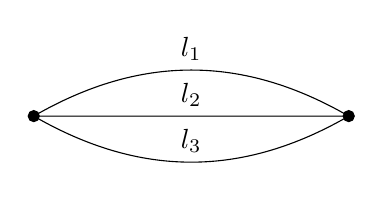
\begin{tikzpicture}
  \draw[fill=black] (0,0) circle(2pt) -- node[above]{$l_2$} (4,0) circle(2pt);
  \draw (0,0) to[out=-30,in=-150] node[above]{$l_3$} (4,0);
  \draw (0,0) to[out=30,in=150] node[above]{$l_1$} (4,0);
 \end{tikzpicture}
Denoting by $l_i$ the length of a rational chain and by $t_i$ the trend along it, balancing reduces to the following system in case (a) and (b).2:\footnote{I am not sure when this admits integral solutions, e.g. not if all $l_i$ are equal}
\[
\begin{pmatrix}
 1 & 1 & 1 \\ l_1+1 & -l_2-1 & 0 \\ l_1+1 & 0 & -l_3-1
\end{pmatrix}
\begin{pmatrix}
 t_1\\ t_2\\ t_3
\end{pmatrix}
=
\begin{pmatrix}
 1 \\ 0 \\ 0
\end{pmatrix}
\]

end{comment}

\end{enumerate}
%Say there are two special tails $T_1$ and $T_m$, intersecting $K$ at $q_1$ and $q_m$, and ordinary tails $T^\prime_1,\ldots,T^\prime_h$, meeting it at $q_1^\prime,\ldots,q_h^\prime$. Then we know from our previous computations that we need $d_K=d_{T_1}+3=d_{T_m}+3$ and $d_K=d_{T_i^\prime}+1$ for all $i$, from which we deduce that $p_1$ and $p_m$ are equidistant from the core even when they are on different rational tails, and all the other $p_i$ are further away; besides this,
%\[\omega_K(-K)(d_KK+d_{T_1}T_1+d_{T_2}T_2+\sum d_{T_i^\prime}T_i^\prime)=\omega_K(-q_1-q_m)\simeq\OO_K\]
%allows us to conclude that $q_1$ and $q_m$ have to be conjugate. In the case that $p_1$ and $p_m$ lie on the same rational tail $T$, the growth rate becomes then $4$, so that $d_K=d_T+4$ and the same computation allows us to conclude that $q$ must be Weierstrass.
\end{proof}

\begin{rem}\label{rmk:extra_conjugate}
There are two cases of stable $2$-pointed curves that arise as solutions of the balancing equation, but are not conjugate, namely:
  \begin{center}
 includegraphics[width=.8\textwidth]{extra_conjugate}  
  \end{center}
\end{rem}
\begin{comment}
\begin{lem}
 Suppose that $\pi\colon\mathcal C\to \dvr$ is a family of nodal curves over a DVR with regular total space, and that $C=\mathcal C_0$ contains a genus two subcurve $Z$ which is either a Weierstrass tail or a conjugate bridge. Then the line bundle $\mathcal L=\omega_{\mathcal C/\dvr}(D+\Sigma)$ is $\pi$-semiample, where $D$ is the effective divisor supported on $Z$ uniquely determined by Proposition \ref{prop:semistable tails}. All the conclusions of Lemma \ref{lem:general_contraction} apply.
\end{lem}
\begin{proof}
 We outline a proof in the case that $Z$ pointed by the intersection with $\overline C\setminus Z$ is stable. Note that all the multiple curves we are interested in are l.c.i.
 
 Assume first that $(Z,p)$ is irreducible and a Weierstrass tail. The desired line bundle is then $\mathcal L=\omega_{\mathcal C/\dvr}(3Z+\Sigma)$. Note that $R^1\pi_*\mathcal L(-3Z)=0$, therefore it is enough to study $\pi_*\mathcal L_{|3Z}$. There is an exact sequence:
 \[0\to\OO_{2Z}(-Z)\to\OO_{3Z}\to\OO_Z\to0\]
 which, tensored with $\mathcal L$ and using adjunction \cite[Proposition 5.73]{KolM}, gives:
 \[0\to\omega_{2Z}\to\mathcal L_{|3Z}\simeq\omega_{3Z}\to\OO_Z\to0\]
 Now, since $\pi_*\OO_Z$ has a section not vanishing along $Z$, it is enough for us to show that $H^1(\omega_{2Z})$ injects into $H^1(\omega_{3Z})$, which, by Serre duality, is equivalent to the surjectivity of $H^0(\OO_{3Z})\to H^0(\OO_{2Z})$. From the exact sequence:
 \[0\to\OO_{Z}(-2Z)\to\OO_{3Z}\to\OO_{2Z}\to0\]
 it is enough for us to show that $H^1(\OO_Z(-2Z)$ injects into $H^1(\OO_{3Z})$. Since the former has dimension $1$ over $\k$, it is equivalent to say that $H^1(\OO_{3Z})\to H^1(\OO_{2Z})$ has non-trivial kernel. But this map can be identified with the differential of the restriction map $\Pic(3Z)\to\Pic(2Z)$, which has positive-dimensional fiber by \cite[\S3.1]{Drezet} (the argument there is for a smooth underlying curve, but it seems to extend to the nodal case).
 
 Assume now that $Z$ is the union of two curves of genus one, $p\in E_1$ and $E_2$. We need to study $\mathcal L=\omega_{\mathcal C/\dvr}(3E_1+4E_2+\Sigma)$. Observe that $R^1\pi_*\mathcal L(-E_1-2E_2)=0$, therefore we can just as well study $\pi_*\mathcal L_{|E_1+2E_2}$. We have an exact sequence:
  \[0\to\OO_{2E_2}(-E_1)\to\OO_{E_1+2E_2}\to\OO_{E_1}\to 0\]
  By tensoring with $\mathcal L$ we find $\mathcal L_{2E_2}(-E_1)\simeq\omega_{2E_2}(2E_1+2E_2)\simeq\omega_{2E_2}$ (because the divisor in brackets can be written as the difference between a multiple of $\pi^*(0)$ and something supported away from a neighbourhood of $E_2$), and $\mathcal L_{E_1+2E_2}\simeq\omega_{E_1+2E_2}(-2p)$. We want the injectivity of $H^1(\omega_{2E_2})\to H^1(\omega_{E_1+2E_2}(-2p))$, which is Serre-dual to the surjectivity of $H^0(\OO_{E_1+2E_2}(2p))\to H^0(\OO_{2E_2})$. By twisting with $-2E_1-2E_2$ the exact sequence:
  \[0\to\OO_{E_1}(-2E_2)\to\OO_{E_1+2E_2}\to\OO_{2E_2}\to 0\]
  and noticing that $H^1(\OO_{E_1}(2p-2q))\simeq\k$ ($Z$ is a Weierstrass tail iff $2p\sim2q\in\Pic(E_1)$), it is enough to show that $H^1(\OO_{E_1+2E_2}(2p))\to H^1(\OO_{2E_2})$ has non-trivial kernel. By working locally around $q$, we find that  an exact sequence:
  \begin{equation}\label{eq:normalisation}
   0\to \OO_{E_1+2E_2}\to \OO_{E_1}\oplus\OO_{2E_2}\to \k^2\to 0
  \end{equation}
  If the first ring is $\k[x,y]/(xy^2)$, the second map sends $(b(y),a(x)+ya^\prime(x))$ to $(b_0-a_0,b_1-a^\prime_0)$. Twisting with $2p$, it is enough to show that
  \begin{equation}\label{eqn:su}
  H^0(\OO_{E_1}(2p))\oplus H^0(\OO_{2E_2})\to\k^2  
  \end{equation}
  is not surjective. From $2p\sim 2q$, the exact sequence:
  \[0\to \OO_{E_2}(-E_2)\to \OO_{2E_2}\to\OO_{E_2}\to 0\]
  and the local description, we see that the image of \eqref{eqn:su} is contained in the subspace $\k\oplus0$. This concludes the proof that $\pi^*\pi_*\mathcal L\to\mathcal L$ is surjective along $E_1$. As for $E_2$, tensoring with $\mathcal L$ the exact sequence
   \[0\to \OO_{E_1+E_2}(-E_2)\to \OO_{E_1+2E_2}\to\OO_{E_2}\to 0\]
   we see that it is enough to show $H^1(\omega_{E_1+E_2}(2E_1+2E_2))\hookrightarrow H^1(\omega_{E_1+2E_2}(2E_1+2E_2))$, or its Serre dual $H^0(\OO_{E_1+2E_2}(2p))\twoheadrightarrow H^0(\OO_{E_1+E_2}(2p))$, which follows from \eqref{eq:normalisation} and the usual normalisation exact sequence for the nodal curve $E_1+E_2$.
   
  Let us deal with the case that $Z$ is the union of a rational curve $p\in R$ with a genus one curve $E$ along two nodes $q_1,q_2$. We are interested in the line bundle $\mathcal L=\omega_{\mathcal C/\dvr}(3R+4E+\Sigma)$, and we find that $R^1\pi_*\mathcal L(-R-2E)=0$. Following in the steps of the previous case, the surjectivity of $\pi_*\mathcal L_{|E+2R}\to\pi_*\OO_R$ follows from the surjectivity of $H^0(\OO_{R+2E}(2p))\to H^0(\OO_{2E})$, but the latter is easily implied by $h^1(\OO_{R}(2p-2(q_1+q_2)))=0$. Similarly, the surjectivity of $\pi_*\mathcal L_{|E+2R}\to\pi_*\OO_E$ follows from comparing the ``normalisation sequences'' as in the previous paragraph. This exhausts the stable Weierstrass tails.
\end{proof}
\end{comment}

\section{The new moduli functors}\label{sec:stability}
The following generalises \cite[Definition 3.4]{SMY1}.
\begin{dfn}
 Let $(C,p_1,\ldots,p_n)$ be a reduced curve, marked by smooth points. For a nodally attached subcurve $D\subseteq C$, we define its \emph{level} as \[ \lev(D)=\lvert D\cap\overline{C\setminus D}\rvert+\lvert\{p_1,\ldots,p_n\}\cap D\rvert.\]
\end{dfn}
We say a Gorenstein curve $C$ is \emph{minimal} if it contains no node $x$ such that the normalisation of $C$ at $x$ consists of two connected components, one of which has genus zero. When $C$ has arithmetic genus one, this is the same as saying that $C$ contains no separating nodes. Recall \cite[Lemma 3.3]{SMY1}.

\begin{lem}\label{lem:min1}
 A minimal Gorenstein curve $Z$ of arithmetic genus one can be: a smooth elliptic curve; a ring of $r\geq 1$ copies of $\PP^1$; or an elliptic $m$-fold point whose normalisation is the disjoint union of $m$ copies of $\PP^1$. In any case $\omega_Z\simeq\OO_Z$.
\end{lem}

We may similarly describe minimal (sub)curves of genus two.
\begin{lem}\label{lem:min2}
 A minimal Gorenstein curve $Z$ of arithmetic genus two can be:
 \begin{enumerate}
  \item a smooth curve of genus two;
  \item the union of two minimal Gorenstein curves of genus one, $E_1$ and $E_2$, nodally separated by a (possibly empty) rational chain $R$;
  \item the union of a minimal Gorenstein curve of genus one $E$, and a (possibly empty) rational chain $R$, along two distinct nodes;
  \item the union of two copies of $(\PP^1,0,1,\infty)$ with three (possibly empty) rational chains $R_0, R_1, R_\infty$ joining the homonymous points;
  \item\label{case:twice1} an elliptic $m$-fold point $x$ whose normalisation is the disjoint union of either $m-1$ copies of $\PP^1$ (i.e. two branches of $x$ coincide), or $m-1$ copies of $\PP^1$ and a minimal Gorenstein curve of genus one (i.e. $Z$ contains two genus one subcurves sharing a branch);
  \item\label{case:2} or a singularity of genus two with $m$-branches, whose normalisation is the disjoint union of $m$ copies of $\PP^1$.
 \end{enumerate}
%In all cases there exists a unique $\mathfrak g^1_2$. In cases \eqref{case:twice1} and \eqref{case:2}, given a smooth point $p$ lying on a special branch, there exists a unique point $\bar p$ (possibly equal to $p$), such that $\omega_Z\simeq\OO(p+\bar p)$.
\end{lem}
\begin{rem}\label{rem:special}
In both cases \eqref{case:twice1} and \eqref{case:2} there are special branches supporting the degree of $\omega_Z$ (compare with Definition \ref{def:special_branches} and Corollary \ref{cor:deg_dualising}; recall that the restriction of the dualising sheaf to a component introduces a twist by the conductor ideal, see Noether's formula \cite[Proposition 1.2]{Catanese}). Notice that the notion of conjugate points is not always intrinsic to the curve.\end{rem}

Similarly to \cite[Corollary 3.2, Lemma 3.5]{SMY1} we can prove the following.
\begin{lem}
 Let $(C,p_1,\ldots,p_n)$ be a pointed \emph{semistable} curve of arithmetic genus two, with minimal genus two subcurve $Z$. For every subcurve $Z^\prime\subseteq C$ of genus two, we have an inclusion $Z\subseteq Z^\prime$ and $\lev(Z)\leq\lev(Z^\prime)$.
\end{lem}

We finally come to the definition of $m$-stability for curves of genus two.
\begin{dfn}\label{def:m-stability}
 Fix positive integers $m<n$. Let $(C,p_1,\ldots,p_n)$ be a connected, reduced, complete curve of arithmetic genus two, marked by smooth distinct points. We say that $C$ is $m$-stable if:
 \begin{enumerate}[leftmargin=.7cm]
  \item\label{cond:sing} $C$ is Gorenstein with only: nodes; elliptic $l$-fold points, $l\leq m+1$; type $I_{\leq m}$, type $I\!I_{\leq m}$, and dangling $I\!I_{m+1}$ singularities of genus two, as singular points.
  \item\label{cond:lev2} If $Z$ is a connected subcurve of arithmetic genus two, then $\lev(Z)>m$.
  \item\label{cond:lev1} If $E$ is a nodally attached subcurve of arithmetic genus one, $\lev(E)>m+1$.
  \item\label{cond:aut} $H^0(C,\Omega_C^\vee(-\sum_{i=1}^n p_i))=0$.
  \item\label{cond:p1} If $C$ contains a singularity of genus two, or an elliptic $l$-fold with a self-branch, $p_1$ is connected (through a rational chain) to one of the special branches (see Remark \ref{rem:special}). If $C$ contains two genus one subcurves sharing a branch, and $E_1$ has level less than $m+2$, then $p_1$ is connected to $E_1$.
 \end{enumerate}
\end{dfn}

\begin{rem}
 The definition is not $\mathfrak{S}_n$-symmetric. In the arguments below, we exploit the asymmetry to write the dualising line bundle of a genus two (sub)curve $Z$ as $\omega_Z\simeq\OO_Z(q_1+\bar q_1)$, where $q_1$ is the point of $Z$ closest to $p_1$, and $\bar q_1$ its conjugate, possibly depending on a one-parameter smoothing. Compare with the situation in genus one, where the dualising line bundle of a minimal Gorenstein curve is trivial (all smooth points are non-special).
\end{rem}

\begin{rem}\label{rmk:lev1solev2}
 If there is a subcurve of genus one, condition \eqref{cond:lev1} and condition \eqref{cond:aut} jointly imply condition \eqref{cond:lev2}. Indeed, from Corollary \ref{cor:explicitnoaut} we see that $\lev(Z)\geq\lev(E)-1$. The only cases (up to relabelling) in which the level drops by one are: when $Z=(E,p_1,\ldots,p_{l-2},q_1,q_2)\sqcup_{\{q_1,q_2\}}(\PP^1,q_1,q_2,p_{l-1})$; and when $Z=(E_1,p_1,\ldots,p_{l-1},q)\sqcup_q(E_2,q)$, where all the $E$ have genus one.
\end{rem}


\begin{lem}[boundedness]
 If $(C,p_1,\ldots,p_n)$ is an $m$-stable curve of genus two, the $N$-th power of $A=\omega_C(\sum_{i=1}^np_i)$ is very ample for every $N>2+8(m+1)$.
\end{lem}
\begin{proof}
 It is enough to show that, for every pair of points $p,q\in C$ (possibly equal):
 \begin{enumerate}
  \item \emph{basepoint-freeness}: $H^1(C,A^{\otimes N}\otimes I_p)=0$;
  \item \emph{separating points and tangent vectors}: $H^1(C,A^{\otimes N}\otimes I_pI_q)=0$.
 \end{enumerate}
By Serre duality we may equivalently show that $H^0(C,\omega_C\otimes A^{-N}\otimes(I_pI_q)^\vee)=0$. Let $\nu\colon\tilde C\to C$ be the normalisation, and let $\nu^{-1}(p)=\{p_1,\ldots,p_h\}$, $\nu^{-1}(q)=\{q_1,\ldots,q_k\}$, with $h,k\leq m+1$. It follows from Proposition \ref{prop:classification} (and \cite[Proposition A.3]{SMY1}) that $\nu_*\OO_{\tilde C}(-D)\subseteq I_pI_q$ for $D=4(\sum_{i=1}^hp_i+\sum_{j=1}^kq_j)$ (note that $\deg(D)\leq 8(m+1)$); furthermore, the quotient is torsion, therefore, by applying $\hhom(-,\OO_C)$ and adjunction, we find $(I_pI_q)^\vee\subseteq\nu_*\OO_{\tilde C}(D)$. It is thus enough to show that $H^0(\tilde C,\OO_{\tilde C}(D)\otimes\nu^*(\omega_C\otimes A^{-N}))=0$. Finally, $\nu^*\omega_C$ has degree at most two, and $\nu^*A$ has degree at least one on any branch of $\tilde C$, hence it is enough to take $N>2+8(m+1)$.
\end{proof}

\begin{lem}[deformation openness]
 Let $(\mathcal C,\sigma_1,\ldots,\sigma_n)\to S$ be a family of curves over a Noetherian base scheme with $n$ sections. The locus \[\{s\in S|(\mathcal C_{\bar s},\sigma_1(\bar s),\ldots,\sigma_n(\bar s)) \text{ is } m\text{-stable}\}\] is Zariski-open in $S$.
\end{lem}
\begin{proof}
 Having connected fibers which are Gorenstein curves of arithmetic genus two is an open condition (see for example \cite[\href{https://stacks.math.columbia.edu/tag/0E1M}{Tag 0E1M}]{stacks-project}). Only singularities of genus zero (nodes), one (elliptic $l$-folds), and two may then occur.
 
 The case $m=1$ deserves special attention. In this case, that condition \eqref{cond:sing} is open follows from acknowledging that $I_1=A_4$, $I\!I_2=A_5$, while tacnodes, cusps, and nodes are $A_3$, $A_2$, and $A_1$-singularities respectively, and from Grothendieck's results on the deformation theory of ADE singularities (see Theorem \ref{thm:ADE} above).
 
 The case $m\geq 2$ simply follows from upper semicontinuity of embedded dimension and the fact that we have exhausted all possible Gorenstein singularities of genus $\leq 2$, and embedding dimension $\leq m+1$.
 
 Condition \eqref{cond:aut} translates to: the locus where the automorphism group is unramified is open in the base. Homogeneity can be used to prove that being unramified, which is open in the source, is also open in the target, for the structural morphism of a group scheme; see the end of the proof of \cite[Lemma 3.10]{SMY1}.
 
 The other conditions are topological, hence constructible. With Noetherian assumptions, it is enough to check their openness over the spectrum of a discrete valuation ring. Assume that the geometric generic fiber $C_{\bar\eta}$ contains two genus one subcurve $E_{1,\bar\eta}$ and $E_{2,\bar\eta}$; their closures $E_1$ and $E_2$ in $\mathcal C$ are then flat families of genus one curves over $\dvr$. If $E_{1,\bar\eta}$ and $E_{2,\bar\eta}$ are disconnected, then so are $E_1$ and $E_2$, by local constancy of the number of connected components (from the Zariski decomposition and \cite[\href{https://stacks.math.columbia.edu/tag/0E0D}{Tag 0E0D}]{stacks-project}). If $E_{1,\bar\eta}$ and $E_{2,\bar\eta}$ are joined by a disconnecting node $q_{\bar\eta}$, then so are $E_{1,0}$ and $E_{2,0}$; indeed, the unique limit of $q_{\bar\eta}$ must be a singular point of the projection, but cannot be any worse than a node (because we have already exhausted all the available genus). Finally, if $E_{1,\bar\eta}$ and $E_{2,\bar\eta}$ share a branch, then so do $E_{1,0}$ and $E_{2,0}$; on the other hand, if $E_{i,\bar\eta}$ has more than one branch, then so does $E_i$. Similarly, if $C_{\bar\eta}$ contains only one subcurve of genus one, with two nodes joined by a rational chain, so does $C_0$. The upshot of this discussion is that
 \[\lvert E_{i,\bar\eta}\cap\overline{C_{\bar\eta}\setminus E_{i,\bar\eta}}\rvert=\lvert E_{i,0}\cap\overline{C_{0}\setminus E_{i,0}}\rvert.\]
 The number of markings on $E_i$ is also constant. Hence we can deduce condition \eqref{cond:lev1} for $C_{\bar\eta}$ from the same condition on $C_0$. Condition \eqref{cond:lev2} follows in this case from Remark \ref{rmk:lev1solev2}; it can be proved analogously when there is no subcurve of genus one.
 
 Finally, suppose that $C_{\bar\eta}$ has a genus two singularity, then so does $C_0$. The (union of the) distinguished branch(es) $E_{\bar\eta}$ of $C_{\bar\eta}$ is a genus one singularity, and so is its limit $E_0$ in $C_0$. It has to contain the distinguished branch(es) of $C_0$, because any subcurve not containing them has genus zero; therefore, by assumption, $E_0$ contains $p_{1,0}$. Then also $E_{\bar\eta}$ contains $p_{1,\bar\eta}$, because the markings are contained in the non-singular locus of the curve. Similarly, $C_{\bar\eta}$ has a genus one singularity with a self-branch, the limit of such a branch is a genus one subcurve $E_0$ of $C_0$; the latter may very well acquire a genus two singularity, but $E_0$ will contain the special branches of it, so it will be connected to $p_1$. We conclude as above. The case that $C_{\bar\eta}$ contains a genus one subcurve of low level is analogous. We have thus proved that condition \ref{cond:p1} is open.
\end{proof}

\begin{dfn}
 We shall denote by $\oM^{(m)}_{2,n}$ the moduli functor of $n$-pointed $m$-stable curves of genus two.
\end{dfn}

It follows from the previous lemmas and standard arguments that $\oM^{(m)}_{2,n}$ is represented by a Deligne-Mumford stack of finite type.

\begin{prop}[Valuative criterion of properness for $\oM^{(m)}_{2,n}$]
 Given a smooth $n$-pointed curve of genus two $C_\eta$ over a discrete valuation field $\eta=\operatorname{Spec}(K)\hookrightarrow\dvr$, there exists a finite base-change $\dvr^\prime\to\dvr$ after which $C_\eta$ can be completed to an \emph{$m$-stable} curve over $\dvr^\prime$. Two such models are always dominated by a third one.
\end{prop}
\begin{proof}
 \emph{Existence of limits.}
  We start with a smooth $n$-pointed curve of genus two over a discrete valuation field. By the semistable reduction theorem \cite[Corollary 2.7]{DM}, we may find a finite base-change $\dvr^\prime\to\dvr$ and a semistable curve $\mathcal C^\prime\to\dvr^\prime$ with regular total space, such that its generic fiber is isomorphic to the pullback of the curve we started with. By Castelnuovo's criterion, we may further assume that the central fiber contains no rational tails.
  
  We check whether $p_1$ is Weierstrass or not: in the former case, change base with $\pi^{\prime\prime}\mapsto(\pi^\prime)^3$ and resolve; in the latter, mark $\mathcal C^\prime$ with an extra section $\bar p_1$ given by the closure of the conjugate point $\bar p_1(\eta)$ (unless it coincides with one of $p_1,\ldots,p_n$; if it coincides with $p_1$, we have a Weierstrass point indeed), then change base with $\pi^{\prime\prime}\mapsto(\pi^\prime)^2$ and resolve. We drop the primes from notation. $\mathcal C_0$ is now marked with a(n extra) smooth point $\bar p_1$. The base-change is a technical expedient we find useful in the forthcoming construction.
  
  We claim there is a unique genus two subcurve $Z$ of $\mathcal C_0$ that satisfies the shape requirements of Proposition \ref{prop:tailI} (resp. \ref{prop:tailII}) - or consists of two disjoint balanced subcurves of genus one - guaranteeing the curve we obtain by contracting $Z$ has bounded above singularities and bounded below level as in conditions \eqref{cond:sing},\eqref{cond:lev2}, and \eqref{cond:lev1} of Definition \ref{def:m-stability}.
  
  We think of this process as drawing a family of expanding circles on the dual graph (except, they are neither exactly circles, nor always expanding). Note that we may at any point blow-up the curve at a marking on the central fiber, and consider the strict transform of the corresponding section; thus markings can effectively be considered as infinite legs in the dual graph. We are going to contract the strict interior of the circle; note that the number of branches of the resulting singularity is determined by the inner valence of the circle, and the level by the outer valence.
  
  For simplicity, we start by examining the case that the core of $\mathcal C_0$ is irreducible, and $p_1$ is Weierstrass. Step $0$: if the core $K$ has level $\geq m+1$, then the curve is already $m$-stable. Otherwise, draw a first circle comprising $K$, and reaching every second closest rational component along any rational tree attached to $K$, except for the tree containing $p_1$. Note that the inner valence is exactly $\lev(K)$, thanks to the base-change we have performed earlier, and in particular it is no larger than $m$; on the other hand, semistability implies that the outer valence is non-decreasing - it is important to consider markings as infinite legs for this -: if it is $\geq m+1$ we stop, otherwise we repeat the process. Calling $K_1$ the union of the components strictly inside the first circle, $\mathcal C_0$ is the union of $K_1$ and a number of rational trees; if the outer valence at the first step is still $\leq m$, we enlarge the circle by reaching one step further along the rational tree containing $p_1$, and three steps along all the other ones. Because a circle of very large radius has both inner and outer valence equal to $n>m$, by increasing the radius step by step we will eventually reach level $m+1$ or higher. If we stop at the $l$-th step, the line bundle we will use to perform the contraction is
  \begin{multline*}
  \mathcal L=\omega_{\mathcal C/\dvr}(3l K + \sum_{R\in [p_1,K]}[3l-3\dist(R,K)]_+R +\sum_{R\notin T_1}[3l-\dist(R,K)]_+R +\\
  \sum_{R\in T_1,R\notin [p_1,K]}[3l-3\dist(T_1\wedge T_R,K)-\dist(R,T_1\wedge T_R)]_+R+ \sum_{i=1}^np_i)
  \end{multline*}
  where $T_1$ is the rational tree (connected component of $\mathcal C_0\setminus K$) containing $p_1$, $T_R$ the one containing $R$, $T_1\wedge T_R$ their common component furthest from the core, $\dist$ is the distance on the dual graph, and $[k]_+=\max\{0,k\}$ for any integer $k$. If $\mathcal L$ differs from $\omega_{\mathcal C/\dvr}^{\text{log}}$ by a vertical divisor whose support is $Z$, the shape prescription being satisfied by construction, it follows from Proposition \ref{prop:contractionI} that $\mathcal L$ is $\pi$-semiample, and the contraction it yields contains a singularity of type I with $p_1$ cleaving to the special branch. Note that $\mathcal L$ contracts as well the semistable rational components that are disjoint from $Z$, hence the resulting curve has no (infinitesimal) automorphisms. The level condition is satisfied by construction, therefore $\overline{\mathcal C}_0$ is $m$-stable.
  
  The case that the core is irreducible and $p_1$ is not Weierstrass is dealt with in a similar fashion. Remember that in this case we have constructed a conjugate section $\bar p_1$; this is an auxiliary marking that will be forgotten in the end, and should not be taken into account when computing the level. At every step we draw a larger circle by including one more component along the trees containing $p_1$ and $\bar p_1$, and two more along every other tree; the inner valence of the new circle is the same as the outer valence of the old one, thanks to the $2:1$ base-change. At the $l$-th step we are going to use the line bundle
  \begin{multline*}
  \mathcal L=\omega_{\mathcal C/\dvr}(2l K + \sum_{\substack{R\in [p_1,K]\\ \text{ or }[\bar p_1,K]}}[2l-2\dist(R,K)]_+R +\sum_{R\notin T_1,\bar T_1}[2l-\dist(R,K)]_+R +\\
  \sum_{\substack{R\in T_1,R\notin [p_1,K]\text{ or} \\ R\in \bar T_1,R\notin [\bar p_1,K]}}[2l-2\dist(T_1\wedge T_R,K)-\dist(R,T_1\wedge T_R)]_+R+ \sum_{i=1}^np_i+\bar p_1)
  \end{multline*}
  to contract the strict interior of the circle. It follows from Proposition \ref{prop:contractionII} that $\mathcal L$ is $\pi$-semiample, and the associated contraction contains a singularity of type II with $p_1$ cleaving to one of the twin branches. Note that a $I\!I_{m+1}$ singularity will occur only if the level is $m$ and $\bar p_1$ does not coincide with any other special point, so that one of the twin branches remains dangling after forgetting $\bar p_1$. Again, the stability condition is satisfied by construction.
  
  \smallskip
  
  Suppose next that the minimal subcurve of genus two $Z$ contains two subcurves of genus one; call $E_1$ and $E_2$ the minimal such, and assume that $p_1$ cleaves to $E_1$ in a point that is $2$-torsion with respect to the node separating $E_1$ from $E_2$. We start by drawing expanding circles around $E_2$ until the level condition for it is satisfied, and then we do the same for $E_1$, so that \eqref{cond:p1} holds; observe, though, that as soon as the two circles touch, the contraction will not have two distinguished genus one subcurves anymore, therefore we need to check \eqref{cond:lev2} rather than \eqref{cond:lev1}.
  \begin{itemize}[leftmargin=.4cm]
  \item If $\lev(E_2)\geq m+2$ is attained before the circle around $E_2$ gets to touch $E_1$, take the next $l_2\equiv 2  \pmod 3$ (thus ``undoing'' the $3:1$ base-change, which was unnecessary in this case), then contract the inner disc by the line bundle \[\mathcal L_2=\omega_{\mathcal C/\dvr}((l_2+1)E_2+\sum [l_2+1-\operatorname{dist}(E_2,R)]_+R+\sum_{i=1}^n p_i).\] Smyth's contraction lemma \cite[Lemma 2.13]{SMY1} applies, so that $E_2$ is contracted to an elliptic $l$-fold point $q_2$ ($l\leq m+1$). Consider now $E_1$. If $\lev(E_1)\leq m+1$, start drawing expanding circles around it. Either level $\geq m+2$ can be reached before touching the singularity at $q_2$, or, by contracting the maximal balanced subcurve of genus one containing $E_1$ and not $q_2$, we produce a curve having two genus one singularities that share a branch. Note that $p_1$ cleaves to the only genus one subcurve that may have level $\leq m+1$.
  \item Otherwise, one step before including $E_1$, we may contract the disc around $E_2$ to yield a genus one singularity with a genus one branch. If $\lev_2\leq m$ at this point, we need to contract the whole genus two subcurve. What happens at this critical step is that the multiplicity of $D$ along $E_1$ grows from $0$ to $3$, hence $D$ will be supported three steps further along each rational tail departing from $E_2$. Because the critical step is $\equiv 1\pmod 3$, the length of the rational tails is and remains $\equiv 2 \pmod 3$, hence we perform only one ``meaningful'' step forward (i.e. on the original central fiber, before changing base), thanks to the preliminary base-change. See Figure \ref{fig:critical}. In particular, the inner valence of the disc will be $\leq m$.
  \begin{figure}
   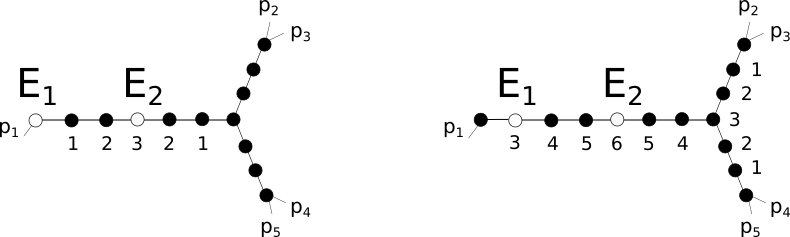
\includegraphics[width=.8\textwidth]{critical_step}
   \caption{An instance of the critical step, when we pass from contracting the two genus one subcurves separately, to contracting the genus two subcurve as a whole. On the left, the contraction produces a tacnode with a genus one branch, having $\lev_2=3$. On the right, the contraction produces a singularity of type $I_3$. Note that in the meantime we performed a blow-up at $p_1$.}\label{fig:critical}
  \end{figure}
 We may now proceed as in the irreducible case, expanding the circle at every step by $1$ along $T_1$ and by $3$ along all other rational tails.
 \end{itemize}
 The case that the central fiber contains two subcurves of genus one, and $p_1$ cleaves to a non-Weierstrass point, is analogous: it is enough to replace the number $3$ by the number $2$, and $2$ by $1$, in the previous argument. The only novelty is, it can happen that $p_1$ is equidistant from $E_1$ and $E_2$, cleaving to the rational chain joining them. In this case we start by expanding a circle around the one with the lowest level; if they have the same level, expand them simultaneously. If at a later stage $p_1$ becomes closer to one of the two circles, proceed as above.
 
 \smallskip
 
 When the core consists of an elliptic curve $E$ with a rational bridge $R$, and $p_1$ cleaves to a Weierstrass point - either on $E$ or on $R$ -, we have noticed above (see the end of Remark \ref{rmk:Wandconj}), that $R$ comprises an odd number $k=2h+1$ of rational components. We start as above by enlarging a balanced circle around $E$ in order to establish the level condition \eqref{cond:lev1}; once again there is a critical step (after which we contract a genus two subcurve, and check \eqref{cond:lev2} instead) when the circle touches itself along $R$, and we observe that this happens after the $(3h+2)$-th step, therefore extending the circle by $1$ along the tail containing $p_1$, and by $3$ on all the other ones, only makes one meaningful step. The case of a non-Weierstrass point on the elliptic bridge is analogous.
 
 \smallskip
 
 Finally, the case that the central fiber has geometric genus zero is dealt with as if the core was irreducible, since we do not introduce any genus zero singularity other than the node (the remaining ones are not Gorenstein).

  \begin{comment}
  Now check whether $p_1$ afferes to a Weierstrass point or not: in the former case, change base with $\pi^{\prime\prime}\mapsto(\pi^\prime)^3$, in the latter with $\pi^{\prime\prime}\mapsto(\pi^\prime)^2$; then resolve. This has the effect of replacing every node with a chain of two (resp. one) $-2$-curve. It is a technical expedient we find useful in the construction. We drop the primes from notation.
  
  Next we identify a (not necessarily connected) subcurve that needs be contracted in order to find the $m$-stable limit. The process can be thought of as drawing expanding circles on the dual graph (except, they are not always expanding). We may at any point blow-up the curve at a marking on the central fiber, and consider the strict transform of the corresponding section; thus markings can effectively be considered as legs going to infinity in the dual graph.
  
  We start from the case that the core $Z$ is irreducible. Suppose that the level of $Z$ is $l\leq m$; then we may contract (a subcurve containing) $Z$ as follows. Let $q_1$ the point of $Z$ closest to $p_1$.
 \begin{enumerate}
  \item\label{caseW} If $(Z,q_1)$ is Weierstrass, call $S_h$ the $-2$-curves closest to $\tilde Z$, and $R_h$ the second closest. Consider the line bundle
  \[\mathcal L_{j+1}=\omega_{\mathcal B_{j+1}/\dvr}(3\tilde Z+2\sum_{h=1}^{l_j-1}S_h+\sum_{h=1}^{l_j-1}R_h+\tilde \sigma_{1,j}+\ldots+\tilde\sigma_{n,j}).\]
  By the contraction lemma \ref{lem:contraction}... By the classification of semistable tails, $\mathcal C_{j+1,0}$ acquires a singularity of type $I\!I\!I_{l}$ (which works out by our initial choice of base-change), and $p_1$ is connected to the singular branch.
  \item\label{casenW} If $(Z,q_1)$ is not Weierstrass, call $R_h$ the $-2$-curves closest to $\tilde Z$. In case there is no rational tail attached to $\bar q_1$, blow up the latter point. Consider then the line bundle
  \[\mathcal L_{j+1}=\omega_{\mathcal B_{j+1}/\dvr}(2\tilde Z+\sum_{h=1}^{l_j-1}R_h+\tilde \sigma_{1,j}+\ldots+\tilde\sigma_{n,j});\]
  By the contraction lemma \ref{lem:contraction}... By the classification of semistable tails, $\mathcal C_{j+1,0}$ acquires a singularity of type $I\!I_{l}$ or $I\!I_{l+1}$ (in which case one of the twin branches is dangling), and $p_1$ is connected to one of the twin branches.
 \end{enumerate}
 More generally, in case \ref{caseW} we may draw circles around $Z$ that at each step expand by $1$ along the tail containing $p_1$ and by $3$ along all other tails. Note that at each step the number of branches is the same as the level one step before that thanks to our base-change choice. If $l$ denotes the radius of the circle along $T_1$, the line bundle
 \[\omega_{\mathcal C}\left(3lZ+\sum_{R_i\in T_1}3(l-\operatorname{dist}(R_i,Z))R_i+\sum_{R_i\not\in T_1}(l-\operatorname{dist}(R_i,Z))R_i+\sigma_1+\ldots+\sigma_n\right)\]
 performs the desired contraction.
  
 Suppose the minimal subcurve of genus two $Z$ contains two subcurves of genus one; call $E_1$ and $E_2$ the minimal such, and assume that $p_1$ afferes to $E_1$. Start drawing circles around $E_2$. If $E_2$ already has level bigger than $m+1$, stop with the circle of radius $0$. Otherwise grow the radius by $1$ at a time. The curve to be contracted is the inner disk, so the number of branches is measured by the vertices lying on the circle, and the level by the number of exciding edges. Both are non-decreasing with the radius. We exmine the Weierstrass case; the conjugate is entirely analogous. Note that at this stage we perform one meaningful step every three, due to our choice of base-change.
  \begin{enumerate}
   \item If level $\geq m+2$ is reached before the circle touches $E_1$, take the next possible $\equiv 2\mod 3$ radius, then contract the inner circle by the line bundle
   \[ \omega_{\mathcal C}((l_2+1)E_2+\sum_i \max(l_2+1-\operatorname{dist}(E_2,R_i),0)R_i\oplus\sigma_1\oplus\ldots\oplus\sigma_n)\]
   where $l_2$ is the radius of the circle around $E_2$. Consider now $E_1$: if $\lev(E_1)\leq m+1$ start expanding the circle around it. Again, either level $\geq m+2$ can be reached before touching $E_2$, or, by contracting the maximal balanced subcurve of genus one containing $E_1$, we produce a curve having two genus one singularities that share a branch. Notice that in this case $p_1$ afferes to the only genus one subcurve that may have level $\leq m+1$.
   \item Otherwise, one step before reaching $E_1$, we may contract to produce a genus one singularity with a genus one branch. If the level is $\leq m$ at this point, consider the genus two subcurve $Z$ as a whole. Observe that the line bundle we would like to consider at this point starts with weight $3$ instead of $1$ along the tail connecting $p_1$ to $E_1$. This means that it will be supported two steps further along each rational tail departing from $Z$ except the tail containing $p_1$. Note also that getting to include $E_2$ happens at a step $\equiv 0 \mod 3$, therefore including two more components on each rational tail will not make the number of branches grow above $m$. We may now continue as before, at every step expanding the circle by $1$ along $T_1$ and by $3$ along all other rational tails.
  \end{enumerate}
 In case $p_1$ is equidistant from $E_1$ and $E_2$ (it must then affere to the rational chain joining them), start by expanding a circle around the one with lower level; if they have the same level, expand them simultaneously. If at a later stage $p_1$ becomes closer to one of the two circles, proceed as above.
 
 
 
 
 
 
  We start with a smooth $n$-pointed curve of genus two over a discrete valuation field. By the semistable reduction theorem \cite[Corollary 2.7]{DM}, we may find a finite base-change $\dvr^\prime\to\dvr$ and a semistable curve $\mathcal C^\prime\to\dvr^\prime$ with regular total space, such that its generic fiber is isomorphic to the pullback of the curve we started with. By Castelnuovo's criterion, we may further assume that the central fiber contains no rational tails. We drop the prime from our notation.
 
 We may construct a zigzag diagram of birational morphisms of curves over $\dvr$, never altering the generic fiber:
 \bcd
 & \mathcal B_1\ar[dl,"p_1"]\ar[dr,"q_1"] & & \mathcal B_2\ar[dl,"p_2"] & \ldots & \mathcal B_{t-1}\ar[dr,"q_{t-1}"] & & \mathcal B_{t}\ar[dl,"p_{t}"]\ar[dr,"q_{t}"] & \\
 \mathcal C_0:=\mathcal C\ar[rr,dashed] & & \mathcal C_1\ar[r,dashed] & {} & \ldots & {}\ar[r,dashed] & \mathcal C_{t-1}\ar[rr,dashed] & & \mathcal C_t
 \ecd
 such that:
 \begin{enumerate}[label=(\roman*)]
  \item $\mathcal C_i\to\dvr$ is a Gorenstein curve of genus two, with $n$ smooth sections $\sigma_{1,i},\ldots,\sigma_{n,i}$;
  \item\label{cond:regnodes} the total space of $\mathcal C_i$ is regular at the nodes of $\mathcal C_{i,0}$;
  \item every nodally attached rational component of $\mathcal C_i$ has at least two special points;
  \item if $\mathcal C_i$ contains two subcurves of genus one, then so do all $\mathcal C_j, j\leq i$ and their minimal level sequence is non-decreasing; on the other hand, if $\mathcal C_i$ contains only subcurve of genus one, then so do all $\mathcal C_j, j\leq i$, and their minimal level sequence is non-decreasing;
  \item the level of a minimal subcurve of genus two is non-decreasing;
  \item $\mathcal C_t$ contains a genus two singularity and no disconnecting nodes.
 \end{enumerate}
 Here is the procedure:
 \begin{enumerate}
  \item\label{twogenusone} If the special fiber $\mathcal C_{i,0}$ contains two \emph{disjoint} subcurves of genus one, let $E_1$ and $E_2$ be the minimal such. Let $\mathcal B_{i+1}$ be the blow-up of $\mathcal C_i$ in the points $\{\sigma_{1,i},\ldots,\sigma_{n,i}\}\cap(E_1\cup E_2)$; these are smooth points of $\pi_i$, thus $\mathcal C_i$ is regular near them. Denote the strict transform of $\cdot$ by $\tilde{\cdot}$. $\tilde E_1$ and $\tilde E_2$ are nodally attached, hence Cartier by assumption \ref{cond:regnodes}. We may therefore consider the line bundle
  \[\mathcal L_{i+1}=\omega_{\mathcal B_{i+1}/\dvr}(\tilde E_1+\tilde E_2+\tilde \sigma_{1,i}+\ldots+\tilde\sigma_{n,i}),\]
  which is: trivial along $\tilde E_1$, $\tilde E_2$ (by adjunction and Lemma \ref{lem:min1}), and every rational tail with only two special points, except those adjacent to either $\tilde E_1$ or $\tilde E_2$; ample everywhere else. Let \[\mathcal C_{i+1}=\Proj_\dvr\pi_{\mathcal B_{i+1},*}\left(\bigoplus_{n=0}^\infty \mathcal L_{i+1}^{\otimes n}\right).\]
  By the contraction lemma \ref{lem:contraction}...
  \item\label{onegenusone} Similarly, if the special fiber $\mathcal C_{i,0}$ contains only one subcurve of genus one, which is nodally joined to itself through a rational chain, let $E$ be the minimal such subcurve. $\mathcal B_{i+1}$ is obtained by blowing up $\mathcal C_i$ in the regular points $\{\sigma_{1,i},\ldots,\sigma_{n,i}\}\cap E$. The line bundle
  \[\mathcal L_{i+1}=\omega_{\mathcal B_{i+1}/\dvr}(\tilde E+\tilde \sigma_{1,i}+\ldots+\tilde\sigma_{n,i})\]
  is again trivial on $E$ and every rational tail with only two special points, except those adjacent to $\tilde E$; ample averywhere else.
 \end{enumerate}
 Notice that the number of rationally attached rational components strictly decreases at every step, hence after finitely many steps we reach the following situation: the two genus one subcurves have a common node or branch (case \ref{twogenusone}), or the only subcurve of genus one has either two branches that meet in a node, or two coinciding branch. Under these conditions, we pass to considering the minimal genus two subcurve as a whole. At this point - or if there was no genus one subcurve to start with -, proceed as follows. Let $Z$ be the minimal subcurve of genus two in $\mathcal C_{j,0}$; let $q_1$ the point of $Z$ closest to $p_1$.
 \begin{enumerate}
  \item If $(Z,q_1)$ is Weierstrass, let $\mathcal B_{j+1}$ be obtained as the blow-up of $\mathcal C_j$ at $q_1$, ``three times'' at all the (other) points $\{\sigma_{1,j},\ldots,\sigma_{n,j}\}\cap Z$ (if $p_1\in Z$), and ``twice'' at all the (other) nodes of $\mathcal C_{j,0}$ such that one of their branches is in $Z$, and the other is not (if $q_1\neq p_1$). Call $S_h$ the exceptional divisors closest to $\tilde Z$, and $R_h$ the second closest. Consider then the line bundle
  \[\mathcal L_{j+1}=\omega_{\mathcal B_{j+1}/\dvr}(3\tilde Z+2\sum_{h=1}^{l_j-1}S_h+\sum_{h=1}^{l_j-1}R_h+\tilde \sigma_{1,j}+\ldots+\tilde\sigma_{n,j});\]
  it is indeed a line bundle, again by assumption \ref{cond:regnodes}. By the contraction lemma \ref{lem:contraction}... By the classification of semistable tails, $\mathcal C_{j+1,0}$ acquires a singularity of type $I\!I\!I_{l_i}$, and $p_1$ is connected to the singular branch.
  \item If $(Z,q_1)$ is not Weierstrass, blow up $\mathcal C_j$ at $q_1$ and at the point of $Z$ which is conjugate to $q_1$; let $\mathcal B_{j+1}$ be obtained by further blowing up $\mathcal C_j$ ``twice'' at all the (other) points $\{\sigma_{1,j},\ldots,\sigma_{n,j}\}\cap Z$ (if $p_1\in Z$), and only once at all the (other) nodes of $\mathcal C_{j,0}$ such that one of their branches is in $Z$, and the other is not (if $q_1\neq p_1$). Call $R_h$ the exceptional divisors closest to $\tilde Z$. Consider then the line bundle
  \[\mathcal L_{j+1}=\omega_{\mathcal B_{j+1}/\dvr}(2\tilde Z+\sum_{h=1}^{l_j-1}R_h+\tilde \sigma_{1,j}+\ldots+\tilde\sigma_{n,j});\]
  it is indeed a line bundle, again by assumption \ref{cond:regnodes}. By the contraction lemma \ref{lem:contraction}... By the classification of semistable tails, $\mathcal C_{j+1,0}$ acquires a singularity of type $I\!I_{l_i+1}$, and $p_1$ is connected to one of the twin branches.
 \end{enumerate}
 Notice again that the number of rationally attached rational components strictly decreases at every step, hence after finitely many steps we obtain $\mathcal C_{t,0}=Z$ and there are no disconnecting nodes.\end{comment}
 \medskip
 
 \emph{Uniqueness of limits.} By the semistable reduction theorem, there is a diagram
 \bcd
 & \mathcal C^{ss}\ar[ld,"\phi" above]\ar[dr,"\phi^\prime" above] & \\
 \mathcal C\ar[dr] & & \mathcal C^\prime\ar[dl] \\
 & \dvr &
 \ecd
 extending the isomorphism between the generic fibers, where $\mathcal C^{ss}$ has semistable central fiber and regular total space.
 
 \textbf{Claim 1:} If $\mathcal C^\prime_0$ has only singularities of genus $\leq i$ ($i=0,1$), then so does $\mathcal C_0$.
 
 \noindent First, assume that $\mathcal C^\prime_0$ has only nodes. If $\mathcal C_0$ has a singular point $x$ of genus one, $E:=\phi^{-1}(x)$ is an \emph{unmarked} subcurve of arithmetic genus one and level $\leq m+1$ of $\mathcal C^{ss}_0$. Then so is $\phi^\prime(E)$: indeed, $\phi^\prime$ being a contraction, it has connected fibers, which excludes the possibility that $\phi^\prime$ lowers the genus of $E$ by realising a finite cover of a line. This contradicts the $m$-stability of $\mathcal C^\prime$. We may argue similarly if $x$ is a genus two singularity with $\leq m$ branches. On the other hand, if $x$ is dangling $I\!I_{m+1}$, there is a $-1$-curve $R$ adjacent to $\phi^{-1}(x)$; $\phi^\prime$ must contract $R$ by DM stability of $\mathcal C^\prime$, hence $\phi^\prime(\phi^{-1}(x))$ is again a genus two curve of level $\leq m$.
 
 Assume now that $\mathcal C^\prime_0$ has at worst singularities of genus one, while $\mathcal C_0$ has a singularity $x$ of genus two; the case of a dangling $I\!I_{m+1}$ can be excluded as above. Then $\mathcal C^{ss}_0=Z\cup R_1\cup \ldots\cup R_l$, with $Z=\phi^{-1}(x)$ and $l\leq m$. If $Z$ has geometric genus two, or is irreducible of geometric genus one, $\phi^\prime(Z)$ violates the $m$-stability of $\mathcal C^\prime$. If $Z$ contains a unique subcurve $E$ of genus one, with a rational bridge $R$, then at least one of $R_1,\ldots,R_l$ must be connected to $R$, for otherwise $\mathcal C^\prime_0$ - which is obtained by contracting a balanced subcurve around $E$, not including the entire $R$ - would have a positive dimensional automorphism group (scaling a semistable component of $R$). Therefore $\lev(E)\leq (l-1)+2\leq m+1$. Similarly, if $Z$ contains two subcurves of genus one $E_1$ and $E_2$, then $(\lev(E_1)-1)+(\lev(E_2)-1)\leq l$, hence at least one of the two has level $\leq m+1$. In any case, $\phi^\prime(E)$ contradicts the $m$-stability of $\mathcal C^\prime$.
 
 \textbf{Claim 2:} We may assume that $\mathcal C^{ss}$ contains either no $-1$-curve, or only one, which is contracted by neither $\phi$ nor $\phi^\prime$.
 
 \noindent If there is a $-1$-curve contracted by both, $\phi$ and $\phi^\prime$ factor through a smaller regular model. Assume there is a $-1$-curve not contracted by $\phi$. Then, by condition \eqref{cond:aut}, its image has to be one of the special branches of a genus two singularity; on the other hand, by condition \eqref{cond:p1}, the only special branch of a singularity of type $I$ must contain some special points; therefore we conclude that the singular point $x$ of $\mathcal C_0$ is dangling of type $I\!I_{l+1}$, $l\leq m$. If we let $Z=\phi^{-1}(x)$, we may write $\mathcal C_0=Z\cup R_0\cup\ldots\cup R_l$, with $R_0=R$, and $R_1$ the tail containing $p_1$. 
 By Claim 1, $\phi^\prime$ has to contract a genus two subcurve $Z^\prime$ as well. If $Z^\prime$ is of the shape described in Proposition \ref{prop:contractionII} and it contains $R$, then $Z\subsetneq Z^\prime$ is easily seen, which implies $\mathcal C^\prime_0$ has a singularity of type $I\!I$ with more than $m+1$ branches, by the level condition \eqref{cond:lev2} on $\mathcal C_0$; on the other hand, if $Z^\prime\subsetneq Z$ were disjoint from $R$, then $\mathcal C^\prime_0$ would not satisfy condition \eqref{cond:lev2}. Similarly, if $Z^\prime$ is of the shape described in Proposition \ref{prop:contractionI}, then $R_0$ and $R_1$ must meet in a ``trunk'' $T$ attached to a Weierstrass point of the core of $\mathcal C_0^{ss}$, and it can be argued as above that $Z^\prime=Z$ must hold.
 
 \textbf{Claim 3:} The exceptional loci of $\phi$ and $\phi^\prime$ coincide.
 
 \noindent If $\mathcal C_0$ has only nodes, then so does $\mathcal C^\prime_0$ by Claim 1, and we can conclude by the uniqueness part of the stable reduction theorem.
 
 If $\mathcal C_0$ has a genus one singularity $x$, it cannot have a genus two singularity as well, so neither can $\mathcal C^\prime_0$ by Claim 1. If $\mathcal C_0$ has a second genus one singularity $y$, let $E_1=\phi^{-1}(x)$ and $E_2=\phi^{-1}(y)$; they are disjoint balanced subcurves of genus one and level $\leq m+1$ in $\mathcal C^{ss}_0$, therefore $\phi^\prime$ must contract them. Enlarging the contraction radius of any one of them would yield a singularity with at least $m+2$ branches (by condition \eqref{cond:lev1} on $\mathcal C_0$), unless by enlarging we make them touch, in which case we would contract to a genus two singularity; but this is not possible, by Claim 1. The case of a single genus one singularity with a genus one branch, or with a disjoint subcurve of genus one, or with two branches joined by a (possibly empty) rational chain, is similar.
 
 Finally, the case that $\mathcal C_0$ has a genus two singularity, has already been discussed at the end of Claim 2. To summarise, writing $\mathcal C^{ss}_0=Z\cup R_1\cup\ldots\cup R_l$, with $Z=\phi^{-1}(x)$ and $l\leq m$ - the case of a dangling $I\!I_{m+1}$ was dealt with before -, $\phi^\prime(Z)$ must be a point $x^\prime$, by stability considerations. Call $Z^\prime=(\phi^\prime)^{-1}(x^\prime)$ and note that $Z\subseteq Z^\prime$. If $x$ and $x^\prime$ are singularities of the same type, $Z=Z^\prime$ is easily deduced by level/singularity (i.e. outer/inner valence) considerations, the key point being that the shape of the curve has only one parameter (the ``radius'' of the circle), which is determined by $m$-stability. On the other hand, if $x$ were of type $I\!I$ and $x^\prime$ of type $I$, the two special trees determined by $x$ would have to share a trunk attached to a Weierstrass point of the core, and $Z\subseteq Z^\prime$ would imply $Z\subsetneq Z^\prime$, which together with condition \eqref{cond:lev2} for $\mathcal C^\prime$ would make $x^\prime$ into a singularity with too many branches.
 
 The claim follows from observing that the exceptional locus of $\phi$ (resp. $\phi^\prime$) is the union of the fibers $F$ over higher genus singularities of $\mathcal C_0$ (resp. $\mathcal C_0^\prime$), and the rational components with only two special points that are disjoint from $F$.
 
 \textbf{Claim:} The generic isomorphism between $\mathcal C$ and $\mathcal C^\prime$ extends over $\dvr$.
 
 Follows from \cite[Lemma 1.13]{Debarre}.
\end{proof}

Summing up, we have proved the following:
\begin{thm}
 For every $1\leq m <n$, $m$-stability defines a proper Deligne-Mumford stack $\oM_{2,n}^{(m)}$ over $\k$, containing $\mathcal M_{2,n}$ as a dense open substack.
\end{thm}

\begin{comment}
\begin{dfn}
 Fix positive integers $m<n$. Let $(C,p_1,\ldots,p_n)$ be a connected, reduced, complete curve of arithmetic genus two, marked by smooth points. We say that $C$ is $m$-stable if:
 \begin{enumerate}
  \item\label{cond:sing} $C$ has only nodes; elliptic $l$-fold points, $l\leq m+1$; type $I\!I_{\leq m+1}$, and type $I\!I\!I_{\leq m}$ genus two singularities as singular points.
  \item\label{cond:lev2} If $Z$ is a connected subcurve of arithmetic genus two, then $\lev(Z)>m$.
  \item\label{cond:lev1} If $E$ is a \sout{nodally attached} subcurve of arithmetic genus one, then $\lev(E)>m+1$.
  \item\label{cond:aut} $H^0(C,\Omega_C^\vee(-\sum_{i=1}^n p_i))=0$.
  \item\label{cond:p1} If $C$ contains a singularity of genus two, $p_1$ is connected (through a rational chain) to one of the distinguished branches.
 \end{enumerate}
\end{dfn}

\begin{rem}
Non-Gorenstein subcurves appear by taking the union of some - but not all - the branches of a Gorenstein singularity of genus one or two.
\end{rem}
\end{comment}


\bibliographystyle{alpha}
\bibliography{genus_two}
%\newpage

\noindent Luca Battistella\\
Max Planck Institut f\"ur Mathematik - Bonn \\
\texttt{battistella@mpim-bonn.mpg.de}\\


\end{document}

